\documentclass{article}\usepackage[]{graphicx}\usepackage[]{color}
%% maxwidth is the original width if it is less than linewidth
%% otherwise use linewidth (to make sure the graphics do not exceed the margin)
\makeatletter
\def\maxwidth{ %
  \ifdim\Gin@nat@width>\linewidth
    \linewidth
  \else
    \Gin@nat@width
  \fi
}
\makeatother

\definecolor{fgcolor}{rgb}{0.345, 0.345, 0.345}
\newcommand{\hlnum}[1]{\textcolor[rgb]{0.686,0.059,0.569}{#1}}%
\newcommand{\hlstr}[1]{\textcolor[rgb]{0.192,0.494,0.8}{#1}}%
\newcommand{\hlcom}[1]{\textcolor[rgb]{0.678,0.584,0.686}{\textit{#1}}}%
\newcommand{\hlopt}[1]{\textcolor[rgb]{0,0,0}{#1}}%
\newcommand{\hlstd}[1]{\textcolor[rgb]{0.345,0.345,0.345}{#1}}%
\newcommand{\hlkwa}[1]{\textcolor[rgb]{0.161,0.373,0.58}{\textbf{#1}}}%
\newcommand{\hlkwb}[1]{\textcolor[rgb]{0.69,0.353,0.396}{#1}}%
\newcommand{\hlkwc}[1]{\textcolor[rgb]{0.333,0.667,0.333}{#1}}%
\newcommand{\hlkwd}[1]{\textcolor[rgb]{0.737,0.353,0.396}{\textbf{#1}}}%

\usepackage{framed}
\makeatletter
\newenvironment{kframe}{%
 \def\at@end@of@kframe{}%
 \ifinner\ifhmode%
  \def\at@end@of@kframe{\end{minipage}}%
  \begin{minipage}{\columnwidth}%
 \fi\fi%
 \def\FrameCommand##1{\hskip\@totalleftmargin \hskip-\fboxsep
 \colorbox{shadecolor}{##1}\hskip-\fboxsep
     % There is no \\@totalrightmargin, so:
     \hskip-\linewidth \hskip-\@totalleftmargin \hskip\columnwidth}%
 \MakeFramed {\advance\hsize-\width
   \@totalleftmargin\z@ \linewidth\hsize
   \@setminipage}}%
 {\par\unskip\endMakeFramed%
 \at@end@of@kframe}
\makeatother

\definecolor{shadecolor}{rgb}{.97, .97, .97}
\definecolor{messagecolor}{rgb}{0, 0, 0}
\definecolor{warningcolor}{rgb}{1, 0, 1}
\definecolor{errorcolor}{rgb}{1, 0, 0}
\newenvironment{knitrout}{}{} % an empty environment to be redefined in TeX

\usepackage{alltt}
\usepackage{geometry}
\usepackage{amsmath}
\usepackage{lscape}
\geometry{verbose,tmargin=2.5cm,bmargin=2.5cm,lmargin=2.5cm,rmargin=2.5cm}
\IfFileExists{upquote.sty}{\usepackage{upquote}}{}
\begin{document}



\title{SIS NMF Final: Diagnosis to DSD}
\maketitle

%%%%%%%%%%%%%%%%%%%%%%%%%%%%%%%%%%%%%%%%%%%%%%%%%%%%%%%%%%%%%%%%%%%%%%
% LIBRARIES
%%%%%%%%%%%%%%%%%%%%%%%%%%%%%%%%%%%%%%%%%%%%%%%%%%%%%%%%%%%%%%%%%%%%%%
\section{Preparation}
\begin{knitrout}
\definecolor{shadecolor}{rgb}{0.969, 0.969, 0.969}\color{fgcolor}\begin{kframe}
\begin{alltt}
\hlkwd{options}\hlstd{(}\hlkwc{java.parameters} \hlstd{=} \hlstr{"-Xmx4G"}\hlstd{)}

\hlkwd{library}\hlstd{(survival)}
\end{alltt}


{\ttfamily\noindent\itshape\color{messagecolor}{\#\# Loading required package: splines}}\begin{alltt}
\hlkwd{library}\hlstd{(energy)}
\hlkwd{library}\hlstd{(NMF)}
\end{alltt}


{\ttfamily\noindent\itshape\color{messagecolor}{\#\# Loading required package: methods\\\#\# Loading required package: pkgmaker\\\#\# Loading required package: registry\\\#\# Loading required package: rngtools\\\#\# Loading required package: cluster\\\#\# NMF - BioConductor layer [OK] | Shared memory capabilities [OK] | Cores 7/8}}\begin{alltt}
\hlkwd{library}\hlstd{(nnls)}

\hlkwd{library}\hlstd{(glmulti)}
\end{alltt}


{\ttfamily\noindent\itshape\color{messagecolor}{\#\# Loading required package: rJava\\\#\# \\\#\# Attaching package: 'glmulti'\\\#\# \\\#\# The following object is masked from 'package:NMF':\\\#\# \\\#\#\ \ \ \  consensus}}\begin{alltt}
\hlkwd{library}\hlstd{(glmnet)}
\end{alltt}


{\ttfamily\noindent\itshape\color{messagecolor}{\#\# Loading required package: Matrix\\\#\# Loaded glmnet 1.9-8}}\begin{alltt}
\hlkwd{library}\hlstd{(RColorBrewer)}
\hlkwd{library}\hlstd{(gplots)}
\end{alltt}


{\ttfamily\noindent\itshape\color{messagecolor}{\#\# \\\#\# Attaching package: 'gplots'\\\#\# \\\#\# The following object is masked from 'package:stats':\\\#\# \\\#\#\ \ \ \  lowess}}\begin{alltt}
\hlkwd{library}\hlstd{(xtable)}
\hlkwd{library}\hlstd{(stargazer)}
\end{alltt}


{\ttfamily\noindent\itshape\color{messagecolor}{\#\# \\\#\# Please cite as: \\\#\# \\\#\#\ \ Hlavac, Marek (2014). stargazer: LaTeX code and ASCII text for well-formatted regression and summary statistics tables.\\\#\#\ \ R package version 5.1. http://CRAN.R-project.org/package=stargazer}}\begin{alltt}
\hlkwd{load}\hlstd{(}\hlstr{"image.rda"}\hlstd{)}
\end{alltt}
\end{kframe}
\end{knitrout}


%%%%%%%%%%%%%%%%%%%%%%%%%%%%%%%%%%%%%%%%%%%%%%%%%%%%%%%%%%%%%%%%%%%%%%
% COHORT CHARACTERISTICS
%%%%%%%%%%%%%%%%%%%%%%%%%%%%%%%%%%%%%%%%%%%%%%%%%%%%%%%%%%%%%%%%%%%%%%
\section{Cohort characteristics}
\begin{knitrout}
\definecolor{shadecolor}{rgb}{0.969, 0.969, 0.969}\color{fgcolor}\begin{kframe}
\begin{alltt}
\hlstd{cpvs.diag_dsd}\hlopt{$}\hlstd{Path.TumourLocation[cpvs.diag_dsd}\hlopt{$}\hlstd{Path.TumourLocation} \hlopt{==} \hlstr{""}\hlstd{]} \hlkwb{=} \hlnum{NA}
\hlstd{cpvs.diag_dsd}\hlopt{$}\hlstd{Path.Nodes.Regional.Involved.Fraction} \hlkwb{=} \hlstd{cpvs.diag_dsd}\hlopt{$}\hlstd{Path.Nodes.Regional.Involved}\hlopt{/}\hlstd{cpvs.diag_dsd}\hlopt{$}\hlstd{Path.Nodes.Regional.Total}
\hlstd{cpvs.diag_dsd}\hlopt{$}\hlstd{Treat.Surgery.ExcisionStatus.Coarse} \hlkwb{=} \hlkwd{ordered}\hlstd{(}\hlkwd{ifelse}\hlstd{(cpvs.diag_dsd}\hlopt{$}\hlstd{Treat.Surgery.ExcisionStatus} \hlopt{==}
    \hlstr{"R0"}\hlstd{,} \hlstr{"Clear"}\hlstd{,} \hlstr{"Involved"}\hlstd{),} \hlkwc{levels} \hlstd{=} \hlkwd{c}\hlstd{(}\hlstr{"Clear"}\hlstd{,} \hlstr{"Involved"}\hlstd{))}
\hlstd{cpvs.diag_dsd}\hlopt{$}\hlstd{Path.Grade.Coarse} \hlkwb{=} \hlkwd{ordered}\hlstd{(}\hlkwd{ifelse}\hlstd{(cpvs.diag_dsd}\hlopt{$}\hlstd{Path.Grade} \hlopt
    \hlkwd{c}\hlstd{(}\hlstr{"1"}\hlstd{,} \hlstr{"2"}\hlstd{),} \hlstr{"1or2"}\hlstd{,} \hlstr{"3or4"}\hlstd{),} \hlkwc{levels} \hlstd{=} \hlkwd{c}\hlstd{(}\hlstr{"1or2"}\hlstd{,} \hlstr{"3or4"}\hlstd{))}
\hlstd{cpvs.diag_dsd}\hlopt{$}\hlstd{Path.TumourLocation.Coarse} \hlkwb{=} \hlkwd{factor}\hlstd{(}\hlkwd{ifelse}\hlstd{(cpvs.diag_dsd}\hlopt{$}\hlstd{Path.TumourLocation} \hlopt
    \hlkwd{c}\hlstd{(}\hlstr{"Head"}\hlstd{,} \hlstr{"Head (Uncinate)"}\hlstd{),} \hlstr{"Head"}\hlstd{,} \hlstr{"Other"}\hlstd{))}

\hlkwd{summary}\hlstd{(cpvs.diag_dsd)}
\end{alltt}
\begin{verbatim}
##   Patient.ID        Patient.Gender                      Patient.Ethnicity
##  Length:110         Female:50      Asian                         :  5    
##  Class :character   Male  :60      Asian, White/Caucasian        :  0    
##  Mode  :character                  Black/African                 :  0    
##                                    Black/African, White/Caucasian:  0    
##                                    White/Caucasian               :104    
##                                    NA's                          :  1    
##                                                                          
##                  Patient.Country History.LastFollowup.Date
##  Australia               :110    Min.   :2007-06-29       
##  Italy                   :  0    1st Qu.:2011-08-19       
##  New Zealand             :  0    Median :2013-03-12       
##  Puerto Rico             :  0    Mean   :2012-10-16       
##  United Kingdom          :  0    3rd Qu.:2014-04-24       
##  United States of America:  0    Max.   :2014-09-23       
##                                  NA's   :1                
##  History.Smoking.PackYears History.Diagnosis.Date
##  Min.   : 0.75             Min.   :2007-06-04    
##  1st Qu.: 9.00             1st Qu.:2010-01-28    
##  Median :22.50             Median :2011-01-04    
##  Mean   :26.89             Mean   :2011-01-14    
##  3rd Qu.:43.75             3rd Qu.:2012-02-15    
##  Max.   :70.00             Max.   :2012-10-17    
##  NA's   :68                                      
##  History.Diagnosis.AgeAtYears History.Surgery.Date
##  Min.   :36.0                 Min.   :2007-05-29  
##  1st Qu.:61.0                 1st Qu.:2010-01-22  
##  Median :67.0                 Median :2011-01-01  
##  Mean   :66.4                 Mean   :2011-01-13  
##  3rd Qu.:73.0                 3rd Qu.:2012-02-13  
##  Max.   :87.0                 Max.   :2012-10-17  
##                                                   
##                                            Treat.Surgery.Procedure
##  Classic Whipple                                       :79        
##  Splenectomy, Subtotal Panc/L sided Panc or distal Panc: 6        
##  Cholecystectomy, Classic Whipple                      : 5        
##  Subtotal Panc/L sided Panc or distal Panc             : 4        
##  Classic Whipple, Exploratory laparotomy               : 3        
##  PPPD                                                  : 3        
##  (Other)                                               :10        
##  Treat.Surgery.ExcisionStatus Treat.Surgery.Margin.Pancreatic
##  R0:69                        <2 mm   : 4                    
##  R1:35                        Clear   :88                    
##  R2: 6                        Involved: 9                    
##                               NA's    : 9                    
##                                                              
##                                                              
##                                                              
##  Treat.Surgery.MarginSizeMm.Pancreatic Treat.Surgery.Margin.Periunc
##  Min.   : 0.0                          <2 mm   :20                 
##  1st Qu.: 5.0                          Clear   :52                 
##  Median :10.0                          Involved:15                 
##  Mean   :10.6                          NA's    :23                 
##  3rd Qu.:10.2                                                      
##  Max.   :40.0                                                      
##  NA's   :30                                                        
##  Treat.Surgery.MarginSizeMm.Periunc Treat.Surgery.Margin.PVGroove
##  Min.   : 0.00                      <2 mm   :23                  
##  1st Qu.: 1.00                      Clear   :55                  
##  Median : 3.00                      Involved:12                  
##  Mean   : 6.21                      NA's    :20                  
##  3rd Qu.:10.00                                                   
##  Max.   :40.00                                                   
##  NA's   :43                                                      
##  Treat.Surgery.MarginSizeMm.PVGroove Treat.Surgery.Margin.Retrop
##  Min.   : 0.00                       <2 mm   :21                
##  1st Qu.: 1.00                       Clear   :68                
##  Median : 3.00                       Involved: 9                
##  Mean   : 4.08                       NA's    :12                
##  3rd Qu.: 5.00                                                  
##  Max.   :30.00                                                  
##  NA's   :45                                                     
##  Treat.Surgery.MarginSizeMm.Retrop Treat.Surgery.Margin.CBD
##  Min.   : 0.10                     <2 mm   : 1             
##  1st Qu.: 1.75                     Clear   :83             
##  Median : 3.00                     Involved: 0             
##  Mean   : 5.62                     NA's    :26             
##  3rd Qu.:10.00                                             
##  Max.   :25.00                                             
##  NA's   :31                                                
##  Treat.Surgery.MarginSizeMm.CBD Treat.Surgery.Margin.Duodenal
##  Min.   : 1.0                   Clear   :60                  
##  1st Qu.:11.8                   Involved: 1                  
##  Median :20.0                   NA's    :49                  
##  Mean   :23.6                                                
##  3rd Qu.:32.5                                                
##  Max.   :55.0                                                
##  NA's   :47                                                  
##  Treat.Surgery.MarginSizeMm.Duodenal Treat.Surgery.Margin.Gastric
##  Min.   : 10.0                       Clear:59                    
##  1st Qu.: 40.0                       NA's :51                    
##  Median : 80.0                                                   
##  Mean   : 86.2                                                   
##  3rd Qu.:132.5                                                   
##  Max.   :190.0                                                   
##  NA's   :102                                                     
##  Treat.Surgery.MarginSizeMm.Gastric Treat.Surgery.Margin.Comments
##  Min.   : 10.0                      Length:110                   
##  1st Qu.: 50.0                      Class :character             
##  Median : 70.0                      Mode  :character             
##  Mean   : 67.9                                                   
##  3rd Qu.: 97.5                                                   
##  Max.   :100.0                                                   
##  NA's   :103                                                     
##                           Path.HistoType
##  Pancreatic Ductal Adenocarcinoma:110   
##  Acinar Cell Carcinoma           :  0   
##  Ampullary Adenocarcinoma        :  0   
##  Carcinoid Tumour                :  0   
##  Cholangiocarcinoma              :  0   
##  Clear Cell Carcinoma            :  0   
##  (Other)                         :  0   
##                    Path.HistoType.Subtype Path.Grade
##  Gastric                      : 0         1: 8      
##  Intestinal                   : 0         2:71      
##  Mixed                        : 0         3:30      
##  Not otherwise Specified (NOS):31         4: 1      
##  Pancreatobiliary             :13                   
##  Squamous                     : 0                   
##  NA's                         :66                   
##       Path.TumourLocation Path.TumourSizeMm Path.Invasion.PN
##  Head           :83       Min.   :10.0      Absent :13      
##  Head (Uncinate):10       1st Qu.:28.0      Present:96      
##  Tail           : 9       Median :35.0      NA's   : 1      
##  Body           : 7       Mean   :37.6                      
##                 : 0       3rd Qu.:45.0                      
##  (Other)        : 0       Max.   :90.0                      
##  NA's           : 1       NA's   :1                         
##  Path.Invasion.VS Path.Nodes.Regional.Total Path.Nodes.Regional.Involved
##  Absent :34       Min.   : 0.0              Min.   : 0.00               
##  Present:72       1st Qu.:11.0              1st Qu.: 1.00               
##  NA's   : 4       Median :16.0              Median : 2.00               
##                   Mean   :18.1              Mean   : 3.18               
##                   3rd Qu.:24.0              3rd Qu.: 4.00               
##                   Max.   :46.0              Max.   :18.00               
##                                                                         
##  Path.Nodes.SepRec.Total Path.Nodes.SepRec.Involved
##  Min.   : 0.0            Min.   : 0.00             
##  1st Qu.:11.0            1st Qu.: 1.00             
##  Median :16.0            Median : 2.00             
##  Mean   :18.1            Mean   : 3.18             
##  3rd Qu.:24.0            3rd Qu.: 4.00             
##  Max.   :46.0            Max.   :18.00             
##                                                    
##                                    Staging.Version Staging.pM Staging.pN
##  pTNM AJCC 6th Ed 2002                     :14     M0  :  2   N0  :25   
##  pTNM AJCC 7th Ed 2010                     :96     M1  :  6   N1  :84   
##  pTNM AJCC 7th Ed 2010 (Ampulla)           : 0     NA's:102   NA's: 1   
##  pTNM AJCC 7th Ed 2010 (Cholangiocarcinoma): 0                          
##  pTNM AJCC 7th Ed 2010 (Neuroendocrine)    : 0                          
##                                                                         
##                                                                         
##  Staging.pT Staging.Stage    History.Recurrence History.Recurrence.Date
##  Tis :  0   IA : 0        Not observed:24       Min.   :2007-10-14     
##  T1  :  0   IB : 3        Suspected   : 4       1st Qu.:2010-12-11     
##  T2  :  6   IIA:20        Confirmed   :78       Median :2012-02-22     
##  T3  :102   IIB:80        NA's        : 4       Mean   :2012-01-21     
##  T4  :  1   III: 1                              3rd Qu.:2012-12-29     
##  NA's:  1   IV : 6                              Max.   :2014-08-27     
##                                                 NA's   :29             
##  History.Recurrence.Site.Stomach History.Recurrence.Site.Peritoneum
##  Mode :logical                   Mode :logical                     
##  FALSE:110                       FALSE:94                          
##  NA's :0                         TRUE :16                          
##                                  NA's :0                           
##                                                                    
##                                                                    
##                                                                    
##  History.Recurrence.Site.PancRemnant History.Recurrence.Site.PancBed
##  Mode :logical                       Mode :logical                  
##  FALSE:106                           FALSE:91                       
##  TRUE :4                             TRUE :19                       
##  NA's :0                             NA's :0                        
##                                                                     
##                                                                     
##                                                                     
##  History.Recurrence.Site.Other History.Recurrence.Site.Omentum
##  Mode :logical                 Mode :logical                  
##  FALSE:102                     FALSE:109                      
##  TRUE :8                       TRUE :1                        
##  NA's :0                       NA's :0                        
##                                                               
##                                                               
##                                                               
##  History.Recurrence.Site.Mesentery History.Recurrence.Site.LymphNodes
##  Mode :logical                     Mode :logical                     
##  FALSE:108                         FALSE:88                          
##  TRUE :2                           TRUE :22                          
##  NA's :0                           NA's :0                           
##                                                                      
##                                                                      
##                                                                      
##  History.Recurrence.Site.Lung History.Recurrence.Site.Liver
##  Mode :logical                Mode :logical                
##  FALSE:88                     FALSE:72                     
##  TRUE :22                     TRUE :38                     
##  NA's :0                      NA's :0                      
##                                                            
##                                                            
##                                                            
##  History.Recurrence.Site.Brain History.Recurrence.Site.Bone
##  Mode :logical                 Mode :logical               
##  FALSE:109                     FALSE:104                   
##  TRUE :1                       TRUE :6                     
##  NA's :0                       NA's :0                     
##                                                            
##                                                            
##                                                            
##                      History.Status History.Death.Date  
##  Alive - With Disease       :15     Min.   :2007-11-21  
##  Alive - Without Disease    :22     1st Qu.:2011-01-14  
##  Deceased - Of Disease      :70     Median :2012-03-07  
##  Deceased - Of Other Cause  : 3     Mean   :2012-02-21  
##  Deceased - Of Unknown Cause: 0     3rd Qu.:2013-03-17  
##                                     Max.   :2014-06-17  
##                                     NA's   :37          
##                        History.Death.Cause Surv.Event.Death
##  Cancer Death (Pancreatic)       :69       Min.   :0.000   
##  Cancer Death (Other) - Lung ca  : 1       1st Qu.:0.000   
##  Died of Treatment Complication  : 1       Median :1.000   
##  Other (please specify)          : 1       Mean   :0.664   
##  Other (please specify) - Suicide: 1       3rd Qu.:1.000   
##  (Other)                         : 0       Max.   :1.000   
##  NA's                            :37                       
##  Surv.EventTimeFromDiag.Death Surv.EventTimeFromSurg.Death
##  Min.   :  36                 Min.   :  36                
##  1st Qu.: 402                 1st Qu.: 406                
##  Median : 632                 Median : 634                
##  Mean   : 674                 Mean   : 676                
##  3rd Qu.: 912                 3rd Qu.: 917                
##  Max.   :1778                 Max.   :1779                
##                                                           
##  Surv.EventTimeFromRec.Death Surv.Event.DSDeath
##  Min.   :   7                Min.   :0.000     
##  1st Qu.:  68                1st Qu.:0.000     
##  Median : 183                Median :1.000     
##  Mean   : 250                Mean   :0.636     
##  3rd Qu.: 338                3rd Qu.:1.000     
##  Max.   :1333                Max.   :1.000     
##  NA's   :29                                    
##  Surv.EventTimeFromDiag.DSDeath Surv.EventTimeFromSurg.DSDeath
##  Min.   :  36                   Min.   :  36                  
##  1st Qu.: 402                   1st Qu.: 406                  
##  Median : 632                   Median : 634                  
##  Mean   : 673                   Mean   : 675                  
##  3rd Qu.: 912                   3rd Qu.: 917                  
##  Max.   :1778                   Max.   :1779                  
##                                                               
##  Surv.EventTimeFromRec.DSDeath Surv.Event.Recurrence
##  Min.   :   7                  Min.   :0.000        
##  1st Qu.:  68                  1st Qu.:0.000        
##  Median : 183                  Median :1.000        
##  Mean   : 250                  Mean   :0.736        
##  3rd Qu.: 338                  3rd Qu.:1.000        
##  Max.   :1333                  Max.   :1.000        
##  NA's   :29                    NA's   :4            
##  Surv.EventTimeFromDiag.Recurrence Surv.EventTimeFromSurg.Recurrence
##  Min.   :  34                      Min.   :  34                     
##  1st Qu.: 240                      1st Qu.: 240                     
##  Median : 392                      Median : 398                     
##  Mean   : 511                      Mean   : 512                     
##  3rd Qu.: 697                      3rd Qu.: 699                     
##  Max.   :1778                      Max.   :1779                     
##  NA's   :6                         NA's   :6                        
##  Path.Nodes.Regional.Involved.Fraction Treat.Surgery.ExcisionStatus.Coarse
##  Min.   :0.0000                        Clear   :69                        
##  1st Qu.:0.0435                        Involved:41                        
##  Median :0.1667                                                           
##  Mean   :0.2026                                                           
##  3rd Qu.:0.2727                                                           
##  Max.   :1.0000                                                           
##  NA's   :1                                                                
##  Path.Grade.Coarse Path.TumourLocation.Coarse
##  1or2:79           Head :93                  
##  3or4:31           Other:17                  
##                                              
##                                              
##                                              
##                                              
## 
\end{verbatim}
\begin{alltt}
\hlkwd{sort}\hlstd{(}\hlkwd{apply}\hlstd{(}\hlkwd{is.na}\hlstd{(cpvs.diag_dsd),} \hlnum{2}\hlstd{, sum))}
\end{alltt}
\begin{verbatim}
##                            Patient.ID 
##                                     0 
##                        Patient.Gender 
##                                     0 
##                       Patient.Country 
##                                     0 
##                History.Diagnosis.Date 
##                                     0 
##          History.Diagnosis.AgeAtYears 
##                                     0 
##                  History.Surgery.Date 
##                                     0 
##               Treat.Surgery.Procedure 
##                                     0 
##          Treat.Surgery.ExcisionStatus 
##                                     0 
##         Treat.Surgery.Margin.Comments 
##                                     0 
##                        Path.HistoType 
##                                     0 
##                            Path.Grade 
##                                     0 
##             Path.Nodes.Regional.Total 
##                                     0 
##          Path.Nodes.Regional.Involved 
##                                     0 
##               Path.Nodes.SepRec.Total 
##                                     0 
##            Path.Nodes.SepRec.Involved 
##                                     0 
##                       Staging.Version 
##                                     0 
##                         Staging.Stage 
##                                     0 
##       History.Recurrence.Site.Stomach 
##                                     0 
##    History.Recurrence.Site.Peritoneum 
##                                     0 
##   History.Recurrence.Site.PancRemnant 
##                                     0 
##       History.Recurrence.Site.PancBed 
##                                     0 
##         History.Recurrence.Site.Other 
##                                     0 
##       History.Recurrence.Site.Omentum 
##                                     0 
##     History.Recurrence.Site.Mesentery 
##                                     0 
##    History.Recurrence.Site.LymphNodes 
##                                     0 
##          History.Recurrence.Site.Lung 
##                                     0 
##         History.Recurrence.Site.Liver 
##                                     0 
##         History.Recurrence.Site.Brain 
##                                     0 
##          History.Recurrence.Site.Bone 
##                                     0 
##                        History.Status 
##                                     0 
##                      Surv.Event.Death 
##                                     0 
##          Surv.EventTimeFromDiag.Death 
##                                     0 
##          Surv.EventTimeFromSurg.Death 
##                                     0 
##                    Surv.Event.DSDeath 
##                                     0 
##        Surv.EventTimeFromDiag.DSDeath 
##                                     0 
##        Surv.EventTimeFromSurg.DSDeath 
##                                     0 
##   Treat.Surgery.ExcisionStatus.Coarse 
##                                     0 
##                     Path.Grade.Coarse 
##                                     0 
##            Path.TumourLocation.Coarse 
##                                     0 
##                     Patient.Ethnicity 
##                                     1 
##             History.LastFollowup.Date 
##                                     1 
##                   Path.TumourLocation 
##                                     1 
##                     Path.TumourSizeMm 
##                                     1 
##                      Path.Invasion.PN 
##                                     1 
##                            Staging.pN 
##                                     1 
##                            Staging.pT 
##                                     1 
## Path.Nodes.Regional.Involved.Fraction 
##                                     1 
##                      Path.Invasion.VS 
##                                     4 
##                    History.Recurrence 
##                                     4 
##                 Surv.Event.Recurrence 
##                                     4 
##     Surv.EventTimeFromDiag.Recurrence 
##                                     6 
##     Surv.EventTimeFromSurg.Recurrence 
##                                     6 
##       Treat.Surgery.Margin.Pancreatic 
##                                     9 
##           Treat.Surgery.Margin.Retrop 
##                                    12 
##         Treat.Surgery.Margin.PVGroove 
##                                    20 
##          Treat.Surgery.Margin.Periunc 
##                                    23 
##              Treat.Surgery.Margin.CBD 
##                                    26 
##               History.Recurrence.Date 
##                                    29 
##           Surv.EventTimeFromRec.Death 
##                                    29 
##         Surv.EventTimeFromRec.DSDeath 
##                                    29 
## Treat.Surgery.MarginSizeMm.Pancreatic 
##                                    30 
##     Treat.Surgery.MarginSizeMm.Retrop 
##                                    31 
##                    History.Death.Date 
##                                    37 
##                   History.Death.Cause 
##                                    37 
##    Treat.Surgery.MarginSizeMm.Periunc 
##                                    43 
##   Treat.Surgery.MarginSizeMm.PVGroove 
##                                    45 
##        Treat.Surgery.MarginSizeMm.CBD 
##                                    47 
##         Treat.Surgery.Margin.Duodenal 
##                                    49 
##          Treat.Surgery.Margin.Gastric 
##                                    51 
##                Path.HistoType.Subtype 
##                                    66 
##             History.Smoking.PackYears 
##                                    68 
##   Treat.Surgery.MarginSizeMm.Duodenal 
##                                   102 
##                            Staging.pM 
##                                   102 
##    Treat.Surgery.MarginSizeMm.Gastric 
##                                   103
\end{verbatim}
\end{kframe}
\end{knitrout}


%%%%%%%%%%%%%%%%%%%%%%%%%%%%%%%%%%%%%%%%%%%%%%%%%%%%%%%%%%%%%%%%%%%%%%
% MOLECULAR SIGNATURE IDENTIFICATION
%%%%%%%%%%%%%%%%%%%%%%%%%%%%%%%%%%%%%%%%%%%%%%%%%%%%%%%%%%%%%%%%%%%%%%
\section{Probe selection}
\begin{knitrout}
\definecolor{shadecolor}{rgb}{0.969, 0.969, 0.969}\color{fgcolor}\begin{kframe}
\begin{alltt}
\hlkwd{table}\hlstd{(cpss.sis}\hlopt{$}\hlstd{sel)}
\end{alltt}
\begin{verbatim}
## 
## FALSE  TRUE 
## 12639   361
\end{verbatim}
\begin{alltt}
\hlkwd{mean}\hlstd{(cpss.sis}\hlopt{$}\hlstd{sel)}
\end{alltt}
\begin{verbatim}
## [1] 0.02777
\end{verbatim}
\begin{alltt}
\hlkwd{apply}\hlstd{(cpss.sis.permuted,} \hlnum{2}\hlstd{, sum)}
\end{alltt}
\begin{verbatim}
##  [1]  37 175  92  32 298  49  47 138  43 173  98  86 207 102 147  41  28
## [18] 160  75 273 154 124 415 109  41 141  50  63 107  63  64 237  84  52
## [35]  40 203  88  55  98  87  57 231  54  48  81 186 114  43  58 347
\end{verbatim}
\begin{alltt}
\hlkwd{median}\hlstd{(}\hlkwd{apply}\hlstd{(cpss.sis.permuted,} \hlnum{2}\hlstd{, sum))}
\end{alltt}
\begin{verbatim}
## [1] 87.5
\end{verbatim}
\end{kframe}
\end{knitrout}


\section{Factorization}
\begin{knitrout}
\definecolor{shadecolor}{rgb}{0.969, 0.969, 0.969}\color{fgcolor}\begin{kframe}
\begin{alltt}
\hlkwd{plot}\hlstd{(nmf.runs.rank, nmf.runs.rank.random[[}\hlnum{1}\hlstd{]])}
\end{alltt}
\end{kframe}

{\centering 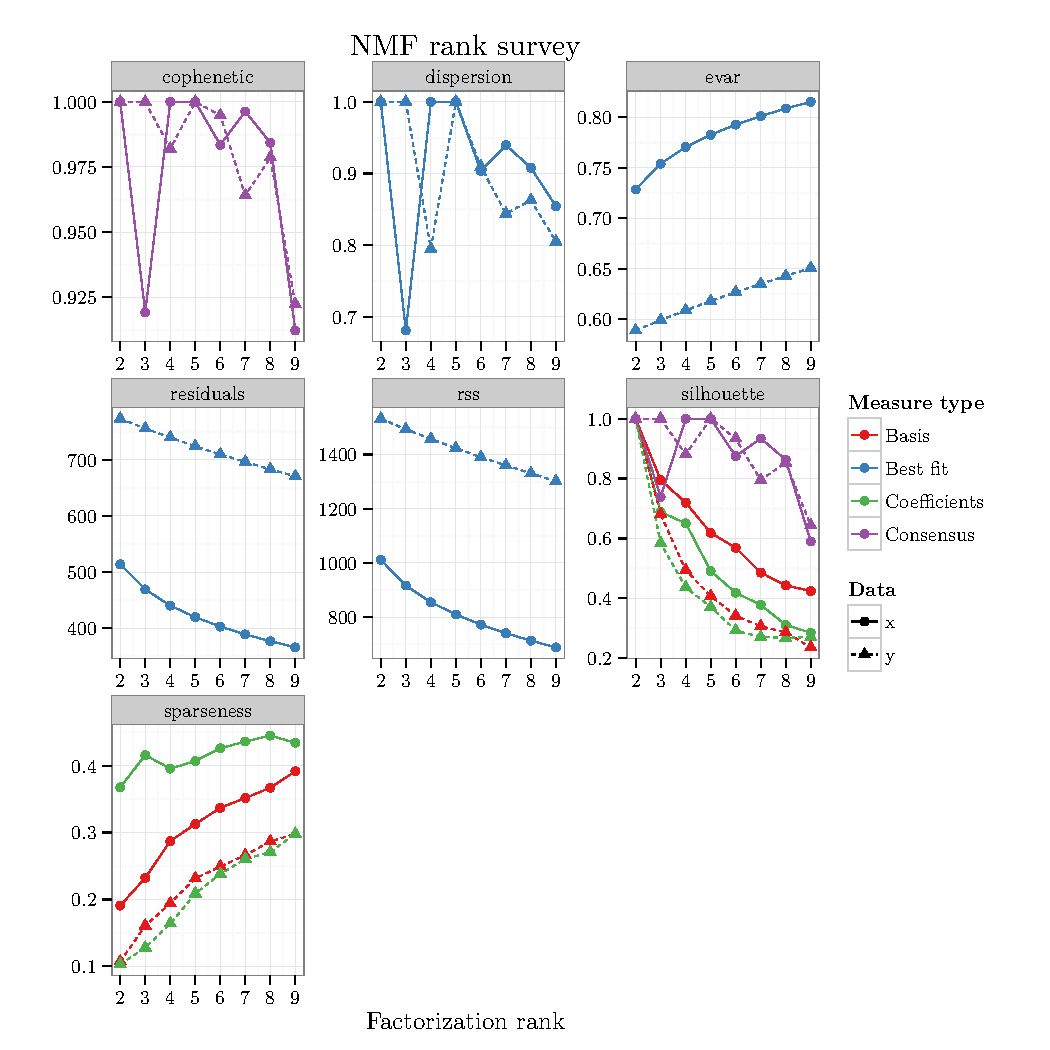
\includegraphics[width=\maxwidth]{figure/nmf-rank-plots-1} 

}


\begin{kframe}\begin{alltt}
\hlkwd{plot}\hlstd{(nmf.rankrange[}\hlopt{-}\hlnum{1}\hlstd{],} \hlopt{-}\hlstd{temp.orig_resids.delta,} \hlkwc{type} \hlstd{=} \hlstr{"o"}\hlstd{,} \hlkwc{col} \hlstd{=} \hlstr{"black"}\hlstd{,}
    \hlkwc{pch} \hlstd{=} \hlnum{21}\hlstd{,} \hlkwc{ylim} \hlstd{=} \hlkwd{range}\hlstd{(}\hlopt{-}\hlkwd{c}\hlstd{(temp.orig_resids.delta, temp.perm_resids.delta.mean)),}
    \hlkwc{xlab} \hlstd{=} \hlstr{"Factorization Rank Added"}\hlstd{,} \hlkwc{ylab} \hlstd{=} \hlstr{"Improvement in Total Residual Error"}\hlstd{)}
\hlkwd{lines}\hlstd{(nmf.rankrange[}\hlopt{-}\hlnum{1}\hlstd{],} \hlopt{-}\hlstd{temp.perm_resids.delta.mean,} \hlkwc{col} \hlstd{=} \hlstr{"red"}\hlstd{,} \hlkwc{type} \hlstd{=} \hlstr{"o"}\hlstd{,}
    \hlkwc{pch} \hlstd{=} \hlnum{21}\hlstd{,} \hlkwc{lwd} \hlstd{=} \hlnum{1}\hlstd{)}
\hlkwa{for} \hlstd{(i} \hlkwa{in} \hlnum{1}\hlopt{:}\hlkwd{ncol}\hlstd{(temp.perm_resids)) \{}
    \hlkwd{lines}\hlstd{(nmf.rankrange[}\hlopt{-}\hlnum{1}\hlstd{],} \hlopt{-}\hlstd{temp.perm_resids.delta[, i],} \hlkwc{type} \hlstd{=} \hlstr{"o"}\hlstd{,} \hlkwc{col} \hlstd{=} \hlkwd{rgb}\hlstd{(}\hlnum{1}\hlstd{,}
        \hlnum{0}\hlstd{,} \hlnum{0}\hlstd{,} \hlnum{0.25}\hlstd{))}
\hlstd{\}}
\hlkwd{lines}\hlstd{(nmf.rankrange[}\hlopt{-}\hlnum{1}\hlstd{],} \hlopt{-}\hlstd{temp.perm_resids.delta.threshold,} \hlkwc{col} \hlstd{=} \hlstr{"red"}\hlstd{,} \hlkwc{lty} \hlstd{=} \hlstr{"dotted"}\hlstd{)}
\hlkwa{if} \hlstd{(nmf.rank.wasauto} \hlopt{==} \hlnum{TRUE}\hlstd{) \{}
    \hlstd{temp.col} \hlkwb{=} \hlstr{"green"}
\hlstd{\}} \hlkwa{else} \hlstd{\{}
    \hlstd{temp.col} \hlkwb{=} \hlstr{"blue"}
\hlstd{\}}
\hlkwd{abline}\hlstd{(}\hlkwc{v} \hlstd{= nmf.rank,} \hlkwc{col} \hlstd{= temp.col,} \hlkwc{lwd} \hlstd{=} \hlnum{2}\hlstd{)}
\hlkwd{legend}\hlstd{(}\hlstr{"topright"}\hlstd{,} \hlkwc{legend} \hlstd{=} \hlkwd{c}\hlstd{(}\hlstr{"Original data"}\hlstd{,} \hlstr{"Permuted data"}\hlstd{,} \hlkwd{sprintf}\hlstd{(}\hlstr{"Selected rank (%s)"}\hlstd{,}
    \hlkwd{ifelse}\hlstd{(nmf.rank.wasauto} \hlopt{==} \hlnum{TRUE}\hlstd{,} \hlstr{"auto"}\hlstd{,} \hlstr{"fixed"}\hlstd{))),} \hlkwc{col} \hlstd{=} \hlkwd{c}\hlstd{(}\hlstr{"black"}\hlstd{,} \hlstr{"red"}\hlstd{,}
    \hlstd{temp.col),} \hlkwc{lty} \hlstd{=} \hlstr{"solid"}\hlstd{,} \hlkwc{pch} \hlstd{=} \hlnum{21}\hlstd{,} \hlkwc{inset} \hlstd{=} \hlnum{0.05}\hlstd{)}
\end{alltt}
\end{kframe}

{\centering 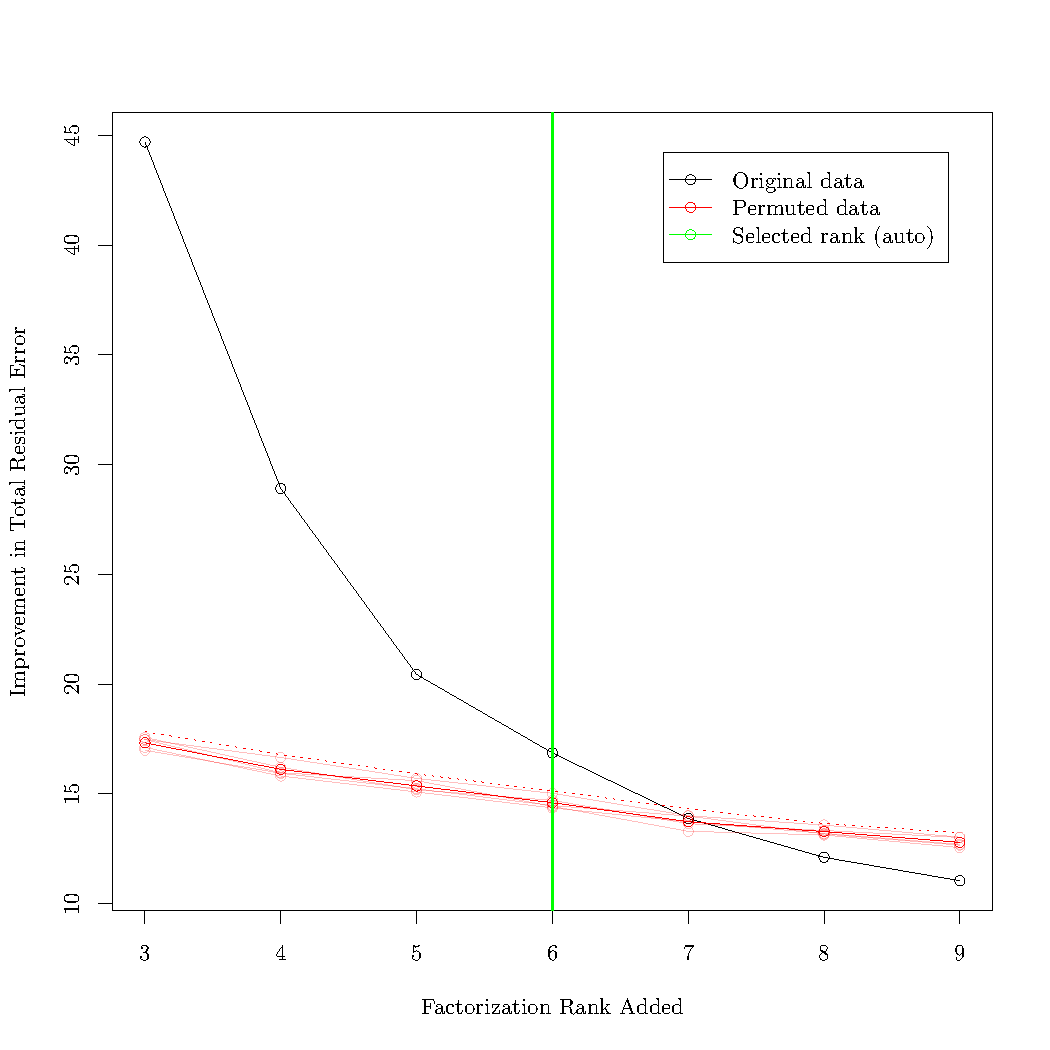
\includegraphics[width=\maxwidth]{figure/nmf-rank-plots-2} 

}



\end{knitrout}

\subsection{Fit}
\begin{knitrout}
\definecolor{shadecolor}{rgb}{0.969, 0.969, 0.969}\color{fgcolor}\begin{kframe}
\begin{alltt}
\hlkwd{consensusmap}\hlstd{(nmf.final)}
\end{alltt}
\end{kframe}

{\centering 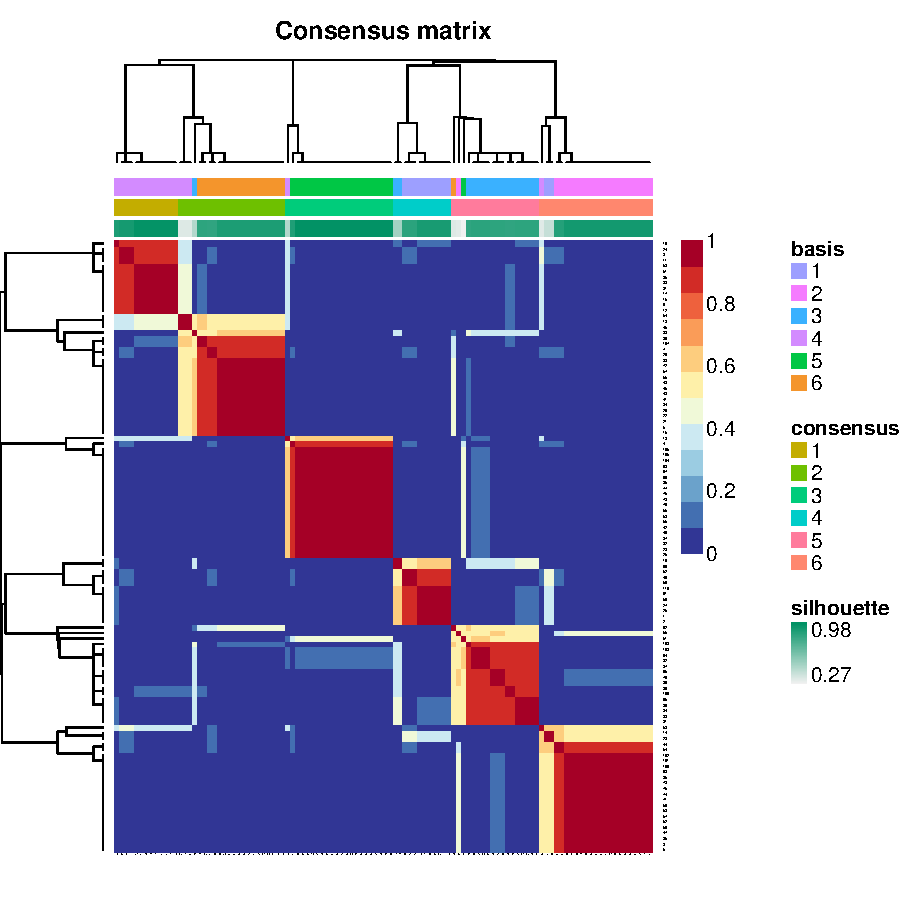
\includegraphics[width=\maxwidth]{figure/nmf-plots-1} 

}


\begin{kframe}\begin{alltt}
\hlkwd{basismap}\hlstd{(nmf.final)}
\end{alltt}
\end{kframe}

{\centering 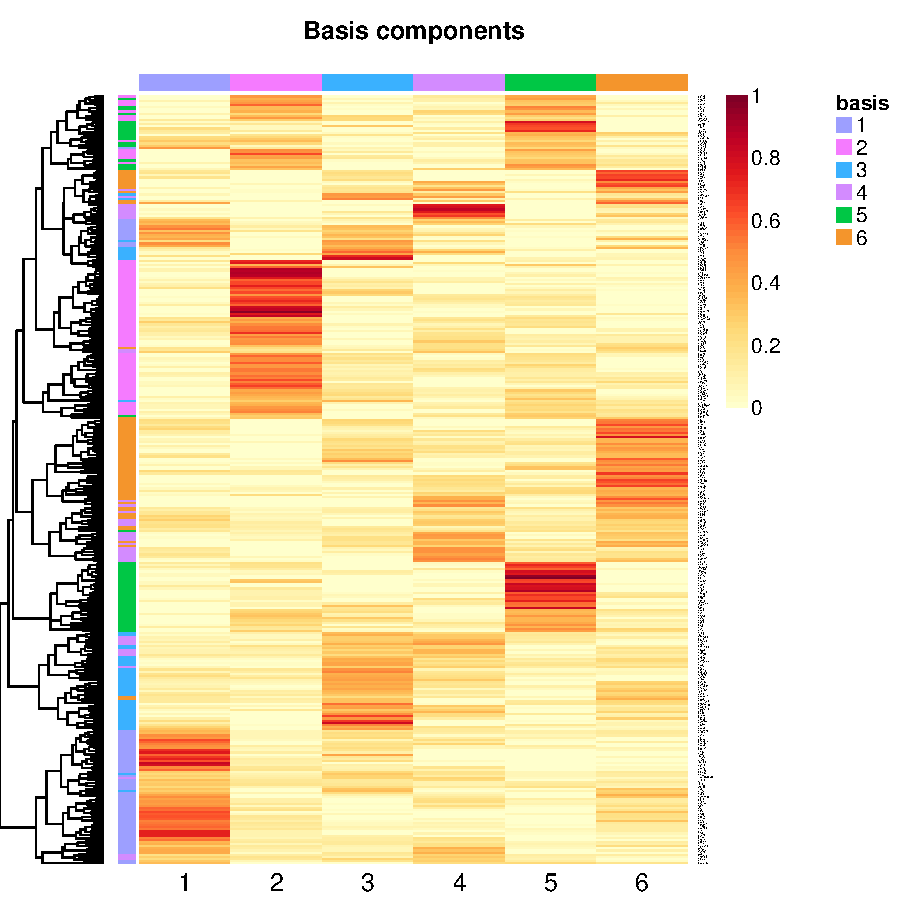
\includegraphics[width=\maxwidth]{figure/nmf-plots-2} 

}


\begin{kframe}\begin{alltt}
\hlkwd{coefmap}\hlstd{(nmf.final)}
\end{alltt}
\end{kframe}

{\centering 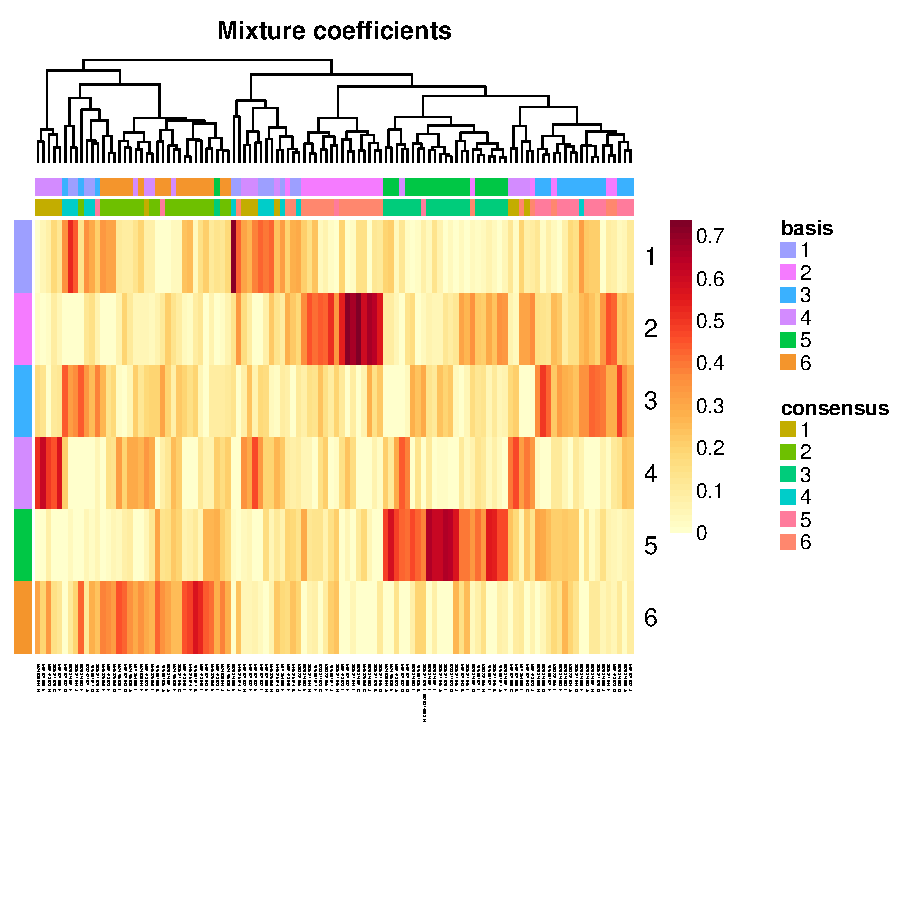
\includegraphics[width=\maxwidth]{figure/nmf-plots-3} 

}



\end{knitrout}


%%%%%%%%%%%%%%%%%%%%%%%%%%%%%%%%%%%%%%%%%%%%%%%%%%%%%%%%%%%%%%%%%%%%%%
% SIGNATURE ESTIMATION
%%%%%%%%%%%%%%%%%%%%%%%%%%%%%%%%%%%%%%%%%%%%%%%%%%%%%%%%%%%%%%%%%%%%%%
\begin{knitrout}
\definecolor{shadecolor}{rgb}{0.969, 0.969, 0.969}\color{fgcolor}\begin{kframe}
\begin{alltt}
\hlstd{coefs.diag_dsd} \hlkwb{=} \hlkwd{apply}\hlstd{(xlin.diag_dsd.sel,} \hlnum{2}\hlstd{,} \hlkwa{function}\hlstd{(}\hlkwc{xcol}\hlstd{)} \hlkwd{nnls}\hlstd{(}\hlkwd{basis}\hlstd{(nmf.final),}
    \hlstd{xcol)}\hlopt{$}\hlstd{x)}
\hlstd{coefs.diag_rec} \hlkwb{=} \hlkwd{apply}\hlstd{(xlin.diag_rec.sel,} \hlnum{2}\hlstd{,} \hlkwa{function}\hlstd{(}\hlkwc{xcol}\hlstd{)} \hlkwd{nnls}\hlstd{(}\hlkwd{basis}\hlstd{(nmf.final),}
    \hlstd{xcol)}\hlopt{$}\hlstd{x)}
\hlstd{coefs.recr_dsd} \hlkwb{=} \hlkwd{apply}\hlstd{(xlin.recr_dsd.sel,} \hlnum{2}\hlstd{,} \hlkwa{function}\hlstd{(}\hlkwc{xcol}\hlstd{)} \hlkwd{nnls}\hlstd{(}\hlkwd{basis}\hlstd{(nmf.final),}
    \hlstd{xcol)}\hlopt{$}\hlstd{x)}
\hlstd{coefs.pdac_au} \hlkwb{=} \hlkwd{apply}\hlstd{(xlin.pdac_au.sel,} \hlnum{2}\hlstd{,} \hlkwa{function}\hlstd{(}\hlkwc{xcol}\hlstd{)} \hlkwd{nnls}\hlstd{(}\hlkwd{basis}\hlstd{(nmf.final),}
    \hlstd{xcol)}\hlopt{$}\hlstd{x)}
\end{alltt}
\end{kframe}
\end{knitrout}





\begin{knitrout}
\definecolor{shadecolor}{rgb}{0.969, 0.969, 0.969}\color{fgcolor}\begin{kframe}
\begin{alltt}
\hlstd{temp.pred.pairs} \hlkwb{=} \hlkwd{t}\hlstd{(}\hlkwd{rbind}\hlstd{(coefs.pdac_au, metapcna.scores[}\hlkwd{colnames}\hlstd{(coefs.pdac_au)]))}
\hlkwd{colnames}\hlstd{(temp.pred.pairs)} \hlkwb{=} \hlkwd{paste}\hlstd{(}\hlstr{"mg"}\hlstd{,} \hlnum{1}\hlopt{:}\hlkwd{ncol}\hlstd{(temp.pred.pairs),} \hlkwc{sep} \hlstd{=} \hlstr{"."}\hlstd{)}
\hlkwd{colnames}\hlstd{(temp.pred.pairs)[}\hlkwd{ncol}\hlstd{(temp.pred.pairs)]} \hlkwb{=} \hlstr{"PCNA"}
\hlstd{temp.pred.pairs} \hlkwb{=} \hlkwd{cbind}\hlstd{(temp.pred.pairs,} \hlkwc{qpure} \hlstd{= samps.pdac_au}\hlopt{$}\hlstd{purity_qpure,}
    \hlkwc{pkyrs} \hlstd{= cpvs.pdac_au}\hlopt{$}\hlstd{History.Smoking.PackYears)}
\hlkwd{pairs}\hlstd{(temp.pred.pairs,} \hlkwc{pch} \hlstd{=} \hlnum{16}\hlstd{,} \hlkwc{cex} \hlstd{=} \hlnum{1}\hlstd{,} \hlkwc{col} \hlstd{=} \hlkwd{ifelse}\hlstd{(}\hlkwd{rownames}\hlstd{(temp.pred.pairs)} \hlopt
    \hlkwd{colnames}\hlstd{(xlin.diag_dsd.sel),} \hlkwd{rgb}\hlstd{(}\hlnum{0}\hlstd{,} \hlnum{0}\hlstd{,} \hlnum{0}\hlstd{,} \hlnum{0.5}\hlstd{),} \hlkwd{rgb}\hlstd{(}\hlnum{1}\hlstd{,} \hlnum{0}\hlstd{,} \hlnum{1}\hlstd{,} \hlnum{0.5}\hlstd{)))}
\end{alltt}
\end{kframe}

{\centering 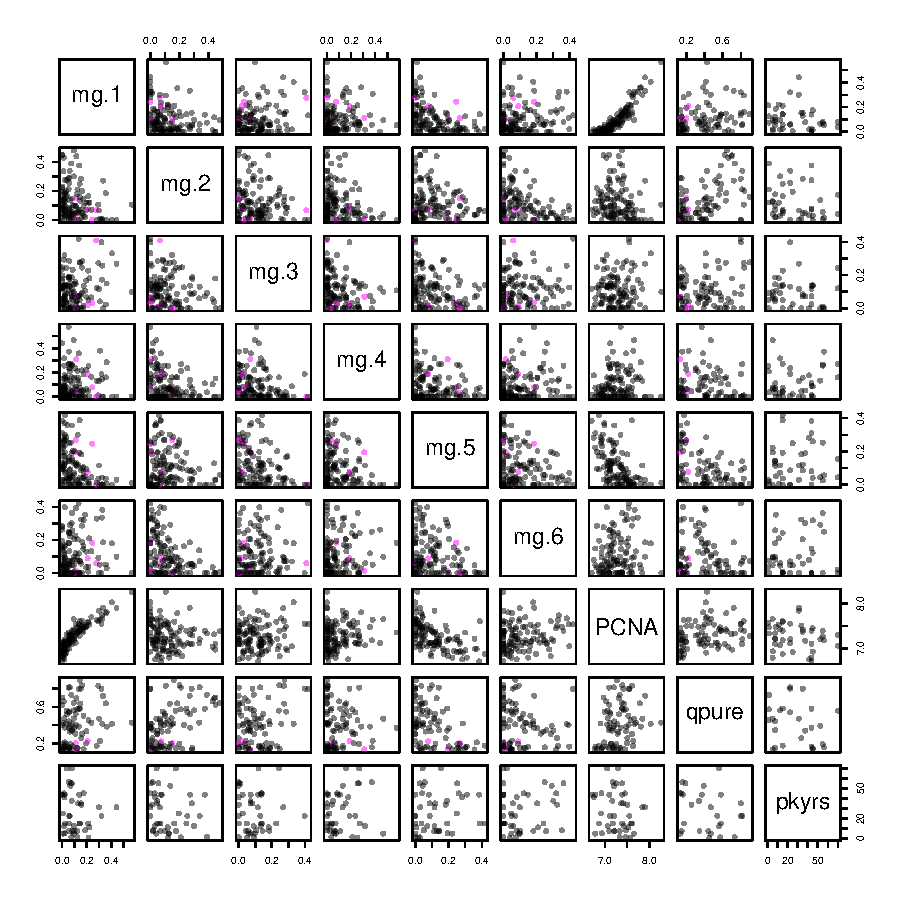
\includegraphics[width=\maxwidth]{figure/metagene-pairs-1} 

}


\begin{kframe}\begin{alltt}
\hlstd{temp.pred.pairs.rescaled} \hlkwb{=} \hlkwd{t}\hlstd{((}\hlkwd{t}\hlstd{(temp.pred.pairs)} \hlopt{-} \hlkwd{apply}\hlstd{(temp.pred.pairs,} \hlnum{2}\hlstd{,}
    \hlstd{min,} \hlkwc{na.rm} \hlstd{=} \hlnum{TRUE}\hlstd{))}\hlopt{/}\hlstd{(}\hlkwd{apply}\hlstd{(temp.pred.pairs,} \hlnum{2}\hlstd{,} \hlkwa{function}\hlstd{(}\hlkwc{x}\hlstd{)} \hlkwd{diff}\hlstd{(}\hlkwd{range}\hlstd{(x,}
    \hlkwc{na.rm} \hlstd{=} \hlnum{TRUE}\hlstd{)))))}
\hlkwd{heatmap.2}\hlstd{(temp.pred.pairs.rescaled,} \hlkwc{trace} \hlstd{=} \hlstr{"none"}\hlstd{,} \hlkwc{scale} \hlstd{=} \hlstr{"none"}\hlstd{,} \hlkwc{col} \hlstd{=} \hlkwd{brewer.pal}\hlstd{(}\hlnum{9}\hlstd{,}
    \hlstr{"GnBu"}\hlstd{))}
\end{alltt}
\end{kframe}

{\centering 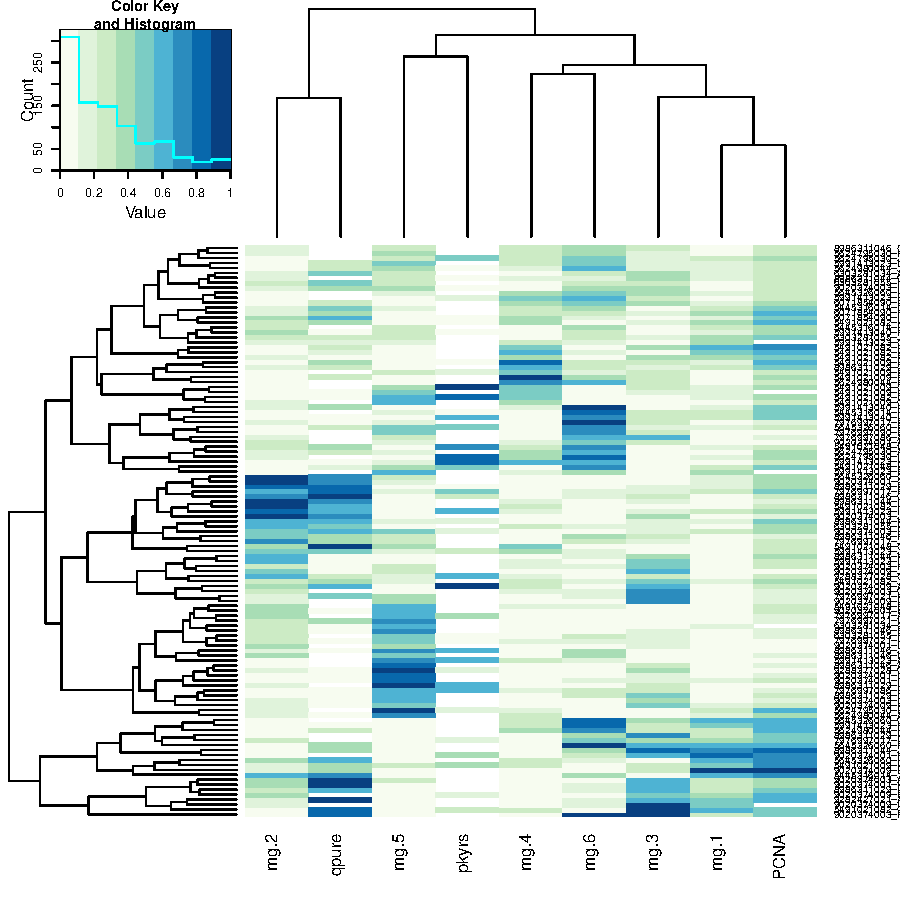
\includegraphics[width=\maxwidth]{figure/metagene-pairs-2} 

}


\begin{kframe}\begin{alltt}
\hlkwd{heatmap.2}\hlstd{(temp.pred.pairs.rescaled[}\hlkwd{apply}\hlstd{(}\hlopt{!}\hlkwd{is.na}\hlstd{(temp.pred.pairs.rescaled),} \hlnum{1}\hlstd{,}
    \hlstd{all), ],} \hlkwc{trace} \hlstd{=} \hlstr{"none"}\hlstd{,} \hlkwc{scale} \hlstd{=} \hlstr{"none"}\hlstd{,} \hlkwc{col} \hlstd{=} \hlkwd{brewer.pal}\hlstd{(}\hlnum{9}\hlstd{,} \hlstr{"GnBu"}\hlstd{))}
\end{alltt}
\end{kframe}

{\centering 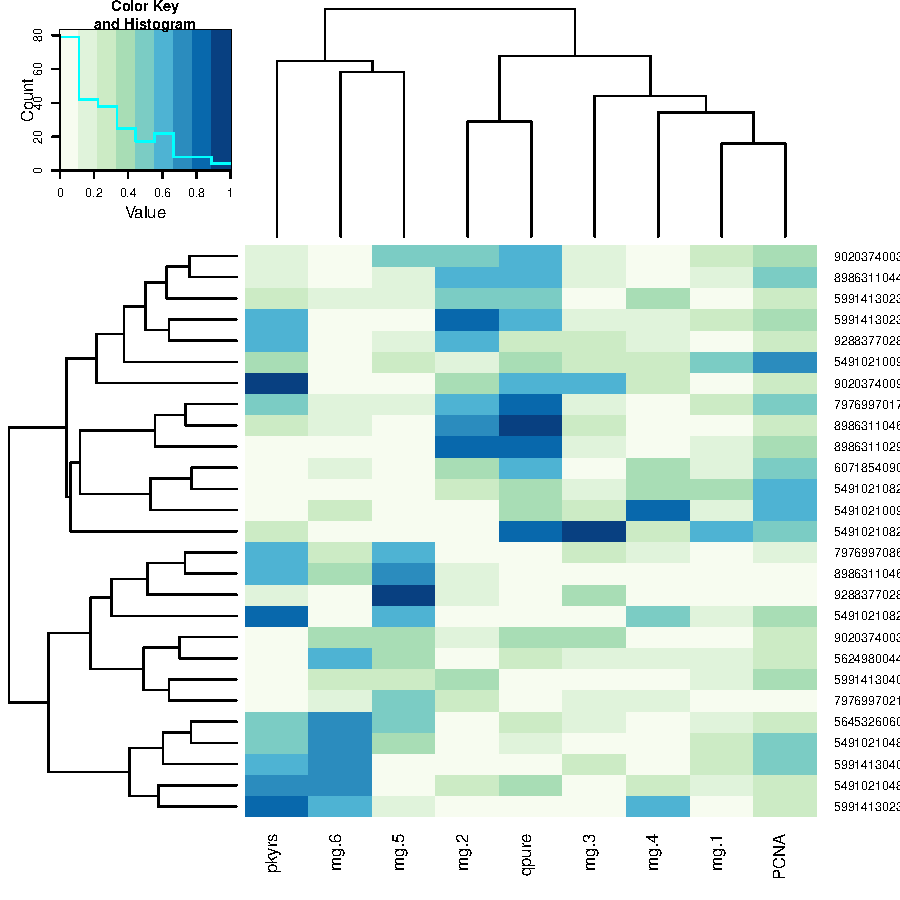
\includegraphics[width=\maxwidth]{figure/metagene-pairs-3} 

}


\begin{kframe}\begin{alltt}
\hlstd{temp.pred.pairs.rescaled2} \hlkwb{=} \hlstd{temp.pred.pairs.rescaled[,} \hlkwd{colnames}\hlstd{(temp.pred.pairs.rescaled)} \hlopt{!=}
    \hlstr{"pkyrs"}\hlstd{]}
\hlkwd{heatmap.2}\hlstd{(temp.pred.pairs.rescaled2,} \hlkwc{trace} \hlstd{=} \hlstr{"none"}\hlstd{,} \hlkwc{scale} \hlstd{=} \hlstr{"none"}\hlstd{,} \hlkwc{col} \hlstd{=} \hlkwd{brewer.pal}\hlstd{(}\hlnum{9}\hlstd{,}
    \hlstr{"GnBu"}\hlstd{))}
\end{alltt}
\end{kframe}

{\centering 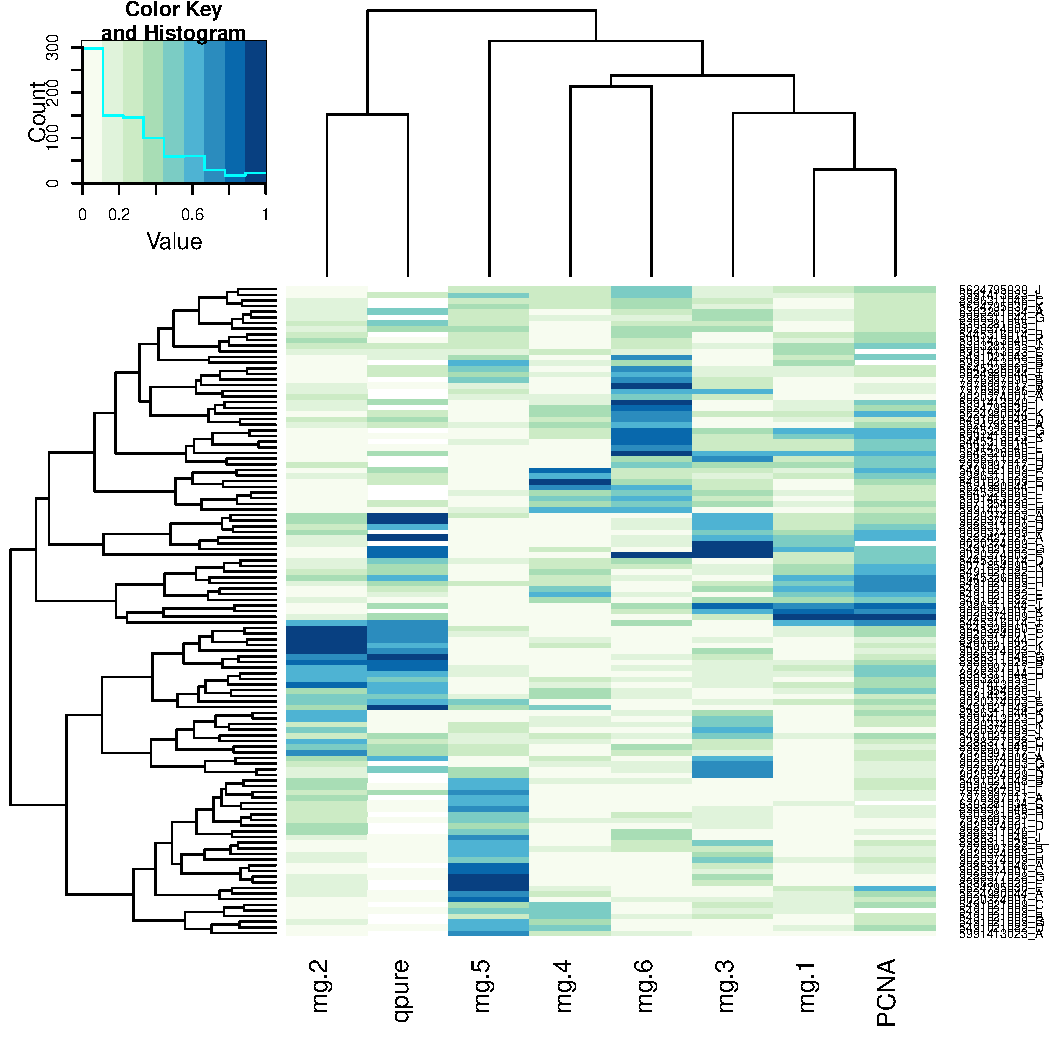
\includegraphics[width=\maxwidth]{figure/metagene-pairs-4} 

}


\begin{kframe}\begin{alltt}
\hlkwd{heatmap.2}\hlstd{(temp.pred.pairs.rescaled2[}\hlkwd{apply}\hlstd{(}\hlopt{!}\hlkwd{is.na}\hlstd{(temp.pred.pairs.rescaled2),}
    \hlnum{1}\hlstd{, all), ],} \hlkwc{trace} \hlstd{=} \hlstr{"none"}\hlstd{,} \hlkwc{scale} \hlstd{=} \hlstr{"none"}\hlstd{,} \hlkwc{col} \hlstd{=} \hlkwd{brewer.pal}\hlstd{(}\hlnum{9}\hlstd{,} \hlstr{"GnBu"}\hlstd{))}
\end{alltt}
\end{kframe}

{\centering 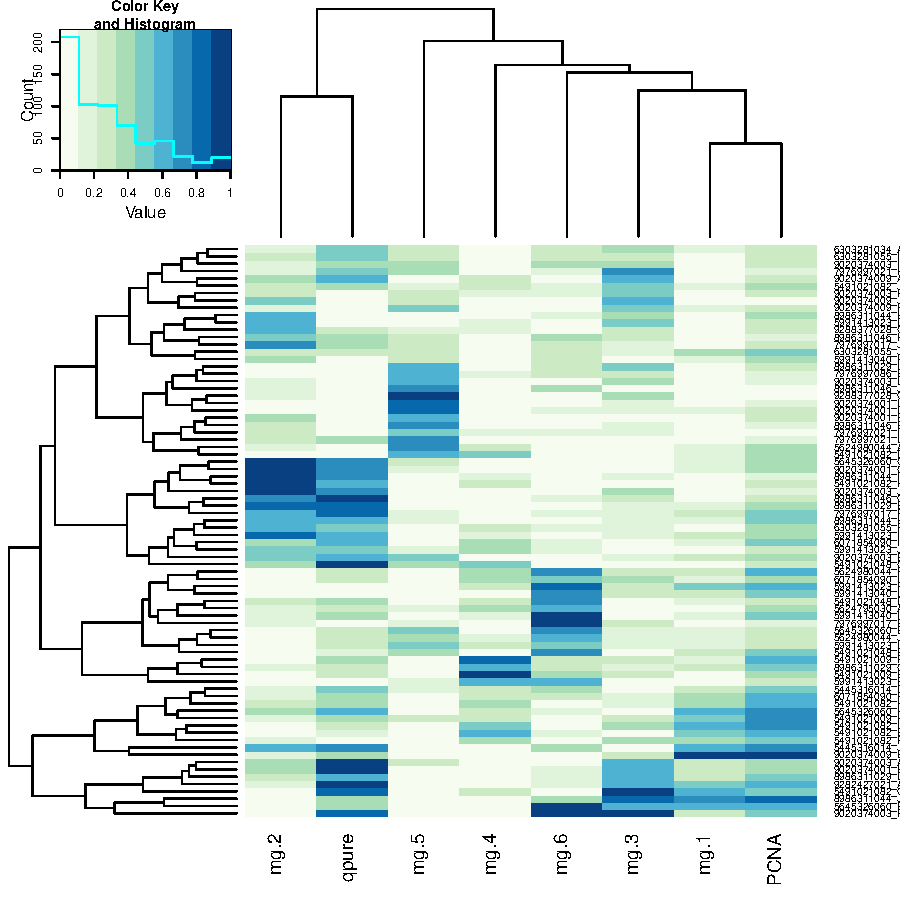
\includegraphics[width=\maxwidth]{figure/metagene-pairs-5} 

}


\begin{kframe}\begin{alltt}
\hlstd{temp.cors} \hlkwb{=} \hlkwd{apply}\hlstd{(temp.pred.pairs[,} \hlkwd{colnames}\hlstd{(temp.pred.pairs)} \hlopt{!=} \hlstr{"pkyrs"}\hlstd{],} \hlnum{2}\hlstd{,}
    \hlkwa{function}\hlstd{(}\hlkwc{x}\hlstd{)} \hlkwd{apply}\hlstd{(temp.pred.pairs[,} \hlkwd{colnames}\hlstd{(temp.pred.pairs)} \hlopt{!=} \hlstr{"pkyrs"}\hlstd{],}
        \hlnum{2}\hlstd{,} \hlkwa{function}\hlstd{(}\hlkwc{y}\hlstd{) \{}
            \hlstd{sel} \hlkwb{=} \hlopt{!}\hlstd{(}\hlkwd{is.na}\hlstd{(x)} \hlopt{|} \hlkwd{is.na}\hlstd{(y))}
            \hlkwd{cor}\hlstd{(x[sel], y[sel],} \hlkwc{method} \hlstd{=} \hlstr{"kendall"}\hlstd{)}
        \hlstd{\}))}
\hlcom{# diag(temp.cors) = NA}
\hlkwd{heatmap.2}\hlstd{(temp.cors,} \hlkwc{trace} \hlstd{=} \hlstr{"none"}\hlstd{,} \hlkwc{Rowv} \hlstd{=} \hlnum{FALSE}\hlstd{,} \hlkwc{Colv} \hlstd{=} \hlnum{FALSE}\hlstd{,} \hlkwc{col} \hlstd{=} \hlkwd{brewer.pal}\hlstd{(}\hlnum{11}\hlstd{,}
    \hlstr{"PiYG"}\hlstd{),} \hlkwc{dendrogram} \hlstd{=} \hlstr{"none"}\hlstd{,} \hlkwc{scale} \hlstd{=} \hlstr{"none"}\hlstd{)}
\end{alltt}
\end{kframe}

{\centering 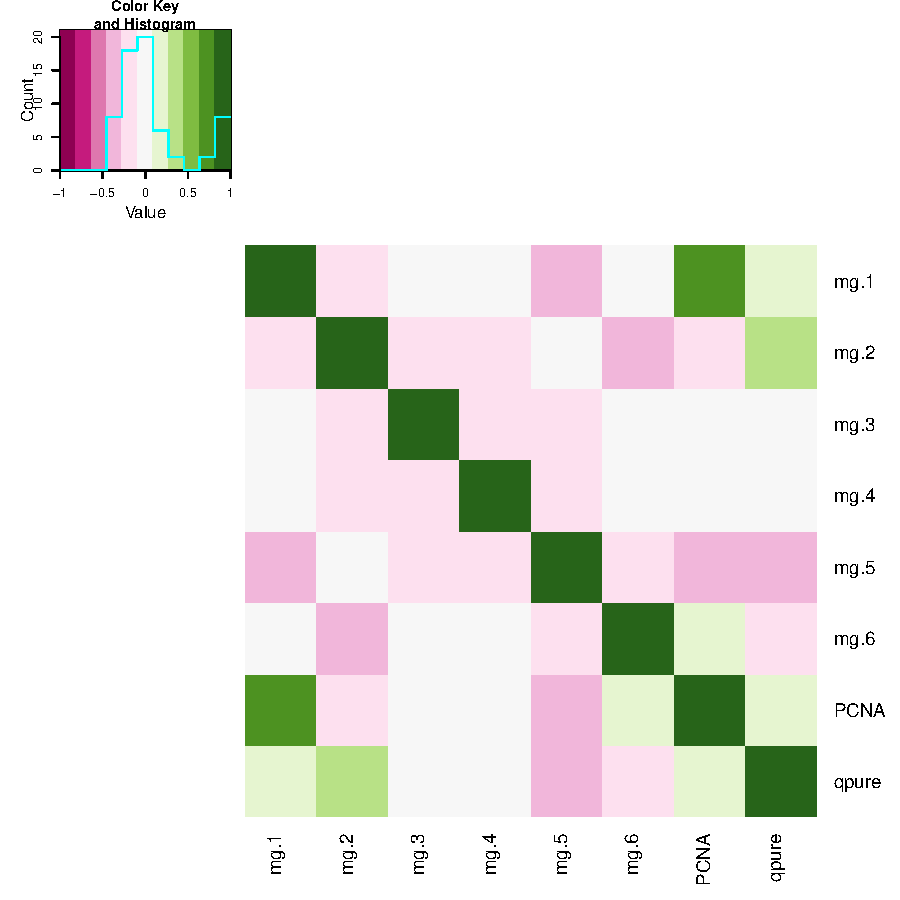
\includegraphics[width=\maxwidth]{figure/metagene-pairs-6} 

}


\begin{kframe}\begin{alltt}
\hlkwd{plot}\hlstd{(temp.pred.pairs[,} \hlstr{"mg.1"}\hlstd{]} \hlopt{~} \hlstd{temp.pred.pairs[,} \hlstr{"PCNA"}\hlstd{],} \hlkwc{col} \hlstd{=} \hlkwd{ifelse}\hlstd{(}\hlkwd{rownames}\hlstd{(temp.pred.pairs)} \hlopt
    \hlkwd{colnames}\hlstd{(xlin.diag_dsd.sel),} \hlkwd{rgb}\hlstd{(}\hlnum{0}\hlstd{,} \hlnum{0}\hlstd{,} \hlnum{0}\hlstd{,} \hlnum{1}\hlstd{),} \hlkwd{rgb}\hlstd{(}\hlnum{0}\hlstd{,} \hlnum{0}\hlstd{,} \hlnum{0}\hlstd{,} \hlnum{0}\hlstd{)),} \hlkwc{xlab} \hlstd{=} \hlstr{"Meta-PCNA Score"}\hlstd{,}
    \hlkwc{ylab} \hlstd{=} \hlstr{"MG1 Coefficient"}\hlstd{)}
\end{alltt}
\end{kframe}

{\centering 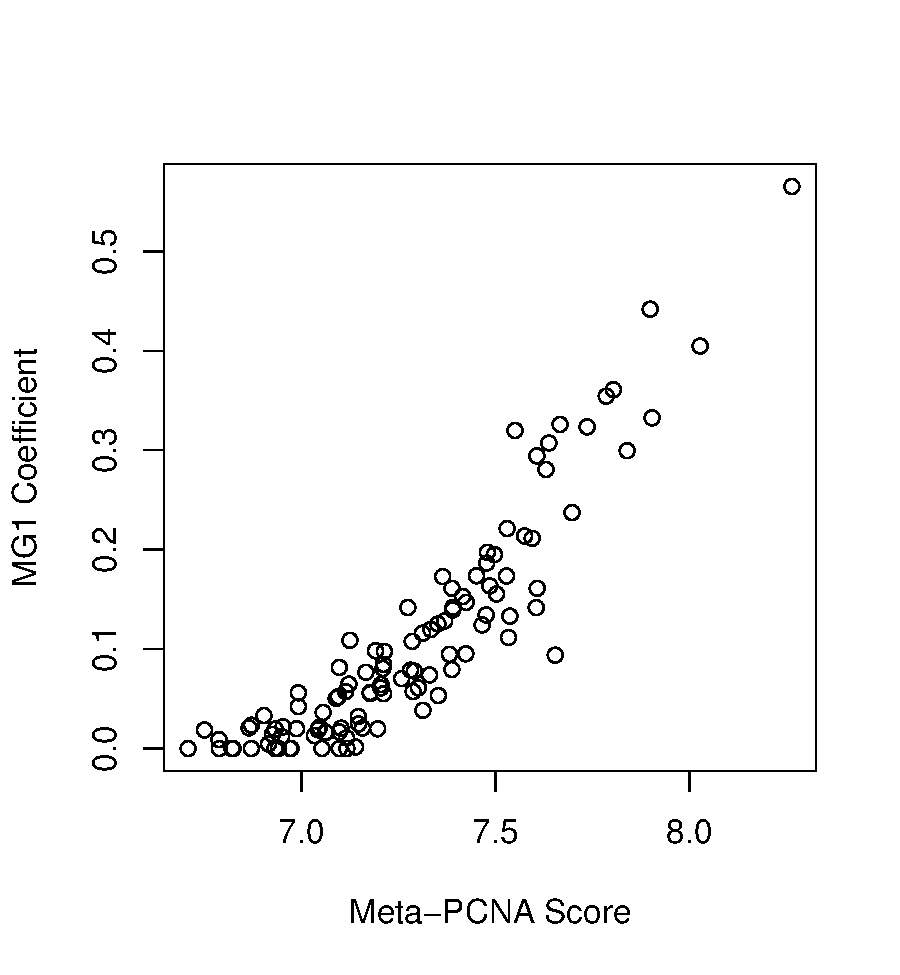
\includegraphics[width=\maxwidth]{figure/metagene-pairs-7} 

}


\begin{kframe}\begin{alltt}
\hlkwd{plot}\hlstd{(temp.pred.pairs[,} \hlstr{"mg.5"}\hlstd{], temp.pred.pairs[,} \hlstr{"mg.1"}\hlstd{],} \hlkwc{xlab} \hlstd{=} \hlstr{"MG5 Coefficient (protective)"}\hlstd{,}
    \hlkwc{ylab} \hlstd{=} \hlstr{"MG1 Coefficient (hazardous)"}\hlstd{)}
\end{alltt}
\end{kframe}

{\centering 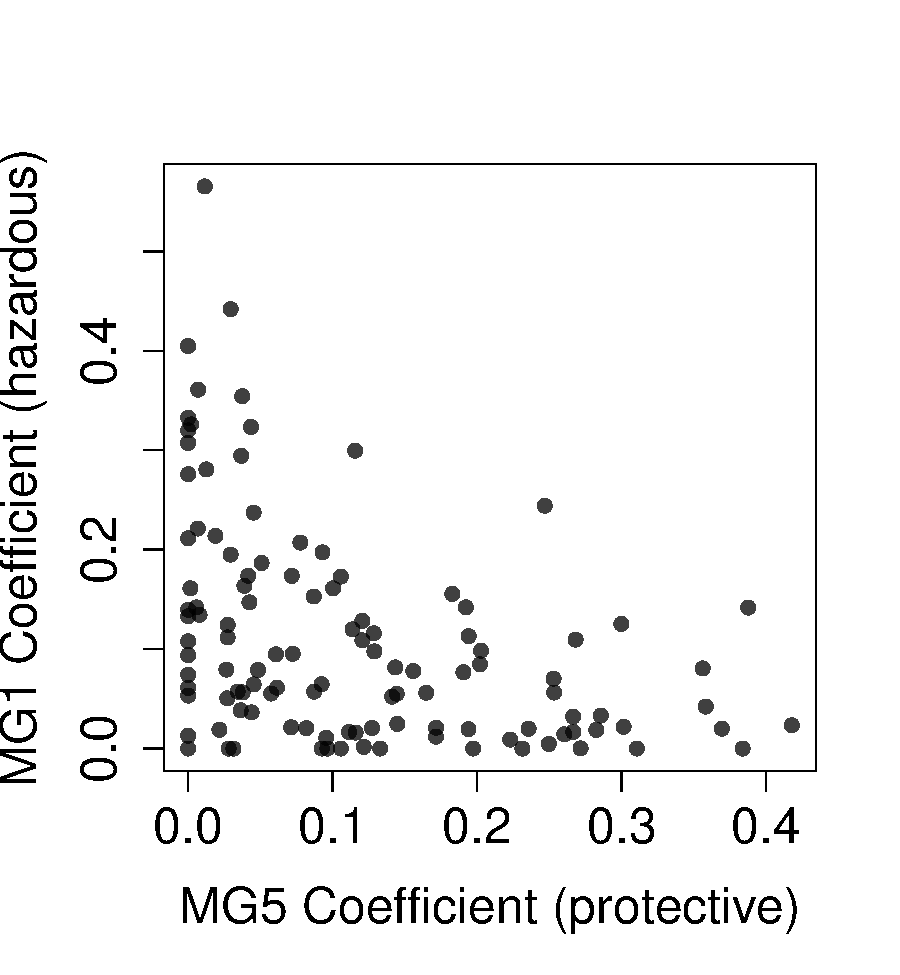
\includegraphics[width=\maxwidth]{figure/metagene-pairs-8} 

}


\begin{kframe}\begin{alltt}
\hlkwd{plot}\hlstd{(temp.pred.pairs[,} \hlstr{"mg.2"}\hlstd{], temp.pred.pairs[,} \hlstr{"mg.6"}\hlstd{],} \hlkwc{xlab} \hlstd{=} \hlstr{"MG2 Coefficient (protective)"}\hlstd{,}
    \hlkwc{ylab} \hlstd{=} \hlstr{"MG6 Coefficient"}\hlstd{)}
\end{alltt}
\end{kframe}

{\centering 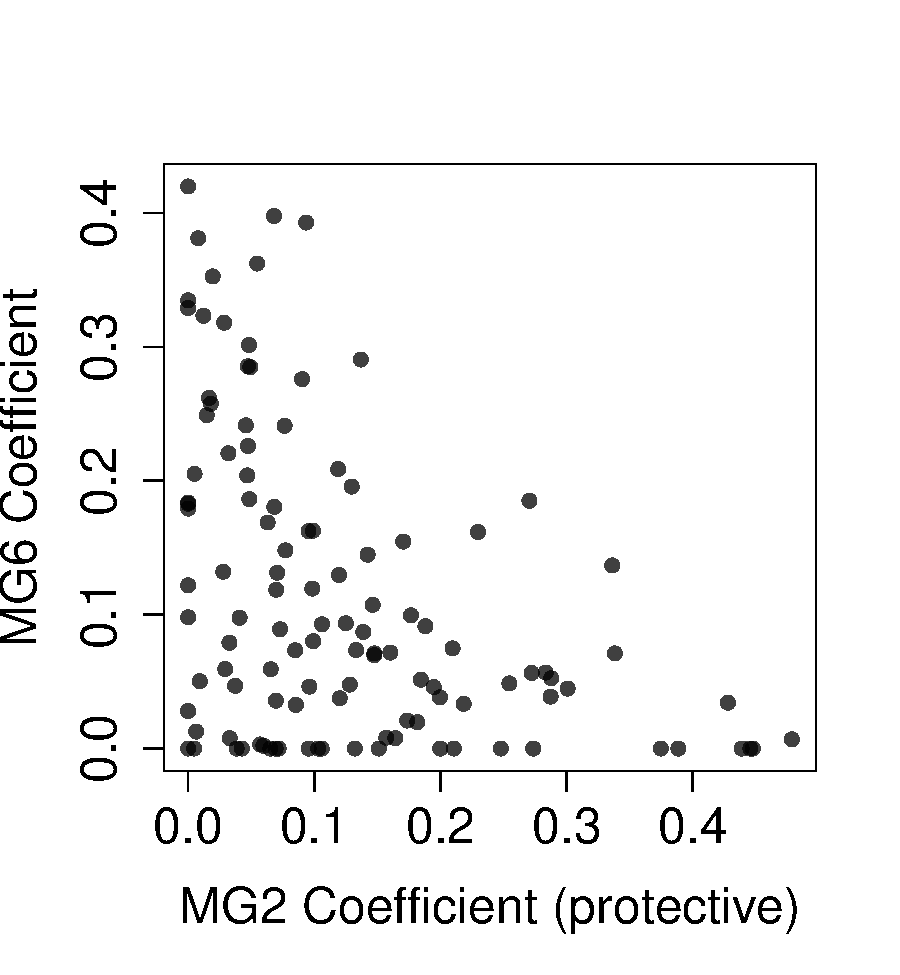
\includegraphics[width=\maxwidth]{figure/metagene-pairs-9} 

}


\begin{kframe}\begin{alltt}
\hlcom{# scatter.smooth(temp.pred.pairs[,'mg.5'], temp.pred.pairs[,'mg.1'], xlab =}
\hlcom{# 'MG5 Coefficient (protective)', ylab = 'MG1 Coefficient (hazardous)', span}
\hlcom{# = 1/4, lpars = list(lwd = 2, col = rgb(0, 0, 0, 0.5)))}
\hlcom{# scatter.smooth(temp.pred.pairs[,'mg.2'], temp.pred.pairs[,'mg.6'], xlab =}
\hlcom{# 'MG2 Coefficient (protective)', ylab = 'MG6 Coefficient', span = 1/4,}
\hlcom{# lpars = list(lwd = 2, col = rgb(0, 0, 1, 0.5)))}
\hlcom{# smoothScatter(temp.pred.pairs[,'mg.5'], temp.pred.pairs[,'mg.1'], xlab =}
\hlcom{# 'MG5 Coefficient (protective)', ylab = 'MG1 Coefficient (hazardous)')}
\hlcom{# smoothScatter(temp.pred.pairs[,'mg.2'], temp.pred.pairs[,'mg.6'], xlab =}
\hlcom{# 'MG2 Coefficient (protective)', ylab = 'MG6 Coefficient')}

\hlstd{temp.coefs.pdcor} \hlkwb{=} \hlkwd{apply}\hlstd{(coefs.diag_dsd,} \hlnum{1}\hlstd{,} \hlkwa{function}\hlstd{(}\hlkwc{x1}\hlstd{)} \hlkwd{apply}\hlstd{(coefs.diag_dsd,}
    \hlnum{1}\hlstd{,} \hlkwa{function}\hlstd{(}\hlkwc{x2}\hlstd{)} \hlkwd{dcov.test}\hlstd{(x1, x2,} \hlkwc{R} \hlstd{=} \hlnum{9999}\hlstd{)}\hlopt{$}\hlstd{p.value))}
\hlstd{temp.coefs.pfisher} \hlkwb{=} \hlkwd{apply}\hlstd{(coefs.diag_dsd,} \hlnum{1}\hlstd{,} \hlkwa{function}\hlstd{(}\hlkwc{x1}\hlstd{)} \hlkwd{apply}\hlstd{(coefs.diag_dsd,}
    \hlnum{1}\hlstd{,} \hlkwa{function}\hlstd{(}\hlkwc{x2}\hlstd{)} \hlkwd{fisher.test}\hlstd{(x1} \hlopt{>} \hlkwd{median}\hlstd{(x1), x2} \hlopt{>} \hlkwd{median}\hlstd{(x2))}\hlopt{$}\hlstd{p.value))}
\hlkwd{diag}\hlstd{(temp.coefs.pdcor)} \hlkwb{=} \hlnum{NA}
\hlstd{temp.coefs.pdcor[}\hlkwd{lower.tri}\hlstd{(temp.coefs.pdcor)]} \hlkwb{=} \hlnum{NA}
\hlkwd{diag}\hlstd{(temp.coefs.pfisher)} \hlkwb{=} \hlnum{NA}
\hlstd{temp.coefs.pfisher[}\hlkwd{lower.tri}\hlstd{(temp.coefs.pfisher)]} \hlkwb{=} \hlnum{NA}
\hlstd{temp.coefs.pdcor.holm} \hlkwb{=} \hlkwd{matrix}\hlstd{(}\hlkwd{p.adjust}\hlstd{(temp.coefs.pdcor,} \hlstr{"holm"}\hlstd{),} \hlkwc{nrow} \hlstd{=} \hlkwd{nrow}\hlstd{(temp.coefs.pdcor))}
\hlstd{temp.coefs.pfisher.holm} \hlkwb{=} \hlkwd{matrix}\hlstd{(}\hlkwd{p.adjust}\hlstd{(temp.coefs.pfisher,} \hlstr{"holm"}\hlstd{),} \hlkwc{nrow} \hlstd{=} \hlkwd{nrow}\hlstd{(temp.coefs.pfisher))}
\hlstd{temp.coefs.pdcor.holm}
\end{alltt}
\begin{verbatim}
##      [,1]   [,2]   [,3]   [,4]   [,5]   [,6]
## [1,]   NA 0.2016 0.4500 1.0000 0.0015 1.0000
## [2,]   NA     NA 0.3066 0.0130 0.1800 0.0015
## [3,]   NA     NA     NA 0.0336 0.0451 1.0000
## [4,]   NA     NA     NA     NA 0.0480 1.0000
## [5,]   NA     NA     NA     NA     NA 0.0480
## [6,]   NA     NA     NA     NA     NA     NA
\end{verbatim}
\begin{alltt}
\hlstd{temp.coefs.pfisher.holm}
\end{alltt}
\begin{verbatim}
##      [,1] [,2]   [,3] [,4]    [,5]    [,6]
## [1,]   NA    1 1.0000    1 0.03203 1.00000
## [2,]   NA   NA 0.7286    1 1.00000 0.03203
## [3,]   NA   NA     NA    1 1.00000 1.00000
## [4,]   NA   NA     NA   NA 0.72858 1.00000
## [5,]   NA   NA     NA   NA      NA 1.00000
## [6,]   NA   NA     NA   NA      NA      NA
\end{verbatim}
\begin{alltt}
\hlkwd{dcov.test}\hlstd{(coefs.diag_dsd[}\hlnum{5}\hlstd{, ], coefs.diag_dsd[}\hlnum{1}\hlstd{, ],} \hlkwc{R} \hlstd{=} \hlnum{19999}\hlstd{)}
\end{alltt}
\begin{verbatim}
## 
## 	dCov test of independence
## 
## data:  index 1, replicates 19999
## nV^2 = 0.1291, p-value = 5e-05
## sample estimates:
##    dCov 
## 0.03426
\end{verbatim}
\begin{alltt}
\hlkwd{dcov.test}\hlstd{(coefs.diag_dsd[}\hlnum{2}\hlstd{, ], coefs.diag_dsd[}\hlnum{6}\hlstd{, ],} \hlkwc{R} \hlstd{=} \hlnum{19999}\hlstd{)}
\end{alltt}
\begin{verbatim}
## 
## 	dCov test of independence
## 
## data:  index 1, replicates 19999
## nV^2 = 0.1396, p-value = 5e-05
## sample estimates:
##    dCov 
## 0.03562
\end{verbatim}
\begin{alltt}
\hlkwd{cor.test}\hlstd{(coefs.diag_dsd[}\hlnum{5}\hlstd{, ], coefs.diag_dsd[}\hlnum{1}\hlstd{, ],} \hlkwc{method} \hlstd{=} \hlstr{"kendall"}\hlstd{)}
\end{alltt}
\begin{verbatim}
## 
## 	Kendall's rank correlation tau
## 
## data:  coefs.diag_dsd[5, ] and coefs.diag_dsd[1, ]
## z = -4.97, p-value = 6.694e-07
## alternative hypothesis: true tau is not equal to 0
## sample estimates:
##     tau 
## -0.3243
\end{verbatim}
\begin{alltt}
\hlkwd{cor.test}\hlstd{(coefs.diag_dsd[}\hlnum{2}\hlstd{, ], coefs.diag_dsd[}\hlnum{6}\hlstd{, ],} \hlkwc{method} \hlstd{=} \hlstr{"kendall"}\hlstd{)}
\end{alltt}
\begin{verbatim}
## 
## 	Kendall's rank correlation tau
## 
## data:  coefs.diag_dsd[2, ] and coefs.diag_dsd[6, ]
## z = -4.931, p-value = 8.195e-07
## alternative hypothesis: true tau is not equal to 0
## sample estimates:
##     tau 
## -0.3236
\end{verbatim}
\begin{alltt}
\hlstd{temp.axis1} \hlkwb{=} \hlstd{coefs.diag_dsd[}\hlnum{1}\hlstd{, ]} \hlopt{-} \hlstd{coefs.diag_dsd[}\hlnum{5}\hlstd{, ]}
\hlstd{temp.axis2} \hlkwb{=} \hlstd{coefs.diag_dsd[}\hlnum{6}\hlstd{, ]} \hlopt{-} \hlstd{coefs.diag_dsd[}\hlnum{2}\hlstd{, ]}
\hlkwd{dcov.test}\hlstd{(temp.axis1, temp.axis2,} \hlkwc{R} \hlstd{=} \hlnum{19999}\hlstd{)}
\end{alltt}
\begin{verbatim}
## 
## 	dCov test of independence
## 
## data:  index 1, replicates 19999
## nV^2 = 0.1074, p-value = 0.0197
## sample estimates:
##    dCov 
## 0.03124
\end{verbatim}
\begin{alltt}
\hlkwd{cor.test}\hlstd{(temp.axis1, temp.axis2,} \hlkwc{method} \hlstd{=} \hlstr{"kendall"}\hlstd{)}
\end{alltt}
\begin{verbatim}
## 
## 	Kendall's rank correlation tau
## 
## data:  temp.axis1 and temp.axis2
## z = 1.253, p-value = 0.2103
## alternative hypothesis: true tau is not equal to 0
## sample estimates:
##    tau 
## 0.0809
\end{verbatim}
\begin{alltt}
\hlkwd{plot}\hlstd{(temp.axis2} \hlopt{~} \hlstd{temp.axis1,} \hlkwc{xlab} \hlstd{=} \hlstr{"Axis 1 activity"}\hlstd{,} \hlkwc{ylab} \hlstd{=} \hlstr{"Axis 2 activity"}\hlstd{)}
\end{alltt}
\end{kframe}

{\centering 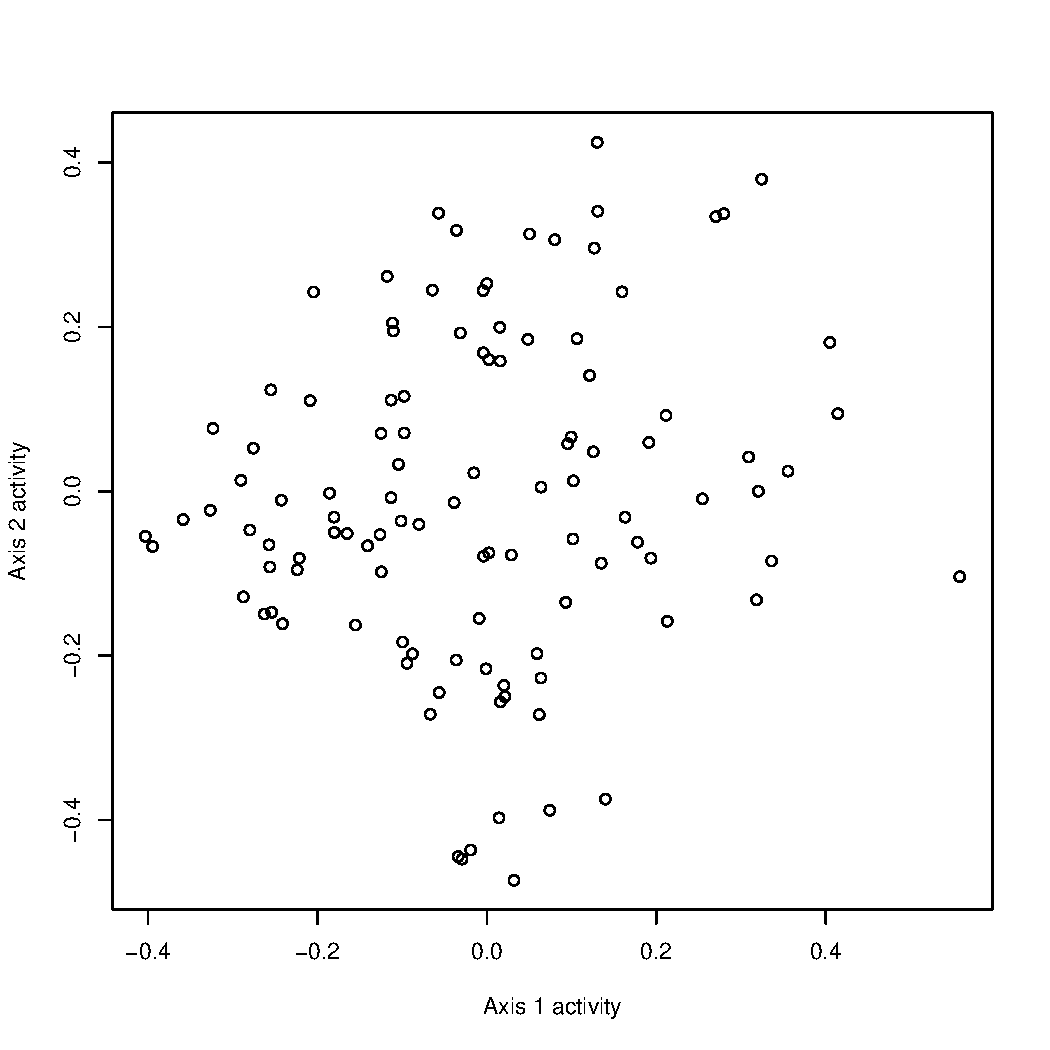
\includegraphics[width=\maxwidth]{figure/metagene-pairs-10} 

}


\begin{kframe}\begin{alltt}
\hlkwd{coxph}\hlstd{(y.diag_dsd} \hlopt{~} \hlstd{temp.axis1} \hlopt{*} \hlstd{temp.axis2)}
\end{alltt}
\begin{verbatim}
## Call:
## coxph(formula = y.diag_dsd ~ temp.axis1 * temp.axis2)
## 
## 
##                       coef exp(coef) se(coef)    z       p
## temp.axis1            3.19      24.2    0.676 4.72 2.4e-06
## temp.axis2            2.89      18.0    0.657 4.40 1.1e-05
## temp.axis1:temp.axis2 5.03     153.1    4.189 1.20 2.3e-01
## 
## Likelihood ratio test=48  on 3 df, p=2.12e-10  n= 110, number of events= 70
\end{verbatim}
\begin{alltt}
\hlstd{temp} \hlkwb{=} \hlkwd{cv.glmnet}\hlstd{(}\hlkwd{cbind}\hlstd{(temp.axis1, temp.axis2, temp.axis1} \hlopt{*} \hlstd{temp.axis2), y.diag_dsd,}
    \hlkwc{family} \hlstd{=} \hlstr{"cox"}\hlstd{,} \hlkwc{nfolds} \hlstd{=} \hlnum{10}\hlstd{)}
\hlkwd{plot}\hlstd{(temp)}
\end{alltt}
\end{kframe}

{\centering 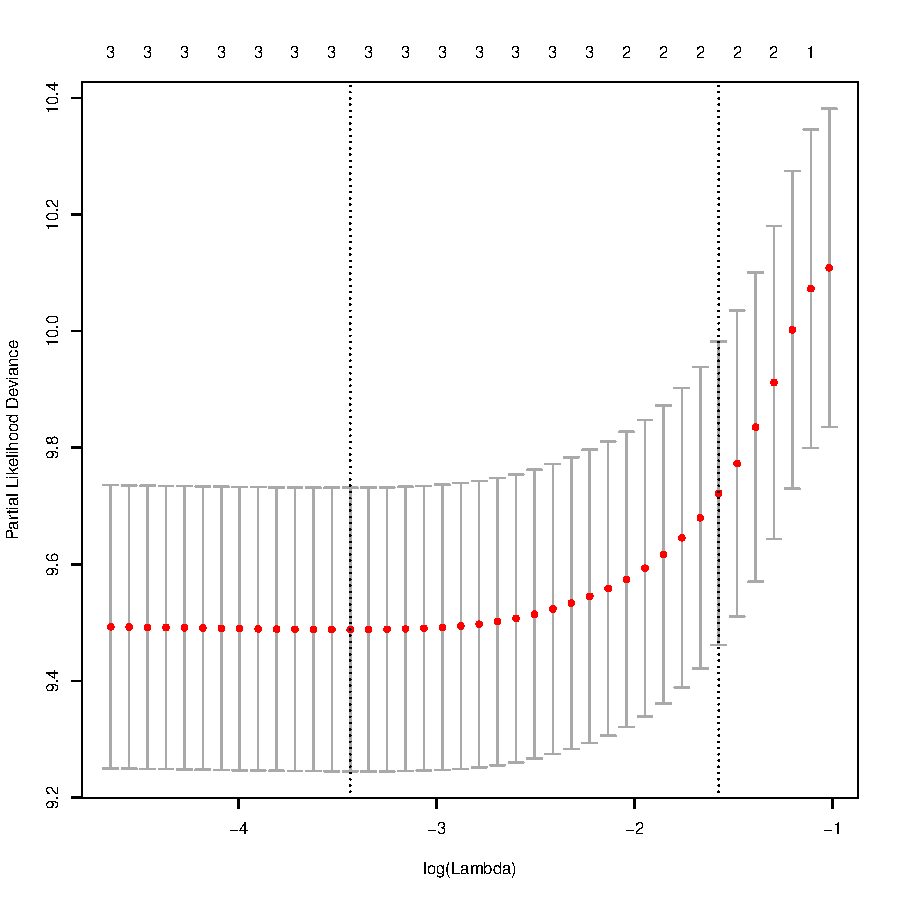
\includegraphics[width=\maxwidth]{figure/metagene-pairs-11} 

}


\begin{kframe}\begin{alltt}
\hlkwd{plot}\hlstd{(temp}\hlopt{$}\hlstd{glmnet.fit,} \hlkwc{label} \hlstd{=} \hlnum{TRUE}\hlstd{)}
\hlkwd{abline}\hlstd{(}\hlkwc{v} \hlstd{=} \hlkwd{sum}\hlstd{(}\hlkwd{abs}\hlstd{(}\hlkwd{coef}\hlstd{(temp}\hlopt{$}\hlstd{glmnet.fit,} \hlkwc{s} \hlstd{= temp}\hlopt{$}\hlstd{lambda.1se))))}
\hlkwd{abline}\hlstd{(}\hlkwc{v} \hlstd{=} \hlkwd{sum}\hlstd{(}\hlkwd{abs}\hlstd{(}\hlkwd{coef}\hlstd{(temp}\hlopt{$}\hlstd{glmnet.fit,} \hlkwc{s} \hlstd{= temp}\hlopt{$}\hlstd{lambda.min))))}
\end{alltt}
\end{kframe}

{\centering 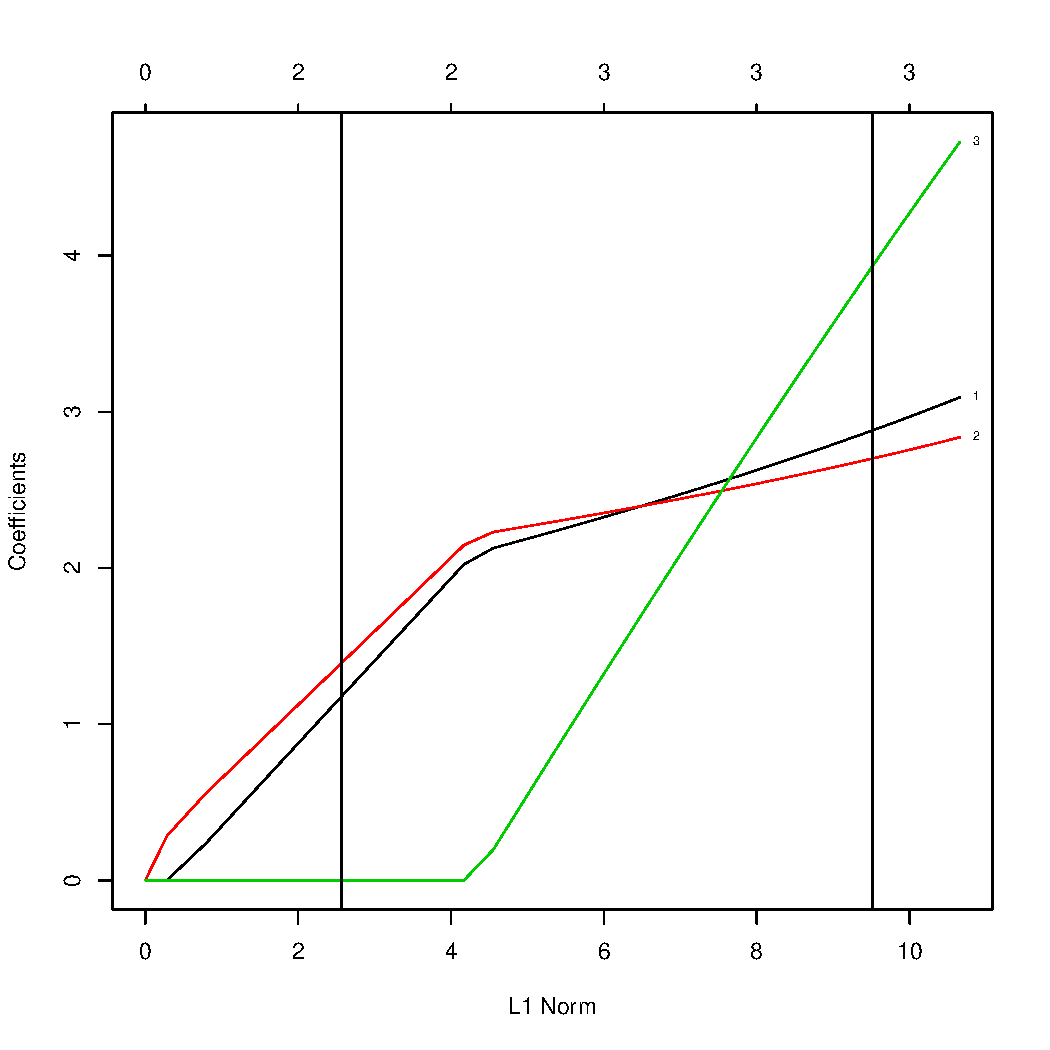
\includegraphics[width=\maxwidth]{figure/metagene-pairs-12} 

}


\begin{kframe}\begin{alltt}
\hlkwd{coef}\hlstd{(temp}\hlopt{$}\hlstd{glmnet.fit,} \hlkwc{s} \hlstd{= temp}\hlopt{$}\hlstd{lambda.1se)}
\end{alltt}
\begin{verbatim}
## 3 x 1 sparse Matrix of class "dgCMatrix"
##                1
## temp.axis1 1.176
## temp.axis2 1.390
##            .
\end{verbatim}
\end{kframe}
\end{knitrout}


%%%%%%%%%%%%%%%%%%%%%%%%%%%%%%%%%%%%%%%%%%%%%%%%%%%%%%%%%%%%%%%%%%%%%%
% SIGNATURE PROGNOSTIC PERFORMANCE: TRAINING SET, ALONE
%%%%%%%%%%%%%%%%%%%%%%%%%%%%%%%%%%%%%%%%%%%%%%%%%%%%%%%%%%%%%%%%%%%%%%
\subsection{LASSO on training set}
\begin{knitrout}
\definecolor{shadecolor}{rgb}{0.969, 0.969, 0.969}\color{fgcolor}\begin{kframe}
\begin{alltt}
\hlstd{glmnet.fit.cv.diag_dsd} \hlkwb{=} \hlkwd{cv.glmnet}\hlstd{(}\hlkwd{t}\hlstd{(coefs.diag_dsd), y.diag_dsd,} \hlkwc{family} \hlstd{=} \hlstr{"cox"}\hlstd{,}
    \hlkwc{nfolds} \hlstd{=} \hlnum{10}\hlstd{)}
\hlstd{glmnet.fit.cv.diag_rec} \hlkwb{=} \hlkwd{cv.glmnet}\hlstd{(}\hlkwd{t}\hlstd{(coefs.diag_rec), y.diag_rec,} \hlkwc{family} \hlstd{=} \hlstr{"cox"}\hlstd{,}
    \hlkwc{nfolds} \hlstd{=} \hlnum{10}\hlstd{)}
\hlstd{glmnet.fit.cv.recr_dsd} \hlkwb{=} \hlkwd{cv.glmnet}\hlstd{(}\hlkwd{t}\hlstd{(coefs.recr_dsd), y.recr_dsd,} \hlkwc{family} \hlstd{=} \hlstr{"cox"}\hlstd{,}
    \hlkwc{nfolds} \hlstd{=} \hlnum{10}\hlstd{)}
\hlstd{axis_coefs.diag_dsd} \hlkwb{=} \hlkwd{as.matrix}\hlstd{(}\hlkwd{cbind}\hlstd{(}\hlkwc{axis1} \hlstd{= coefs.diag_dsd[}\hlnum{1}\hlstd{, ]} \hlopt{-} \hlstd{coefs.diag_dsd[}\hlnum{5}\hlstd{,}
    \hlstd{],} \hlkwc{axis2} \hlstd{= coefs.diag_dsd[}\hlnum{6}\hlstd{, ]} \hlopt{-} \hlstd{coefs.diag_dsd[}\hlnum{2}\hlstd{, ]))}
\end{alltt}
\end{kframe}
\end{knitrout}

\begin{knitrout}
\definecolor{shadecolor}{rgb}{0.969, 0.969, 0.969}\color{fgcolor}\begin{kframe}
\begin{alltt}
\hlkwd{plot}\hlstd{(glmnet.fit.cv.diag_dsd)}
\end{alltt}
\end{kframe}

{\centering 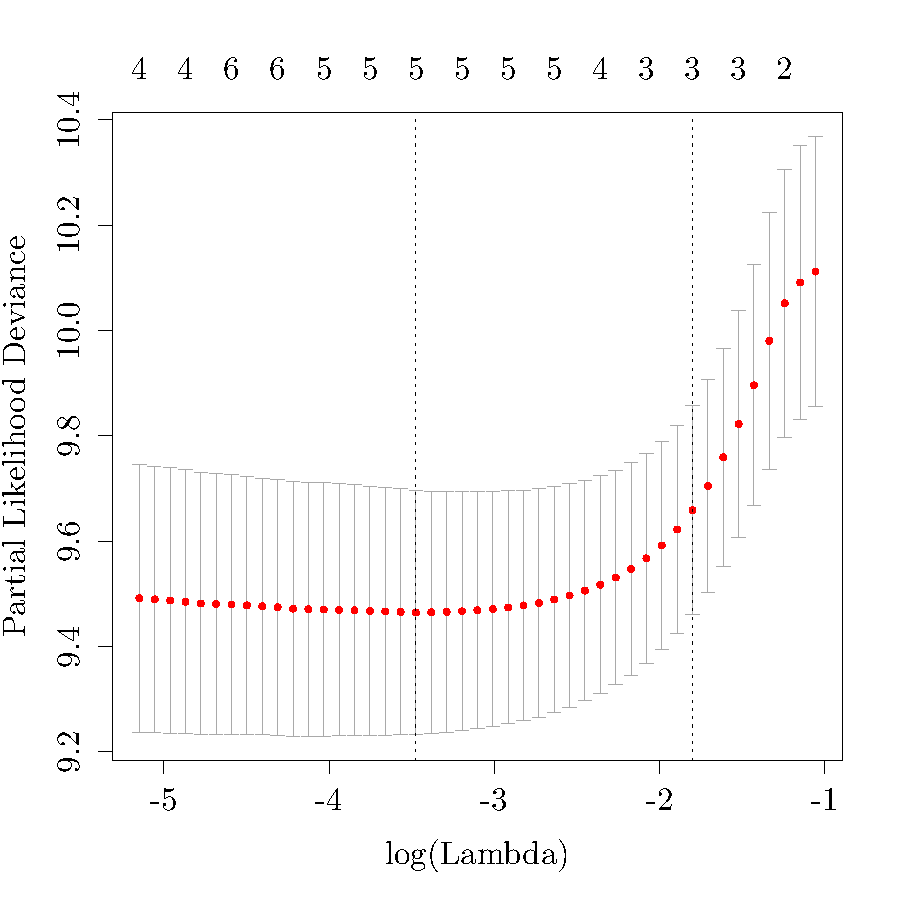
\includegraphics[width=\maxwidth]{figure/nmf-metagene-glmnet-plots-1} 

}


\begin{kframe}\begin{alltt}
\hlkwd{plot}\hlstd{(glmnet.fit.cv.diag_dsd}\hlopt{$}\hlstd{glmnet.fit,} \hlkwc{label} \hlstd{=} \hlnum{TRUE}\hlstd{)}
\hlkwd{abline}\hlstd{(}\hlkwc{v} \hlstd{=} \hlkwd{sum}\hlstd{(}\hlkwd{abs}\hlstd{(}\hlkwd{coef}\hlstd{(glmnet.fit.cv.diag_dsd}\hlopt{$}\hlstd{glmnet.fit,} \hlkwc{s} \hlstd{= glmnet.fit.cv.diag_dsd}\hlopt{$}\hlstd{lambda.1se))))}
\end{alltt}
\end{kframe}

{\centering 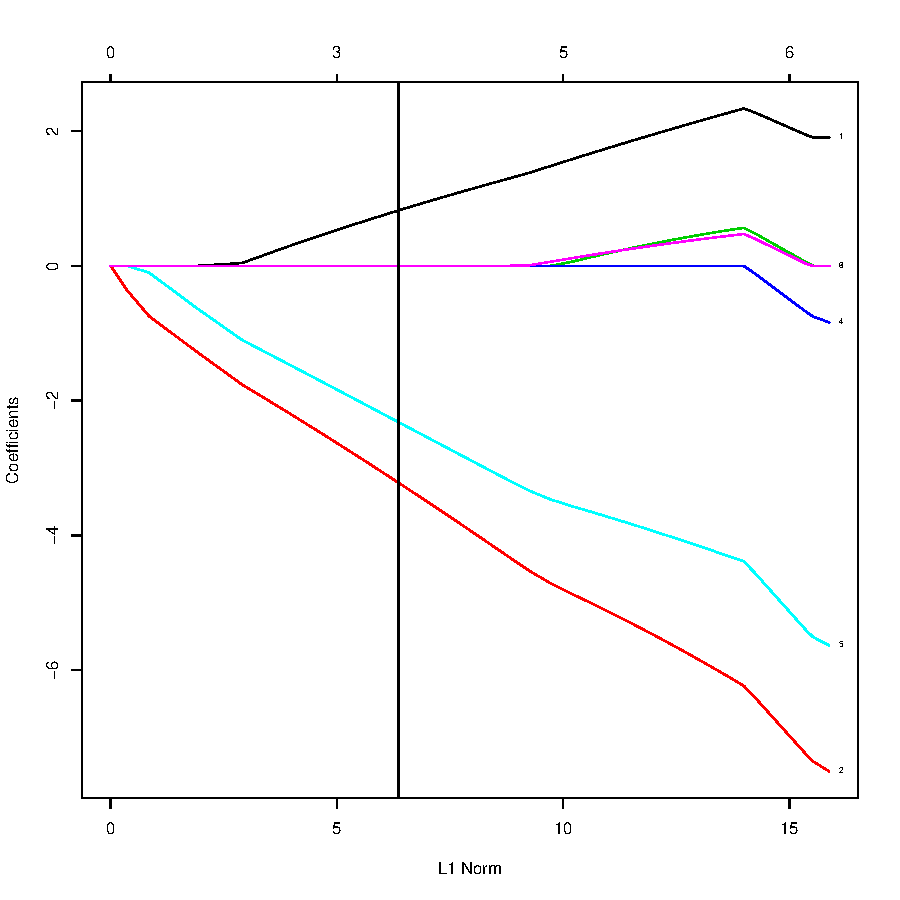
\includegraphics[width=\maxwidth]{figure/nmf-metagene-glmnet-plots-2} 

}


\begin{kframe}\begin{alltt}
\hlcom{# abline(v = sum(abs(coef(glmnet.fit.cv.diag_dsd$glmnet.fit, s =}
\hlcom{# glmnet.fit.cv.diag_dsd$lambda.min))))}
\hlkwd{coef}\hlstd{(glmnet.fit.cv.diag_dsd}\hlopt{$}\hlstd{glmnet.fit,} \hlkwc{s} \hlstd{= glmnet.fit.cv.diag_dsd}\hlopt{$}\hlstd{lambda.1se)}
\end{alltt}
\begin{verbatim}
## 6 x 1 sparse Matrix of class "dgCMatrix"
##          1
## V1  0.8238
## V2 -3.2195
## V3  .     
## V4  .     
## V5 -2.3208
## V6  .
\end{verbatim}
\begin{alltt}
\hlkwd{plot}\hlstd{(glmnet.fit.cv.diag_rec)}
\end{alltt}
\end{kframe}

{\centering 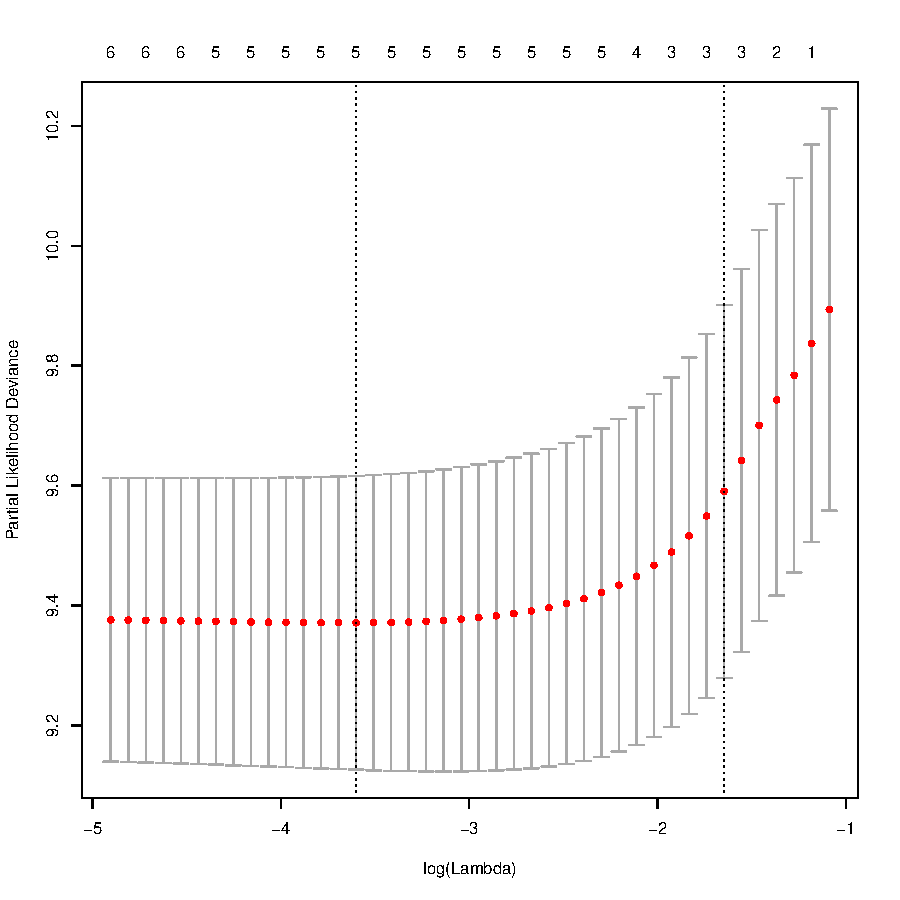
\includegraphics[width=\maxwidth]{figure/nmf-metagene-glmnet-plots-3} 

}


\begin{kframe}\begin{alltt}
\hlkwd{plot}\hlstd{(glmnet.fit.cv.diag_rec}\hlopt{$}\hlstd{glmnet.fit,} \hlkwc{label} \hlstd{=} \hlnum{TRUE}\hlstd{)}
\hlkwd{abline}\hlstd{(}\hlkwc{v} \hlstd{=} \hlkwd{sum}\hlstd{(}\hlkwd{abs}\hlstd{(}\hlkwd{coef}\hlstd{(glmnet.fit.cv.diag_rec}\hlopt{$}\hlstd{glmnet.fit,} \hlkwc{s} \hlstd{= glmnet.fit.cv.diag_rec}\hlopt{$}\hlstd{lambda.1se))))}
\end{alltt}
\end{kframe}

{\centering 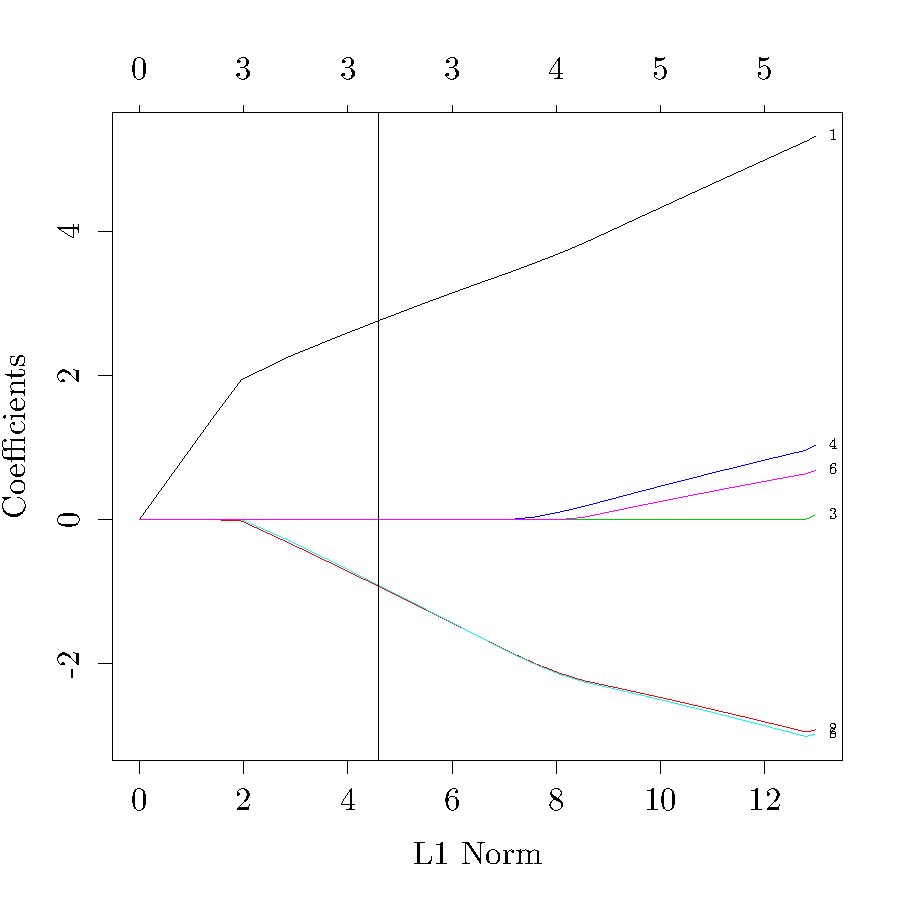
\includegraphics[width=\maxwidth]{figure/nmf-metagene-glmnet-plots-4} 

}


\begin{kframe}\begin{alltt}
\hlcom{# abline(v = sum(abs(coef(glmnet.fit.cv.diag_rec$glmnet.fit, s =}
\hlcom{# glmnet.fit.cv.diag_rec$lambda.min))))}
\hlkwd{coef}\hlstd{(glmnet.fit.cv.diag_rec}\hlopt{$}\hlstd{glmnet.fit,} \hlkwc{s} \hlstd{= glmnet.fit.cv.diag_rec}\hlopt{$}\hlstd{lambda.1se)}
\end{alltt}
\begin{verbatim}
## 6 x 1 sparse Matrix of class "dgCMatrix"
##          1
## V1  2.7555
## V2 -0.9230
## V3  .     
## V4  .     
## V5 -0.9055
## V6  .
\end{verbatim}
\begin{alltt}
\hlkwd{plot}\hlstd{(glmnet.fit.cv.recr_dsd)}
\end{alltt}
\end{kframe}

{\centering 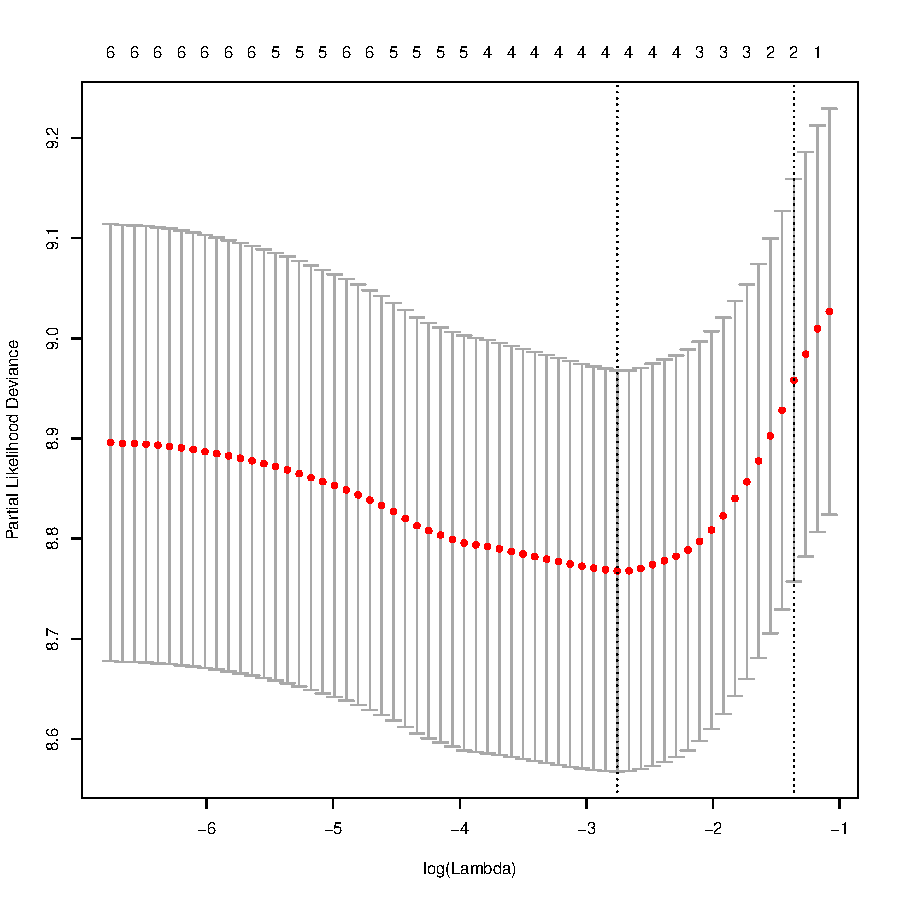
\includegraphics[width=\maxwidth]{figure/nmf-metagene-glmnet-plots-5} 

}


\begin{kframe}\begin{alltt}
\hlkwd{plot}\hlstd{(glmnet.fit.cv.recr_dsd}\hlopt{$}\hlstd{glmnet.fit,} \hlkwc{label} \hlstd{=} \hlnum{TRUE}\hlstd{)}
\hlkwd{abline}\hlstd{(}\hlkwc{v} \hlstd{=} \hlkwd{sum}\hlstd{(}\hlkwd{abs}\hlstd{(}\hlkwd{coef}\hlstd{(glmnet.fit.cv.recr_dsd}\hlopt{$}\hlstd{glmnet.fit,} \hlkwc{s} \hlstd{= glmnet.fit.cv.recr_dsd}\hlopt{$}\hlstd{lambda.1se))))}
\end{alltt}
\end{kframe}

{\centering 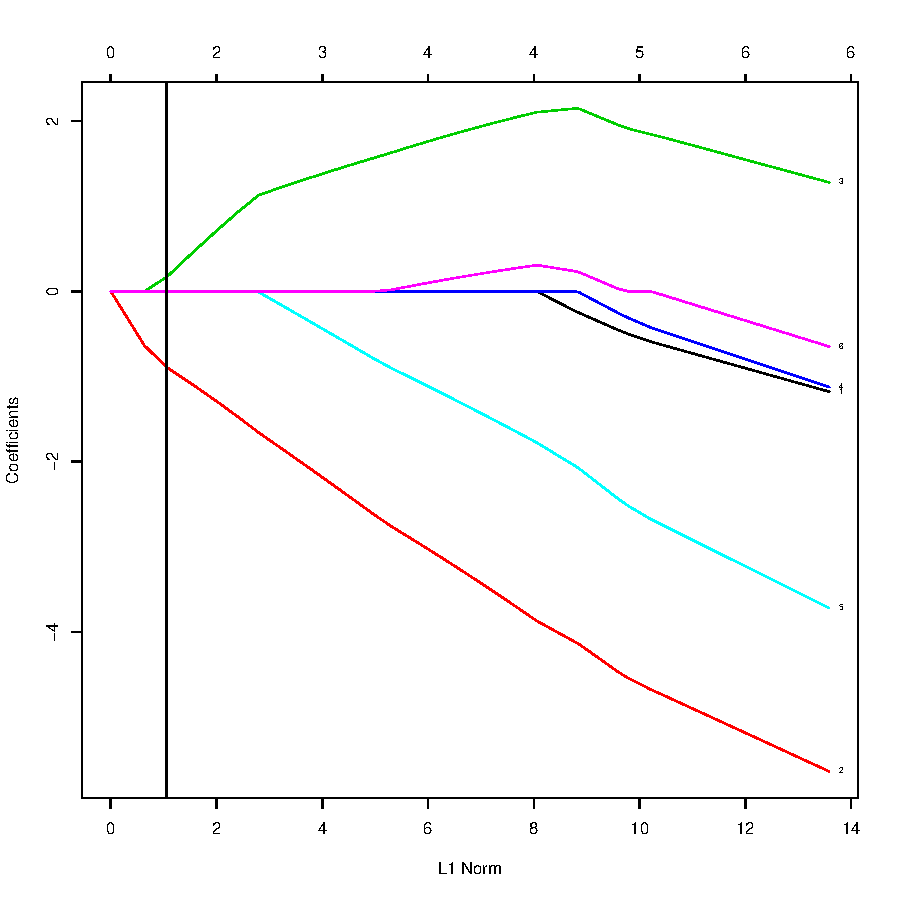
\includegraphics[width=\maxwidth]{figure/nmf-metagene-glmnet-plots-6} 

}


\begin{kframe}\begin{alltt}
\hlcom{# abline(v = sum(abs(coef(glmnet.fit.cv.recr_dsd$glmnet.fit, s =}
\hlcom{# glmnet.fit.cv.recr_dsd$lambda.min))))}
\hlkwd{coef}\hlstd{(glmnet.fit.cv.recr_dsd}\hlopt{$}\hlstd{glmnet.fit,} \hlkwc{s} \hlstd{= glmnet.fit.cv.recr_dsd}\hlopt{$}\hlstd{lambda.1se)}
\end{alltt}
\begin{verbatim}
## 6 x 1 sparse Matrix of class "dgCMatrix"
##          1
## V1  .     
## V2 -0.8920
## V3  0.1676
## V4  .     
## V5  .     
## V6  .
\end{verbatim}
\end{kframe}
\end{knitrout}


%%%%%%%%%%%%%%%%%%%%%%%%%%%%%%%%%%%%%%%%%%%%%%%%%%%%%%%%%%%%%%%%%%%%%%
% SIGNATURE PROGNOSTIC PERFORMANCE: CROSS-VALIDATION
%%%%%%%%%%%%%%%%%%%%%%%%%%%%%%%%%%%%%%%%%%%%%%%%%%%%%%%%%%%%%%%%%%%%%%
% \subsection{Prediction on 10-fold CV}
% <<cv-sig-load>>=
% cv_preds = readRDS("../../analysis/14_SIS_NMF_CV_results.rds")
% @

% <<cv-sig-test-alone>>=
% summary(coxph(y.diag_dsd ~ cv_preds["lasso.1se",]))
% @


%%%%%%%%%%%%%%%%%%%%%%%%%%%%%%%%%%%%%%%%%%%%%%%%%%%%%%%%%%%%%%%%%%%%%%
% SIGNATURE PROGNOSTIC PERFORMANCE: EXTERNAL VALIDATION
%%%%%%%%%%%%%%%%%%%%%%%%%%%%%%%%%%%%%%%%%%%%%%%%%%%%%%%%%%%%%%%%%%%%%%
\subsection{Prediction on validation sets}
\begin{knitrout}
\definecolor{shadecolor}{rgb}{0.969, 0.969, 0.969}\color{fgcolor}\begin{kframe}
\begin{alltt}
\hlkwd{load}\hlstd{(}\hlstr{"../../data/15_validation.rda"}\hlstd{)}
\end{alltt}
\end{kframe}
\end{knitrout}

\begin{knitrout}
\definecolor{shadecolor}{rgb}{0.969, 0.969, 0.969}\color{fgcolor}\begin{kframe}
\begin{alltt}
\hlstd{val.basis} \hlkwb{=} \hlkwd{basis}\hlstd{(nmf.final)}
\hlkwd{rownames}\hlstd{(GSE21501.lingex)} \hlkwb{=} \hlstd{GSE21501.feat}\hlopt{$}\hlstd{Gene.symbol}
\hlkwd{rownames}\hlstd{(GSE28735.lingex)} \hlkwb{=} \hlstd{GSE28735.feat}\hlopt{$}\hlstd{Gene.symbol}
\hlstd{GSE21501.lingex.for_basis} \hlkwb{=} \hlstd{GSE21501.lingex[}\hlkwd{match}\hlstd{(}\hlkwd{rownames}\hlstd{(val.basis),} \hlkwd{rownames}\hlstd{(GSE21501.lingex)),}
    \hlstd{]}
\hlstd{GSE28735.lingex.for_basis} \hlkwb{=} \hlstd{GSE28735.lingex[}\hlkwd{match}\hlstd{(}\hlkwd{rownames}\hlstd{(val.basis),} \hlkwd{rownames}\hlstd{(GSE28735.lingex)),}
    \hlstd{]}
\hlstd{GSE21501.lingex.for_basis[}\hlkwd{is.na}\hlstd{(GSE21501.lingex.for_basis)]} \hlkwb{=} \hlnum{0}
\hlstd{GSE28735.lingex.for_basis[}\hlkwd{is.na}\hlstd{(GSE28735.lingex.for_basis)]} \hlkwb{=} \hlnum{0}

\hlstd{GSE21501.coefs} \hlkwb{=} \hlkwd{apply}\hlstd{(GSE21501.lingex.for_basis,} \hlnum{2}\hlstd{,} \hlkwa{function}\hlstd{(}\hlkwc{xcol}\hlstd{)} \hlkwd{nnls}\hlstd{(val.basis,}
    \hlstd{xcol)}\hlopt{$}\hlstd{x)}
\hlstd{GSE28735.coefs} \hlkwb{=} \hlkwd{apply}\hlstd{(GSE28735.lingex.for_basis,} \hlnum{2}\hlstd{,} \hlkwa{function}\hlstd{(}\hlkwc{xcol}\hlstd{)} \hlkwd{nnls}\hlstd{(val.basis,}
    \hlstd{xcol)}\hlopt{$}\hlstd{x)}

\hlstd{GSE21501.axis1} \hlkwb{=} \hlstd{GSE21501.coefs[}\hlnum{1}\hlstd{, ]} \hlopt{-} \hlstd{GSE21501.coefs[}\hlnum{5}\hlstd{, ]}
\hlstd{GSE21501.axis2} \hlkwb{=} \hlstd{GSE21501.coefs[}\hlnum{6}\hlstd{, ]} \hlopt{-} \hlstd{GSE21501.coefs[}\hlnum{2}\hlstd{, ]}
\hlstd{GSE28735.axis1} \hlkwb{=} \hlstd{GSE28735.coefs[}\hlnum{1}\hlstd{, ]} \hlopt{-} \hlstd{GSE28735.coefs[}\hlnum{5}\hlstd{, ]}
\hlstd{GSE28735.axis2} \hlkwb{=} \hlstd{GSE28735.coefs[}\hlnum{6}\hlstd{, ]} \hlopt{-} \hlstd{GSE28735.coefs[}\hlnum{2}\hlstd{, ]}

\hlstd{GSE21501.score} \hlkwb{=} \hlnum{1.354} \hlopt{*} \hlstd{GSE21501.axis1} \hlopt{+} \hlnum{1.548} \hlopt{*} \hlstd{GSE21501.axis2}
\hlstd{GSE28735.score} \hlkwb{=} \hlnum{1.354} \hlopt{*} \hlstd{GSE28735.axis1} \hlopt{+} \hlnum{1.548} \hlopt{*} \hlstd{GSE28735.axis2}

\hlstd{GSE21501.pcna} \hlkwb{=} \hlkwd{apply}\hlstd{(GSE21501.gex[}\hlkwd{match}\hlstd{(metapcna.sig, GSE21501.feat}\hlopt{$}\hlstd{Gene.symbol),}
    \hlstd{],} \hlnum{2}\hlstd{, median,} \hlkwc{na.rm} \hlstd{=} \hlnum{TRUE}\hlstd{)}
\hlstd{GSE28735.pcna} \hlkwb{=} \hlkwd{apply}\hlstd{(GSE28735.gex[}\hlkwd{match}\hlstd{(metapcna.sig, GSE28735.feat}\hlopt{$}\hlstd{Gene.symbol),}
    \hlstd{],} \hlnum{2}\hlstd{, median,} \hlkwc{na.rm} \hlstd{=} \hlnum{TRUE}\hlstd{)}
\end{alltt}
\end{kframe}
\end{knitrout}

\begin{knitrout}
\definecolor{shadecolor}{rgb}{0.969, 0.969, 0.969}\color{fgcolor}\begin{kframe}
\begin{alltt}
\hlstd{temp} \hlkwb{=} \hlkwd{coxph}\hlstd{(}\hlkwd{Surv}\hlstd{(GSE21501.samp}\hlopt{$}\hlstd{time, GSE21501.samp}\hlopt{$}\hlstd{event)} \hlopt{~} \hlstd{GSE21501.score)}
\hlkwd{summary}\hlstd{(temp)}
\end{alltt}
\begin{verbatim}
## Call:
## coxph(formula = Surv(GSE21501.samp$time, GSE21501.samp$event) ~ 
##     GSE21501.score)
## 
##   n= 102, number of events= 66 
## 
##                coef exp(coef) se(coef)    z Pr(>|z|)
## GSE21501.score 1.81      6.13     1.14 1.59     0.11
## 
##                exp(coef) exp(-coef) lower .95 upper .95
## GSE21501.score      6.13      0.163     0.655      57.3
## 
## Concordance= 0.577  (se = 0.042 )
## Rsquare= 0.024   (max possible= 0.993 )
## Likelihood ratio test= 2.49  on 1 df,   p=0.115
## Wald test            = 2.52  on 1 df,   p=0.112
## Score (logrank) test = 2.54  on 1 df,   p=0.111
\end{verbatim}
\begin{alltt}
\hlstd{temp} \hlkwb{=} \hlkwd{coxph}\hlstd{(}\hlkwd{Surv}\hlstd{(GSE28735.samp}\hlopt{$}\hlstd{time, GSE28735.samp}\hlopt{$}\hlstd{event)} \hlopt{~} \hlstd{GSE28735.score)}
\hlkwd{summary}\hlstd{(temp)}
\end{alltt}
\begin{verbatim}
## Call:
## coxph(formula = Surv(GSE28735.samp$time, GSE28735.samp$event) ~ 
##     GSE28735.score)
## 
##   n= 42, number of events= 29 
## 
##                 coef exp(coef) se(coef)    z Pr(>|z|)
## GSE28735.score 1.867     6.471    0.752 2.48    0.013
## 
##                exp(coef) exp(-coef) lower .95 upper .95
## GSE28735.score      6.47      0.155      1.48      28.2
## 
## Concordance= 0.655  (se = 0.064 )
## Rsquare= 0.132   (max possible= 0.981 )
## Likelihood ratio test= 5.92  on 1 df,   p=0.0149
## Wald test            = 6.17  on 1 df,   p=0.013
## Score (logrank) test = 6.46  on 1 df,   p=0.011
\end{verbatim}
\begin{alltt}
\hlkwd{anova}\hlstd{(}\hlkwd{coxph}\hlstd{(}\hlkwd{Surv}\hlstd{(GSE21501.samp}\hlopt{$}\hlstd{time, GSE21501.samp}\hlopt{$}\hlstd{event)} \hlopt{~} \hlstd{GSE21501.axis1} \hlopt{+}
    \hlstd{GSE21501.axis2))}
\end{alltt}
\begin{verbatim}
## Analysis of Deviance Table
##  Cox model: response is Surv(GSE21501.samp$time, GSE21501.samp$event)
## Terms added sequentially (first to last)
## 
##                loglik Chisq Df Pr(>|Chi|)
## NULL             -255                    
## GSE21501.axis1   -254  1.44  1       0.23
## GSE21501.axis2   -254  1.09  1       0.30
\end{verbatim}
\begin{alltt}
\hlkwd{anova}\hlstd{(}\hlkwd{coxph}\hlstd{(}\hlkwd{Surv}\hlstd{(GSE28735.samp}\hlopt{$}\hlstd{time, GSE28735.samp}\hlopt{$}\hlstd{event)} \hlopt{~} \hlstd{GSE28735.axis1} \hlopt{+}
    \hlstd{GSE28735.axis2))}
\end{alltt}
\begin{verbatim}
## Analysis of Deviance Table
##  Cox model: response is Surv(GSE28735.samp$time, GSE28735.samp$event)
## Terms added sequentially (first to last)
## 
##                loglik Chisq Df Pr(>|Chi|)
## NULL            -83.1                    
## GSE28735.axis1  -81.4  3.43  1      0.064
## GSE28735.axis2  -80.2  2.51  1      0.113
\end{verbatim}
\end{kframe}
\end{knitrout}


\begin{knitrout}
\definecolor{shadecolor}{rgb}{0.969, 0.969, 0.969}\color{fgcolor}\begin{kframe}
\begin{alltt}
\hlkwd{load}\hlstd{(}\hlstr{"../../data/validation/tcga-clin-gex.20141118.rda"}\hlstd{)}
\end{alltt}
\end{kframe}
\end{knitrout}

\begin{knitrout}
\definecolor{shadecolor}{rgb}{0.969, 0.969, 0.969}\color{fgcolor}\begin{kframe}
\begin{alltt}
\hlstd{doValForSingleCancer} \hlkwb{=} \hlkwa{function}\hlstd{(}\hlkwc{cancer_id}\hlstd{) \{}
    \hlcom{# nevents, ntotal, score_p, anova_pcna, anova_score, anova_axis1,}
    \hlcom{# anova_axis2}
    \hlkwd{message}\hlstd{(cancer_id)}
    \hlstd{cancer_data} \hlkwb{=} \hlstd{data.merged[[cancer_id]]}
    \hlkwa{if} \hlstd{(}\hlopt{!}\hlstr{"illuminahiseq_rnaseqv2"} \hlopt \hlkwd{names}\hlstd{(cancer_data}\hlopt{$}\hlstd{gex)) \{}
        \hlkwd{return}\hlstd{(}\hlkwd{c}\hlstd{(}\hlnum{0}\hlstd{,} \hlnum{0}\hlstd{,} \hlnum{NA}\hlstd{,} \hlnum{NA}\hlstd{,} \hlnum{NA}\hlstd{,} \hlnum{NA}\hlstd{,} \hlnum{NA}\hlstd{))}
    \hlstd{\}}

    \hlstd{gex} \hlkwb{=} \hlstd{cancer_data}\hlopt{$}\hlstd{gex}\hlopt{$}\hlstd{illuminahiseq_rnaseqv2}
    \hlstd{clin} \hlkwb{=} \hlstd{cancer_data}\hlopt{$}\hlstd{clin}

    \hlstd{days_to_death} \hlkwb{=} \hlstd{clin}\hlopt{$}\hlstd{days_to_death}
    \hlstd{days_to_death[days_to_death} \hlopt{==} \hlstr{"[Not Applicable]"}\hlstd{]} \hlkwb{=} \hlnum{NA}
    \hlstd{days_to_death} \hlkwb{=} \hlkwd{as.numeric}\hlstd{(}\hlkwd{as.character}\hlstd{(days_to_death))}

    \hlstd{days_to_initial_pathologic_diagnosis} \hlkwb{=} \hlstd{clin}\hlopt{$}\hlstd{days_to_initial_pathologic_diagnosis}
    \hlstd{days_to_initial_pathologic_diagnosis[days_to_initial_pathologic_diagnosis} \hlopt{==}
        \hlstr{"[Not Applicable]"}\hlstd{]} \hlkwb{=} \hlnum{NA}
    \hlstd{days_to_initial_pathologic_diagnosis} \hlkwb{=} \hlkwd{as.numeric}\hlstd{(}\hlkwd{as.character}\hlstd{(days_to_initial_pathologic_diagnosis))}

    \hlstd{days_to_last_followup} \hlkwb{=} \hlstd{clin}\hlopt{$}\hlstd{days_to_last_followup}
    \hlstd{days_to_last_followup[days_to_last_followup} \hlopt{==} \hlstr{"[Not Applicable]"}\hlstd{]} \hlkwb{=} \hlnum{NA}
    \hlstd{days_to_last_followup} \hlkwb{=} \hlkwd{as.numeric}\hlstd{(}\hlkwd{as.character}\hlstd{(days_to_last_followup))}

    \hlstd{time_event} \hlkwb{=} \hlstd{days_to_death} \hlopt{-} \hlstd{days_to_initial_pathologic_diagnosis}
    \hlstd{time_lfu} \hlkwb{=} \hlstd{days_to_last_followup} \hlopt{-} \hlstd{days_to_initial_pathologic_diagnosis}
    \hlstd{time_obs} \hlkwb{=} \hlstd{time_event}
    \hlstd{time_obs[}\hlkwd{is.na}\hlstd{(time_obs)]} \hlkwb{=} \hlstd{time_lfu[}\hlkwd{is.na}\hlstd{(time_obs)]}
    \hlstd{time_obs[}\hlopt{!}\hlkwd{is.na}\hlstd{(time_obs)} \hlopt{& !}\hlkwd{is.na}\hlstd{(time_lfu)]} \hlkwb{=} \hlkwd{pmin}\hlstd{(time_obs[}\hlopt{!}\hlkwd{is.na}\hlstd{(time_obs)} \hlopt{&}
        \hlopt{!}\hlkwd{is.na}\hlstd{(time_lfu)], time_lfu[}\hlopt{!}\hlkwd{is.na}\hlstd{(time_obs)} \hlopt{& !}\hlkwd{is.na}\hlstd{(time_lfu)])}
    \hlstd{event} \hlkwb{=} \hlstd{(time_event} \hlopt{<=} \hlstd{time_lfu} \hlopt{& !}\hlkwd{is.na}\hlstd{(time_event)} \hlopt{& !}\hlkwd{is.na}\hlstd{(time_lfu))} \hlopt{|}
        \hlstd{(}\hlopt{!}\hlkwd{is.na}\hlstd{(time_event)} \hlopt{&} \hlkwd{is.na}\hlstd{(time_lfu))}

    \hlstd{y} \hlkwb{=} \hlkwd{Surv}\hlstd{(time_obs, event)}

    \hlstd{gex} \hlkwb{=} \hlstd{gex[}\hlopt{!}\hlkwd{grepl}\hlstd{(}\hlstr{"^\textbackslash{}\textbackslash{}?\textbackslash{}\textbackslash{}|"}\hlstd{,} \hlkwd{rownames}\hlstd{(gex)), ]}
    \hlkwd{rownames}\hlstd{(gex)} \hlkwb{=} \hlkwd{gsub}\hlstd{(}\hlstr{"\textbackslash{}\textbackslash{}|.*"}\hlstd{,} \hlstr{""}\hlstd{,} \hlkwd{rownames}\hlstd{(gex))}

    \hlstd{pcna} \hlkwb{=} \hlkwd{apply}\hlstd{(}\hlkwd{log2}\hlstd{(gex[}\hlkwd{rownames}\hlstd{(gex)} \hlopt \hlstd{metapcna.sig, ]} \hlopt{+} \hlnum{1}\hlstd{),} \hlnum{2}\hlstd{, median)}

    \hlstd{gex.axes} \hlkwb{=} \hlstd{gex[}\hlkwd{match}\hlstd{(}\hlkwd{rownames}\hlstd{(val.basis),} \hlkwd{rownames}\hlstd{(gex)), ]}
    \hlstd{gex.axes[}\hlkwd{apply}\hlstd{(}\hlkwd{is.na}\hlstd{(gex.axes),} \hlnum{1}\hlstd{, all), ]} \hlkwb{=} \hlnum{0}
    \hlstd{gex.axes} \hlkwb{=} \hlstd{gex.axes} \hlopt{-} \hlkwd{apply}\hlstd{(gex.axes,} \hlnum{1}\hlstd{, min,} \hlkwc{na.rm} \hlstd{=} \hlnum{TRUE}\hlstd{)}
    \hlstd{gex.axes} \hlkwb{=} \hlstd{gex.axes}\hlopt{/}\hlkwd{apply}\hlstd{(gex.axes,} \hlnum{1}\hlstd{, max,} \hlkwc{na.rm} \hlstd{=} \hlnum{TRUE}\hlstd{)}
    \hlstd{gex.axes[}\hlkwd{is.na}\hlstd{(gex.axes)]} \hlkwb{=} \hlnum{0}

    \hlstd{coefs} \hlkwb{=} \hlkwd{apply}\hlstd{(gex.axes,} \hlnum{2}\hlstd{,} \hlkwa{function}\hlstd{(}\hlkwc{xcol}\hlstd{)} \hlkwd{nnls}\hlstd{(val.basis, xcol)}\hlopt{$}\hlstd{x)}

    \hlstd{axis1} \hlkwb{=} \hlstd{coefs[}\hlnum{1}\hlstd{, ]} \hlopt{-} \hlstd{coefs[}\hlnum{5}\hlstd{, ]}
    \hlstd{axis2} \hlkwb{=} \hlstd{coefs[}\hlnum{6}\hlstd{, ]} \hlopt{-} \hlstd{coefs[}\hlnum{2}\hlstd{, ]}
    \hlstd{score} \hlkwb{=} \hlnum{1.354} \hlopt{*} \hlstd{axis1} \hlopt{+} \hlnum{1.548} \hlopt{*} \hlstd{axis2}

    \hlstd{valid} \hlkwb{=} \hlopt{!}\hlkwd{is.na}\hlstd{(score)} \hlopt{& !}\hlkwd{is.na}\hlstd{(pcna)} \hlopt{& !}\hlkwd{is.na}\hlstd{(y[,} \hlnum{1}\hlstd{])} \hlopt{& !}\hlkwd{is.na}\hlstd{(y[,} \hlnum{2}\hlstd{])}
    \hlstd{axis1} \hlkwb{=} \hlstd{axis1[valid]}
    \hlstd{axis2} \hlkwb{=} \hlstd{axis2[valid]}
    \hlstd{score} \hlkwb{=} \hlstd{score[valid]}
    \hlstd{pcna} \hlkwb{=} \hlstd{pcna[valid]}
    \hlstd{y} \hlkwb{=} \hlstd{y[valid, ]}

    \hlstd{nevents} \hlkwb{=} \hlkwd{sum}\hlstd{(y[,} \hlnum{2}\hlstd{])}
    \hlstd{ntotal} \hlkwb{=} \hlkwd{nrow}\hlstd{(y)}

    \hlstd{score_p} \hlkwb{=} \hlkwd{pchisq}\hlstd{(}\hlnum{2} \hlopt{*} \hlkwd{diff}\hlstd{(}\hlkwd{coxph}\hlstd{(y} \hlopt{~} \hlstd{score)}\hlopt{$}\hlstd{loglik),} \hlnum{1}\hlstd{,} \hlkwc{lower.tail} \hlstd{=} \hlnum{FALSE}\hlstd{)}
    \hlstd{anova_pcna} \hlkwb{=} \hlkwd{anova}\hlstd{(}\hlkwd{coxph}\hlstd{(y} \hlopt{~} \hlstd{pcna} \hlopt{+} \hlstd{score))[,} \hlstr{"Pr(>|Chi|)"}\hlstd{][}\hlnum{2}\hlstd{]}
    \hlstd{anova_score} \hlkwb{=} \hlkwd{anova}\hlstd{(}\hlkwd{coxph}\hlstd{(y} \hlopt{~} \hlstd{pcna} \hlopt{+} \hlstd{score))[,} \hlstr{"Pr(>|Chi|)"}\hlstd{][}\hlnum{3}\hlstd{]}
    \hlstd{anova_axis1} \hlkwb{=} \hlkwd{anova}\hlstd{(}\hlkwd{coxph}\hlstd{(y} \hlopt{~} \hlstd{axis1} \hlopt{+} \hlstd{axis2))[,} \hlstr{"Pr(>|Chi|)"}\hlstd{][}\hlnum{2}\hlstd{]}
    \hlstd{anova_axis2} \hlkwb{=} \hlkwd{anova}\hlstd{(}\hlkwd{coxph}\hlstd{(y} \hlopt{~} \hlstd{axis1} \hlopt{+} \hlstd{axis2))[,} \hlstr{"Pr(>|Chi|)"}\hlstd{][}\hlnum{3}\hlstd{]}

    \hlkwd{c}\hlstd{(nevents, ntotal, score_p, anova_pcna, anova_score, anova_axis1, anova_axis2)}
\hlstd{\}}


\hlstd{val_pvals} \hlkwb{=} \hlkwd{sapply}\hlstd{(}\hlkwd{names}\hlstd{(data.merged), doValForSingleCancer)}
\end{alltt}


{\ttfamily\noindent\itshape\color{messagecolor}{\#\# acc\\\#\# blca}}

{\ttfamily\noindent\color{warningcolor}{\#\# Warning in FUN(c("{}acc"{}, "{}blca"{}, "{}brca"{}, "{}cesc"{}, "{}coad"{}, "{}dlbc"{}, "{}gbm"{}, "{}hnsc"{}, : NAs introduced by coercion}}

{\ttfamily\noindent\color{warningcolor}{\#\# Warning in FUN(c("{}acc"{}, "{}blca"{}, "{}brca"{}, "{}cesc"{}, "{}coad"{}, "{}dlbc"{}, "{}gbm"{}, "{}hnsc"{}, : NAs introduced by coercion}}

{\ttfamily\noindent\color{warningcolor}{\#\# Warning in FUN(c("{}acc"{}, "{}blca"{}, "{}brca"{}, "{}cesc"{}, "{}coad"{}, "{}dlbc"{}, "{}gbm"{}, "{}hnsc"{}, : NAs introduced by coercion}}

{\ttfamily\noindent\itshape\color{messagecolor}{\#\# brca\\\#\# cesc\\\#\# coad\\\#\# dlbc}}

{\ttfamily\noindent\color{warningcolor}{\#\# Warning in fitter(X, Y, strats, offset, init, control, weights = weights, : Loglik converged before variable\ \ 1,2 ; beta may be infinite.}}

{\ttfamily\noindent\color{warningcolor}{\#\# Warning in fitter(X, Y, strats, offset, init, control, weights = weights, : Loglik converged before variable\ \ 1,2 ; beta may be infinite.}}

{\ttfamily\noindent\itshape\color{messagecolor}{\#\# gbm\\\#\# hnsc\\\#\# kich\\\#\# kirc\\\#\# kirp}}

{\ttfamily\noindent\color{warningcolor}{\#\# Warning in FUN(c("{}acc"{}, "{}blca"{}, "{}brca"{}, "{}cesc"{}, "{}coad"{}, "{}dlbc"{}, "{}gbm"{}, "{}hnsc"{}, : NAs introduced by coercion}}

{\ttfamily\noindent\itshape\color{messagecolor}{\#\# lgg}}

{\ttfamily\noindent\color{warningcolor}{\#\# Warning in FUN(c("{}acc"{}, "{}blca"{}, "{}brca"{}, "{}cesc"{}, "{}coad"{}, "{}dlbc"{}, "{}gbm"{}, "{}hnsc"{}, : NAs introduced by coercion}}

{\ttfamily\noindent\itshape\color{messagecolor}{\#\# lihc\\\#\# luad}}

{\ttfamily\noindent\color{warningcolor}{\#\# Warning in FUN(c("{}acc"{}, "{}blca"{}, "{}brca"{}, "{}cesc"{}, "{}coad"{}, "{}dlbc"{}, "{}gbm"{}, "{}hnsc"{}, : NAs introduced by coercion}}

{\ttfamily\noindent\itshape\color{messagecolor}{\#\# lusc}}

{\ttfamily\noindent\color{warningcolor}{\#\# Warning in FUN(c("{}acc"{}, "{}blca"{}, "{}brca"{}, "{}cesc"{}, "{}coad"{}, "{}dlbc"{}, "{}gbm"{}, "{}hnsc"{}, : NAs introduced by coercion}}

{\ttfamily\noindent\itshape\color{messagecolor}{\#\# meso\\\#\# ov\\\#\# paad\\\#\# prad}}

{\ttfamily\noindent\color{warningcolor}{\#\# Warning in fitter(X, Y, strats, offset, init, control, weights = weights, : Ran out of iterations and did not converge}}

{\ttfamily\noindent\color{warningcolor}{\#\# Warning in fitter(X, Y, strats, offset, init, control, weights = weights, : Ran out of iterations and did not converge}}

{\ttfamily\noindent\itshape\color{messagecolor}{\#\# read\\\#\# sarc\\\#\# skcm}}

{\ttfamily\noindent\color{warningcolor}{\#\# Warning in FUN(c("{}acc"{}, "{}blca"{}, "{}brca"{}, "{}cesc"{}, "{}coad"{}, "{}dlbc"{}, "{}gbm"{}, "{}hnsc"{}, : NAs introduced by coercion}}

{\ttfamily\noindent\color{warningcolor}{\#\# Warning in FUN(c("{}acc"{}, "{}blca"{}, "{}brca"{}, "{}cesc"{}, "{}coad"{}, "{}dlbc"{}, "{}gbm"{}, "{}hnsc"{}, : NAs introduced by coercion}}

{\ttfamily\noindent\itshape\color{messagecolor}{\#\# thca\\\#\# ucec}}

{\ttfamily\noindent\color{warningcolor}{\#\# Warning in FUN(c("{}acc"{}, "{}blca"{}, "{}brca"{}, "{}cesc"{}, "{}coad"{}, "{}dlbc"{}, "{}gbm"{}, "{}hnsc"{}, : NAs introduced by coercion}}

{\ttfamily\noindent\color{warningcolor}{\#\# Warning in FUN(c("{}acc"{}, "{}blca"{}, "{}brca"{}, "{}cesc"{}, "{}coad"{}, "{}dlbc"{}, "{}gbm"{}, "{}hnsc"{}, : NAs introduced by coercion}}

{\ttfamily\noindent\itshape\color{messagecolor}{\#\# ucs}}\begin{alltt}
\hlkwd{rownames}\hlstd{(val_pvals)} \hlkwb{=} \hlkwd{c}\hlstd{(}\hlstr{"nevents"}\hlstd{,} \hlstr{"ntotal"}\hlstd{,} \hlstr{"p.score"}\hlstd{,} \hlstr{"p.anova.pcna"}\hlstd{,} \hlstr{"p.anova.pcna_score"}\hlstd{,}
    \hlstr{"p.anova.axis1"}\hlstd{,} \hlstr{"p.anova.axis1_axis2"}\hlstd{)}
\hlstd{val_pvals} \hlkwb{=} \hlkwd{as.data.frame}\hlstd{(}\hlkwd{t}\hlstd{(val_pvals))}

\hlstd{val_pvals[val_pvals}\hlopt{$}\hlstd{nevents} \hlopt{>=} \hlnum{50} \hlopt{|} \hlkwd{rownames}\hlstd{(val_pvals)} \hlopt{==} \hlstr{"paad"}\hlstd{, ]}
\end{alltt}
\begin{verbatim}
##      nevents ntotal   p.score p.anova.pcna p.anova.pcna_score
## gbm       54    143 2.287e-01    8.185e-01          0.1587102
## hnsc     124    367 8.075e-03    4.719e-01          0.0107907
## kirc     153    497 2.034e-12    9.569e-11          0.0028892
## lgg       53    272 1.493e-05    6.316e-04          0.0078542
## luad     106    431 8.336e-06    7.205e-03          0.0001042
## lusc     117    395 9.624e-01    7.035e-02          0.4109578
## ov       115    251 2.380e-02    5.903e-01          0.0178108
## paad      17     58 4.952e-03    8.549e-02          0.0239990
##      p.anova.axis1 p.anova.axis1_axis2
## gbm      9.252e-01           6.877e-02
## hnsc     4.367e-02           8.341e-02
## kirc     2.673e-08           1.639e-05
## lgg      1.593e-04           3.350e-02
## luad     1.238e-03           1.543e-03
## lusc     1.597e-01           2.559e-01
## ov       3.655e-01           3.298e-02
## paad     1.562e-02           1.249e-01
\end{verbatim}
\end{kframe}
\end{knitrout}


\begin{knitrout}
\definecolor{shadecolor}{rgb}{0.969, 0.969, 0.969}\color{fgcolor}\begin{kframe}
\begin{alltt}
\hlstd{plot_km_axes} \hlkwb{=} \hlkwa{function}\hlstd{(}\hlkwc{axis1}\hlstd{,} \hlkwc{axis2}\hlstd{,} \hlkwc{y}\hlstd{,} \hlkwc{mc} \hlstd{=} \hlnum{FALSE}\hlstd{,} \hlkwc{...}\hlstd{) \{}
    \hlstd{t1} \hlkwb{=} \hlstd{t2} \hlkwb{=} \hlnum{0}
    \hlkwa{if} \hlstd{(mc} \hlopt{==} \hlnum{TRUE}\hlstd{) \{}
        \hlstd{t1} \hlkwb{=} \hlkwd{median}\hlstd{(axis1,} \hlkwc{na.rm} \hlstd{=} \hlnum{TRUE}\hlstd{)}
        \hlstd{t2} \hlkwb{=} \hlkwd{median}\hlstd{(axis2,} \hlkwc{na.rm} \hlstd{=} \hlnum{TRUE}\hlstd{)}
    \hlstd{\}}

    \hlstd{class} \hlkwb{=} \hlkwd{paste}\hlstd{(}\hlkwd{c}\hlstd{(}\hlstr{"L"}\hlstd{,} \hlstr{"H"}\hlstd{)[}\hlkwd{I}\hlstd{(axis1} \hlopt{>=} \hlstd{t1)} \hlopt{+} \hlnum{1}\hlstd{],} \hlkwd{c}\hlstd{(}\hlstr{"L"}\hlstd{,} \hlstr{"H"}\hlstd{)[}\hlkwd{I}\hlstd{(axis2} \hlopt{>=} \hlstd{t2)} \hlopt{+}
        \hlnum{1}\hlstd{],} \hlkwc{sep} \hlstd{=} \hlstr{""}\hlstd{)}
    \hlstd{class} \hlkwb{=} \hlkwd{ordered}\hlstd{(class,} \hlkwc{levels} \hlstd{=} \hlkwd{c}\hlstd{(}\hlstr{"LL"}\hlstd{,} \hlstr{"LH"}\hlstd{,} \hlstr{"HL"}\hlstd{,} \hlstr{"HH"}\hlstd{))}
    \hlstd{fit} \hlkwb{=} \hlkwd{survfit}\hlstd{(y} \hlopt{~} \hlstd{class)}
    \hlkwd{print}\hlstd{(fit)}
    \hlkwd{print}\hlstd{(}\hlkwd{survdiff}\hlstd{(y} \hlopt{~} \hlstd{class))}
    \hlstd{pval} \hlkwb{=} \hlkwd{pchisq}\hlstd{(}\hlkwd{survdiff}\hlstd{(y} \hlopt{~} \hlstd{class)}\hlopt{$}\hlstd{chisq,} \hlnum{3}\hlstd{,} \hlkwc{lower.tail} \hlstd{=} \hlnum{FALSE}\hlstd{)}
    \hlstd{pal} \hlkwb{=} \hlkwd{brewer.pal}\hlstd{(}\hlnum{4}\hlstd{,} \hlstr{"Set2"}\hlstd{)}
    \hlkwd{names}\hlstd{(pal)} \hlkwb{=} \hlkwd{c}\hlstd{(}\hlstr{"LL"}\hlstd{,} \hlstr{"LH"}\hlstd{,} \hlstr{"HL"}\hlstd{,} \hlstr{"HH"}\hlstd{)}
    \hlkwd{plot}\hlstd{(axis2} \hlopt{~} \hlstd{axis1,} \hlkwc{xlab} \hlstd{=} \hlstr{"A1 activity"}\hlstd{,} \hlkwc{ylab} \hlstd{=} \hlstr{"A2 activity"}\hlstd{,} \hlkwc{col} \hlstd{= pal[class],}
        \hlkwc{pch} \hlstd{=} \hlnum{16}\hlstd{,} \hlkwc{cex} \hlstd{=} \hlnum{1.5}\hlstd{, ...)}
    \hlkwd{abline}\hlstd{(}\hlkwc{h} \hlstd{= t2)}
    \hlkwd{abline}\hlstd{(}\hlkwc{v} \hlstd{= t1)}
    \hlkwd{plot}\hlstd{(fit,} \hlkwc{col} \hlstd{= pal,} \hlkwc{lwd} \hlstd{=} \hlnum{2}\hlstd{,} \hlkwc{xlab} \hlstd{=} \hlstr{"Time from diagnosis (days)"}\hlstd{,} \hlkwc{ylab} \hlstd{=} \hlstr{"Fraction surviving"}\hlstd{,}
        \hlkwc{sub} \hlstd{=} \hlkwd{sprintf}\hlstd{(}\hlstr{"P = %.3g"}\hlstd{, pval), ...)}
\hlstd{\}}

\hlstd{plot_km_axes_tcga} \hlkwb{=} \hlkwa{function}\hlstd{(}\hlkwc{code}\hlstd{,} \hlkwc{mc}\hlstd{) \{}
    \hlkwa{if} \hlstd{(}\hlstr{"illuminahiseq_rnaseqv2"} \hlopt \hlkwd{names}\hlstd{(data.merged[[code]]}\hlopt{$}\hlstd{gex)) \{}
        \hlstd{temp.gex} \hlkwb{=} \hlstd{data.merged[[code]]}\hlopt{$}\hlstd{gex}\hlopt{$}\hlstd{illuminahiseq_rnaseqv2}
        \hlstd{temp.gex} \hlkwb{=} \hlstd{temp.gex[}\hlopt{!}\hlkwd{grepl}\hlstd{(}\hlstr{"^\textbackslash{}\textbackslash{}?\textbackslash{}\textbackslash{}|"}\hlstd{,} \hlkwd{rownames}\hlstd{(temp.gex)), ]}
        \hlkwd{rownames}\hlstd{(temp.gex)} \hlkwb{=} \hlkwd{gsub}\hlstd{(}\hlstr{"\textbackslash{}\textbackslash{}|.*"}\hlstd{,} \hlstr{""}\hlstd{,} \hlkwd{rownames}\hlstd{(temp.gex))}
        \hlstd{temp.gex.axes} \hlkwb{=} \hlstd{temp.gex[}\hlkwd{match}\hlstd{(}\hlkwd{rownames}\hlstd{(val.basis),} \hlkwd{rownames}\hlstd{(temp.gex)),}
            \hlstd{]}
        \hlstd{temp.gex.axes[}\hlkwd{apply}\hlstd{(}\hlkwd{is.na}\hlstd{(temp.gex.axes),} \hlnum{1}\hlstd{, all), ]} \hlkwb{=} \hlnum{0}
        \hlstd{temp.gex.axes} \hlkwb{=} \hlstd{temp.gex.axes} \hlopt{-} \hlkwd{apply}\hlstd{(temp.gex.axes,} \hlnum{1}\hlstd{, min,} \hlkwc{na.rm} \hlstd{=} \hlnum{TRUE}\hlstd{)}
        \hlstd{temp.gex.axes} \hlkwb{=} \hlstd{temp.gex.axes}\hlopt{/}\hlkwd{apply}\hlstd{(temp.gex.axes,} \hlnum{1}\hlstd{, max,} \hlkwc{na.rm} \hlstd{=} \hlnum{TRUE}\hlstd{)}
        \hlstd{temp.gex.axes[}\hlkwd{is.na}\hlstd{(temp.gex.axes)]} \hlkwb{=} \hlnum{0}
        \hlstd{temp.coefs} \hlkwb{=} \hlkwd{apply}\hlstd{(temp.gex.axes,} \hlnum{2}\hlstd{,} \hlkwa{function}\hlstd{(}\hlkwc{xcol}\hlstd{)} \hlkwd{nnls}\hlstd{(val.basis,}
            \hlstd{xcol)}\hlopt{$}\hlstd{x)}
        \hlstd{temp.axis1} \hlkwb{=} \hlstd{temp.coefs[}\hlnum{1}\hlstd{, ]} \hlopt{-} \hlstd{temp.coefs[}\hlnum{5}\hlstd{, ]}
        \hlstd{temp.axis2} \hlkwb{=} \hlstd{temp.coefs[}\hlnum{6}\hlstd{, ]} \hlopt{-} \hlstd{temp.coefs[}\hlnum{2}\hlstd{, ]}

        \hlstd{temp.clin} \hlkwb{=} \hlstd{data.merged[[code]]}\hlopt{$}\hlstd{clin}
        \hlstd{temp.days_to_death} \hlkwb{=} \hlstd{temp.clin}\hlopt{$}\hlstd{days_to_death}
        \hlstd{temp.days_to_death[temp.days_to_death} \hlopt{==} \hlstr{"[Not Applicable]"}\hlstd{]} \hlkwb{=} \hlnum{NA}
        \hlstd{temp.days_to_death} \hlkwb{=} \hlkwd{as.numeric}\hlstd{(}\hlkwd{as.character}\hlstd{(temp.days_to_death))}
        \hlstd{temp.days_to_initial_pathologic_diagnosis} \hlkwb{=} \hlstd{temp.clin}\hlopt{$}\hlstd{days_to_initial_pathologic_diagnosis}
        \hlstd{temp.days_to_initial_pathologic_diagnosis[temp.days_to_initial_pathologic_diagnosis} \hlopt{==}
            \hlstr{"[Not Applicable]"}\hlstd{]} \hlkwb{=} \hlnum{NA}
        \hlstd{temp.days_to_initial_pathologic_diagnosis} \hlkwb{=} \hlkwd{as.numeric}\hlstd{(}\hlkwd{as.character}\hlstd{(temp.days_to_initial_pathologic_diagnosis))}
        \hlstd{temp.days_to_last_followup} \hlkwb{=} \hlstd{temp.clin}\hlopt{$}\hlstd{days_to_last_followup}
        \hlstd{temp.days_to_last_followup[temp.days_to_last_followup} \hlopt{==} \hlstr{"[Not Applicable]"}\hlstd{]} \hlkwb{=} \hlnum{NA}
        \hlstd{temp.days_to_last_followup} \hlkwb{=} \hlkwd{as.numeric}\hlstd{(}\hlkwd{as.character}\hlstd{(temp.days_to_last_followup))}
        \hlstd{temp.time_event} \hlkwb{=} \hlstd{temp.days_to_death} \hlopt{-} \hlstd{temp.days_to_initial_pathologic_diagnosis}
        \hlstd{temp.time_lfu} \hlkwb{=} \hlstd{temp.days_to_last_followup} \hlopt{-} \hlstd{temp.days_to_initial_pathologic_diagnosis}
        \hlstd{temp.time_obs} \hlkwb{=} \hlstd{temp.time_event}
        \hlstd{temp.time_obs[}\hlkwd{is.na}\hlstd{(temp.time_obs)]} \hlkwb{=} \hlstd{temp.time_lfu[}\hlkwd{is.na}\hlstd{(temp.time_obs)]}
        \hlstd{temp.time_obs[}\hlopt{!}\hlkwd{is.na}\hlstd{(temp.time_obs)} \hlopt{& !}\hlkwd{is.na}\hlstd{(temp.time_lfu)]} \hlkwb{=} \hlkwd{pmin}\hlstd{(temp.time_obs[}\hlopt{!}\hlkwd{is.na}\hlstd{(temp.time_obs)} \hlopt{&}
            \hlopt{!}\hlkwd{is.na}\hlstd{(temp.time_lfu)], temp.time_lfu[}\hlopt{!}\hlkwd{is.na}\hlstd{(temp.time_obs)} \hlopt{& !}\hlkwd{is.na}\hlstd{(temp.time_lfu)])}
        \hlstd{temp.event} \hlkwb{=} \hlstd{(temp.time_event} \hlopt{<=} \hlstd{temp.time_lfu} \hlopt{& !}\hlkwd{is.na}\hlstd{(temp.time_event)} \hlopt{&}
            \hlopt{!}\hlkwd{is.na}\hlstd{(temp.time_lfu))} \hlopt{|} \hlstd{(}\hlopt{!}\hlkwd{is.na}\hlstd{(temp.time_event)} \hlopt{&} \hlkwd{is.na}\hlstd{(temp.time_lfu))}
        \hlstd{temp.y} \hlkwb{=} \hlkwd{Surv}\hlstd{(temp.time_obs, temp.event)}

        \hlkwd{plot_km_axes}\hlstd{(temp.axis1, temp.axis2, temp.y,} \hlkwc{mc} \hlstd{=} \hlnum{FALSE}\hlstd{,} \hlkwc{main} \hlstd{= code)}
    \hlstd{\}}
\hlstd{\}}

\hlkwd{plot_km_axes}\hlstd{(axis_coefs.diag_dsd[,} \hlnum{1}\hlstd{], axis_coefs.diag_dsd[,} \hlnum{2}\hlstd{], y.diag_dsd,}
    \hlkwc{mc} \hlstd{=} \hlnum{FALSE}\hlstd{,} \hlkwc{main} \hlstd{=} \hlstr{"APGI"}\hlstd{)}
\end{alltt}
\begin{verbatim}
## Call: survfit(formula = y ~ class)
## 
##          records n.max n.start events median 0.95LCL 0.95UCL
## class=LL      38    38      38     14     NA     913      NA
## class=LH      21    21      21     16    641     482      NA
## class=HL      23    23      23     15    970     709      NA
## class=HH      28    28      28     25    345     280     495
## Call:
## survdiff(formula = y ~ class)
## 
##           N Observed Expected (O-E)^2/E (O-E)^2/V
## class=LL 38       14    31.77     9.942    18.645
## class=LH 21       16    13.02     0.683     0.852
## class=HL 23       15    17.66     0.401     0.543
## class=HH 28       25     7.55    40.376    48.292
## 
##  Chisq= 55.7  on 3 degrees of freedom, p= 4.98e-12
\end{verbatim}
\end{kframe}

{\centering 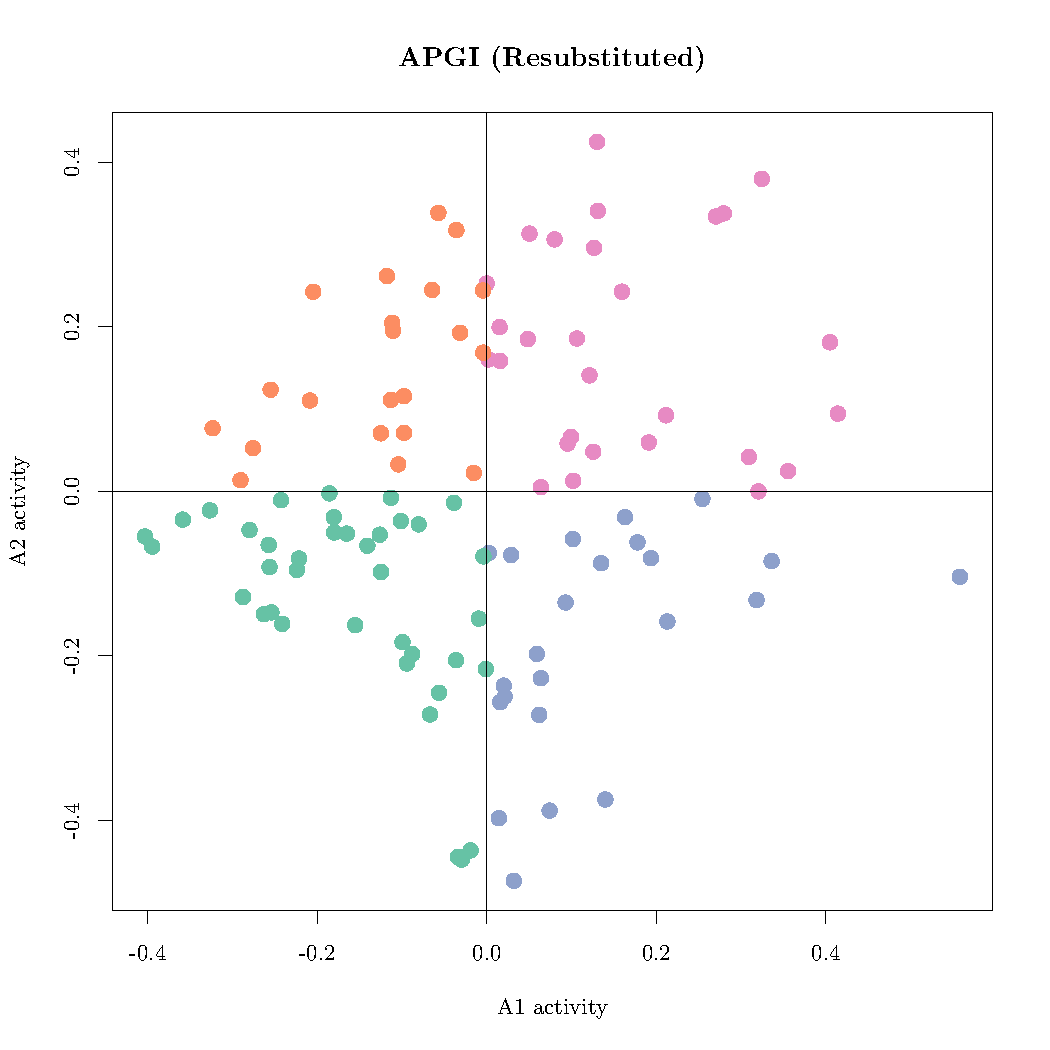
\includegraphics[width=\maxwidth]{figure/km-curves-1} 

}




{\centering 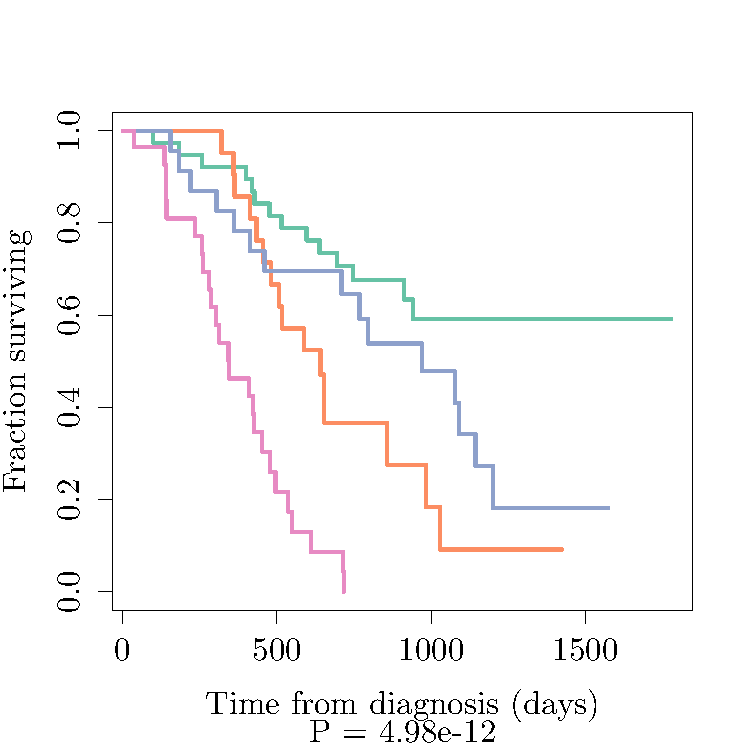
\includegraphics[width=\maxwidth]{figure/km-curves-2} 

}


\begin{kframe}\begin{alltt}
\hlkwd{plot_km_axes}\hlstd{(GSE21501.axis1, GSE21501.axis2,} \hlkwd{Surv}\hlstd{(GSE21501.samp}\hlopt{$}\hlstd{time, GSE21501.samp}\hlopt{$}\hlstd{event),}
    \hlkwc{mc} \hlstd{=} \hlnum{FALSE}\hlstd{,} \hlkwc{main} \hlstd{=} \hlstr{"GSE21501"}\hlstd{)}
\end{alltt}
\begin{verbatim}
## Call: survfit(formula = y ~ class)
## 
##          records n.max n.start events median 0.95LCL 0.95UCL
## class=LL      11    11      11      7     22       7      NA
## class=LH      50    50      50     33     19      15      25
## class=HL       5     5       5      4     14      14      NA
## class=HH      36    36      36     22     18      10      NA
## Call:
## survdiff(formula = y ~ class)
## 
##           N Observed Expected (O-E)^2/E (O-E)^2/V
## class=LL 11        7     8.12  1.56e-01  1.95e-01
## class=LH 50       33    32.96  3.96e-05  8.43e-05
## class=HL  5        4     3.91  2.27e-03  2.53e-03
## class=HH 36       22    21.01  4.71e-02  7.23e-02
## 
##  Chisq= 0.2  on 3 degrees of freedom, p= 0.974
\end{verbatim}
\end{kframe}

{\centering 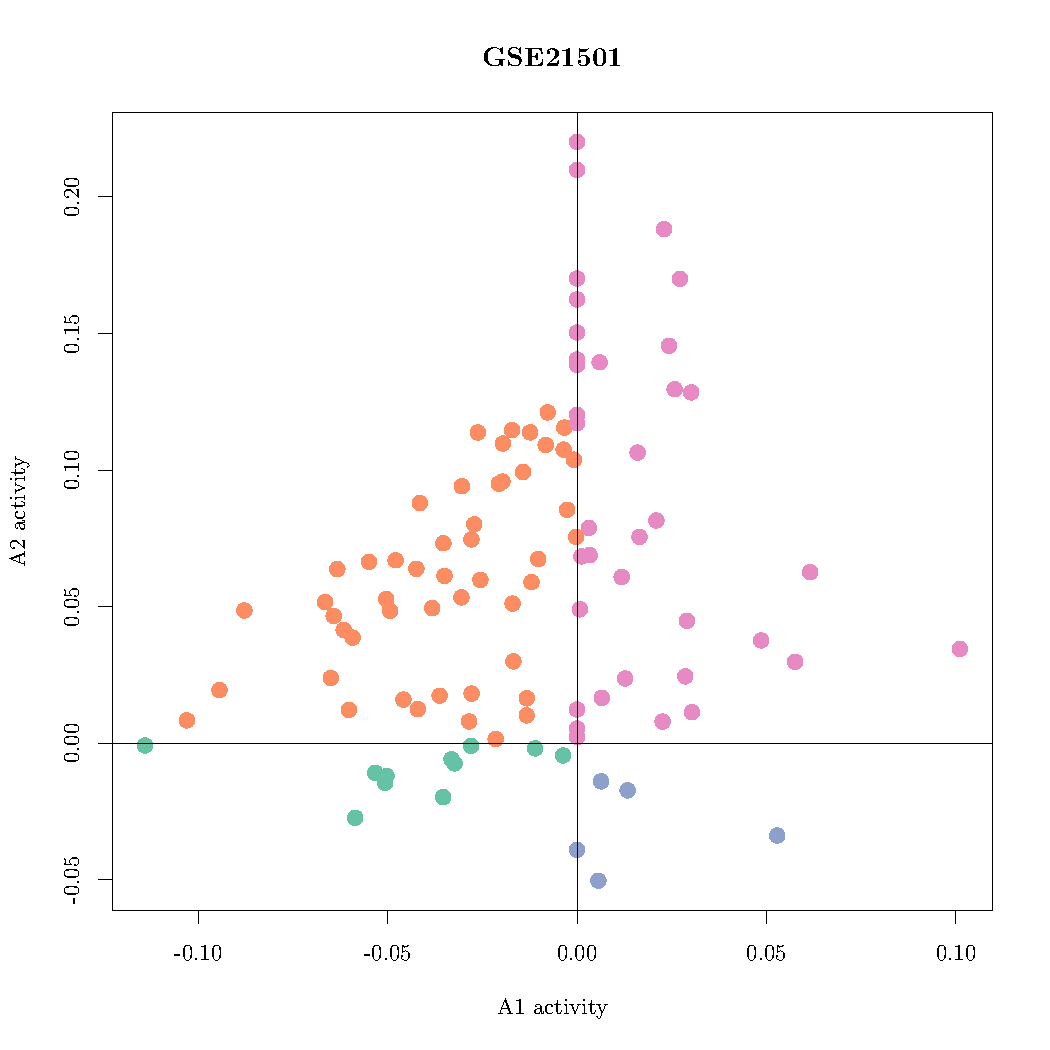
\includegraphics[width=\maxwidth]{figure/km-curves-3} 

}




{\centering 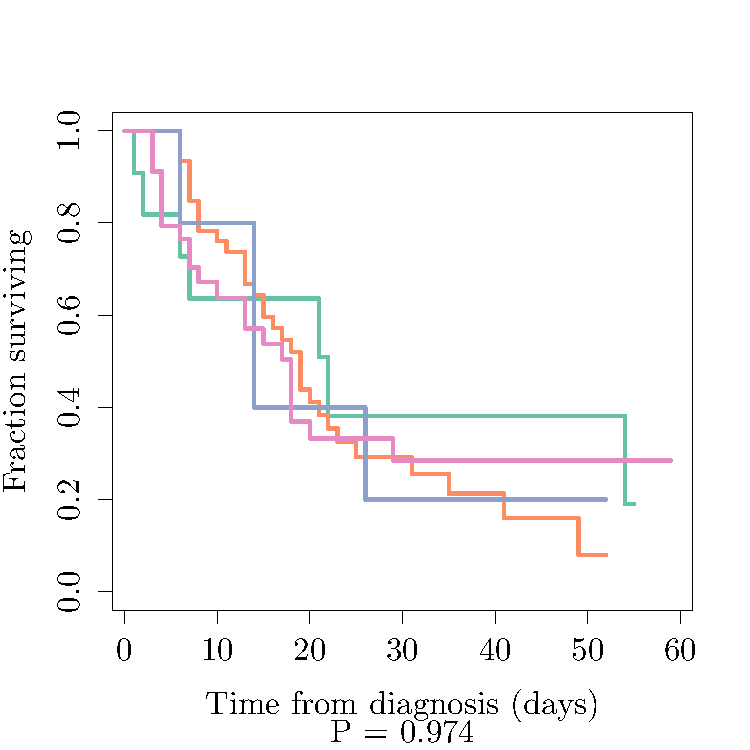
\includegraphics[width=\maxwidth]{figure/km-curves-4} 

}


\begin{kframe}\begin{alltt}
\hlkwd{plot_km_axes}\hlstd{(GSE28735.axis1, GSE28735.axis2,} \hlkwd{Surv}\hlstd{(GSE28735.samp}\hlopt{$}\hlstd{time, GSE28735.samp}\hlopt{$}\hlstd{event),}
    \hlkwc{mc} \hlstd{=} \hlnum{FALSE}\hlstd{,} \hlkwc{main} \hlstd{=} \hlstr{"GSE28735"}\hlstd{)}
\end{alltt}
\begin{verbatim}
## Call: survfit(formula = y ~ class)
## 
##          records n.max n.start events median 0.95LCL 0.95UCL
## class=LL       6     6       6      3     51      16      NA
## class=LH      13    13      13      9     25      13      NA
## class=HL       1     1       1      0     NA      NA      NA
## class=HH      22    22      22     17     13       8      NA
## Call:
## survdiff(formula = y ~ class)
## 
##           N Observed Expected (O-E)^2/E (O-E)^2/V
## class=LL  6        3    6.651     2.004     3.168
## class=LH 13        9   10.078     0.115     0.186
## class=HL  1        0    0.735     0.735     0.779
## class=HH 22       17   11.536     2.588     4.733
## 
##  Chisq= 6.2  on 3 degrees of freedom, p= 0.101
\end{verbatim}
\end{kframe}

{\centering 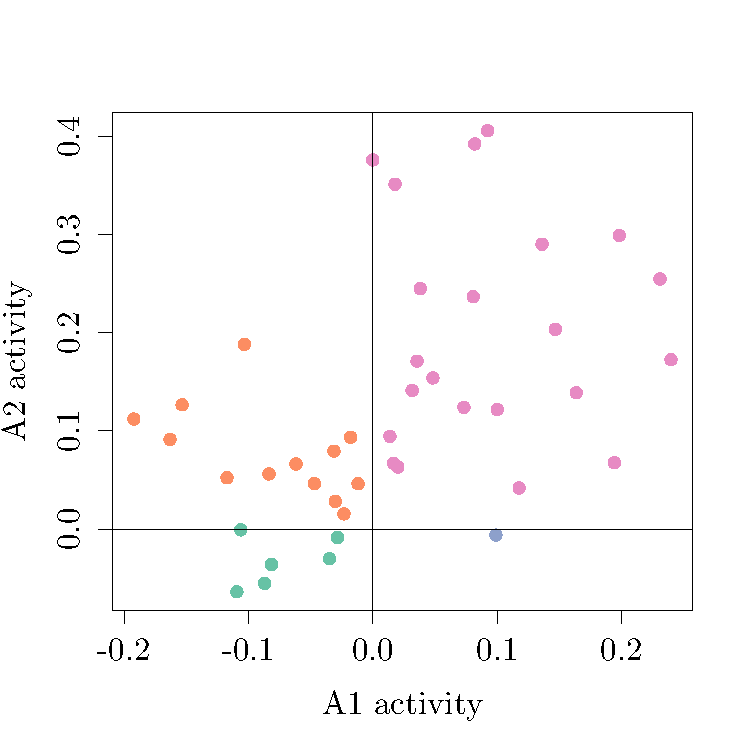
\includegraphics[width=\maxwidth]{figure/km-curves-5} 

}




{\centering 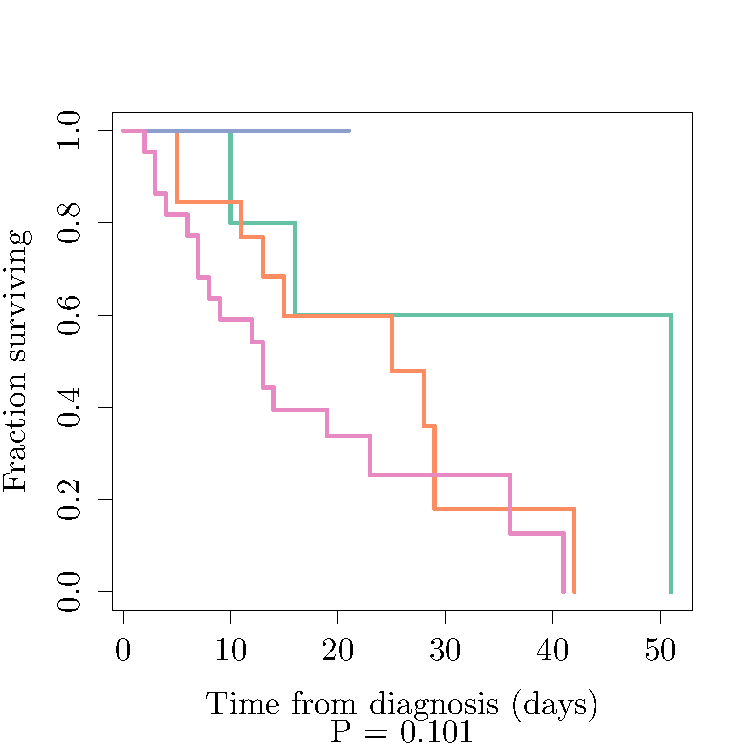
\includegraphics[width=\maxwidth]{figure/km-curves-6} 

}


\begin{kframe}\begin{alltt}
\hlkwd{plot_km_axes_tcga}\hlstd{(}\hlstr{"hnsc"}\hlstd{,} \hlkwc{mc} \hlstd{=} \hlnum{FALSE}\hlstd{)}
\end{alltt}
\begin{verbatim}
## Call: survfit(formula = y ~ class)
## 
##    1 observation deleted due to missingness 
##          records n.max n.start events median 0.95LCL 0.95UCL
## class=LL      11    11      11      3   1459     822      NA
## class=LH      43    43      43      8   2717    1591      NA
## class=HL      90    90      90     26   1748     914      NA
## class=HH     223   223     223     87   1037     669    2002
## Call:
## survdiff(formula = y ~ class)
## 
## n=367, 1 observation deleted due to missingness.
## 
##            N Observed Expected (O-E)^2/E (O-E)^2/V
## class=LL  11        3     3.77     0.156     0.162
## class=LH  43        8    15.60     3.700     4.249
## class=HL  90       26    29.68     0.457     0.606
## class=HH 223       87    74.95     1.936     4.969
## 
##  Chisq= 6.3  on 3 degrees of freedom, p= 0.0969
\end{verbatim}
\end{kframe}

{\centering 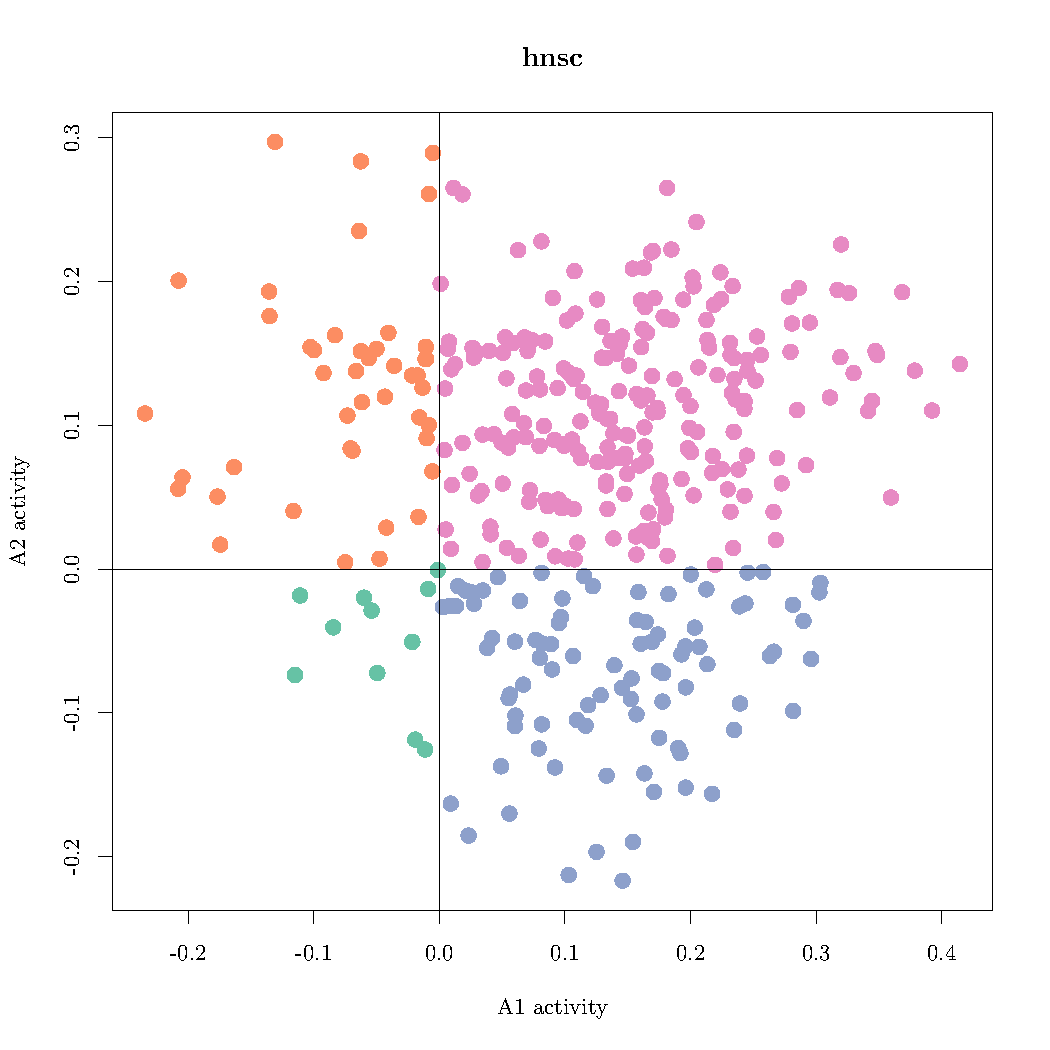
\includegraphics[width=\maxwidth]{figure/km-curves-7} 

}




{\centering 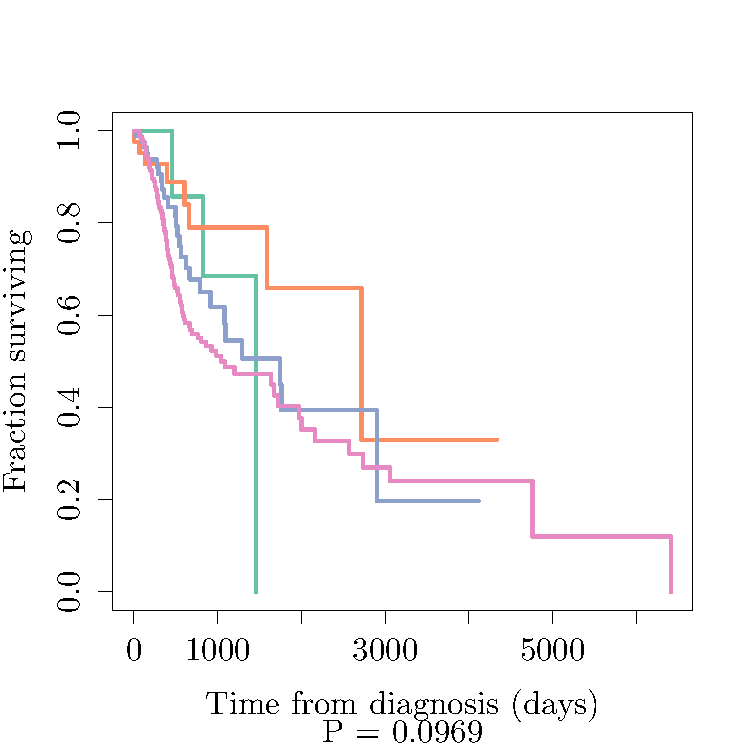
\includegraphics[width=\maxwidth]{figure/km-curves-8} 

}


\begin{kframe}\begin{alltt}
\hlkwd{plot_km_axes_tcga}\hlstd{(}\hlstr{"kirc"}\hlstd{,} \hlkwc{mc} \hlstd{=} \hlnum{FALSE}\hlstd{)}
\end{alltt}
\begin{verbatim}
## Call: survfit(formula = y ~ class)
## 
##          records n.max n.start events median 0.95LCL 0.95UCL
## class=LL      77    77      77     17   2763    2385      NA
## class=LH     179   179     179     42   2600    2343      NA
## class=HL      96    96      96     25   2830    2190      NA
## class=HH     146   146     146     69   1432    1200    1964
## Call:
## survdiff(formula = y ~ class)
## 
##            N Observed Expected (O-E)^2/E (O-E)^2/V
## class=LL  77       17     26.8      3.59      4.39
## class=LH 179       42     55.3      3.21      5.08
## class=HL  96       25     32.0      1.54      1.96
## class=HH 146       69     38.8     23.44     31.71
## 
##  Chisq= 32.1  on 3 degrees of freedom, p= 5e-07
\end{verbatim}
\end{kframe}

{\centering 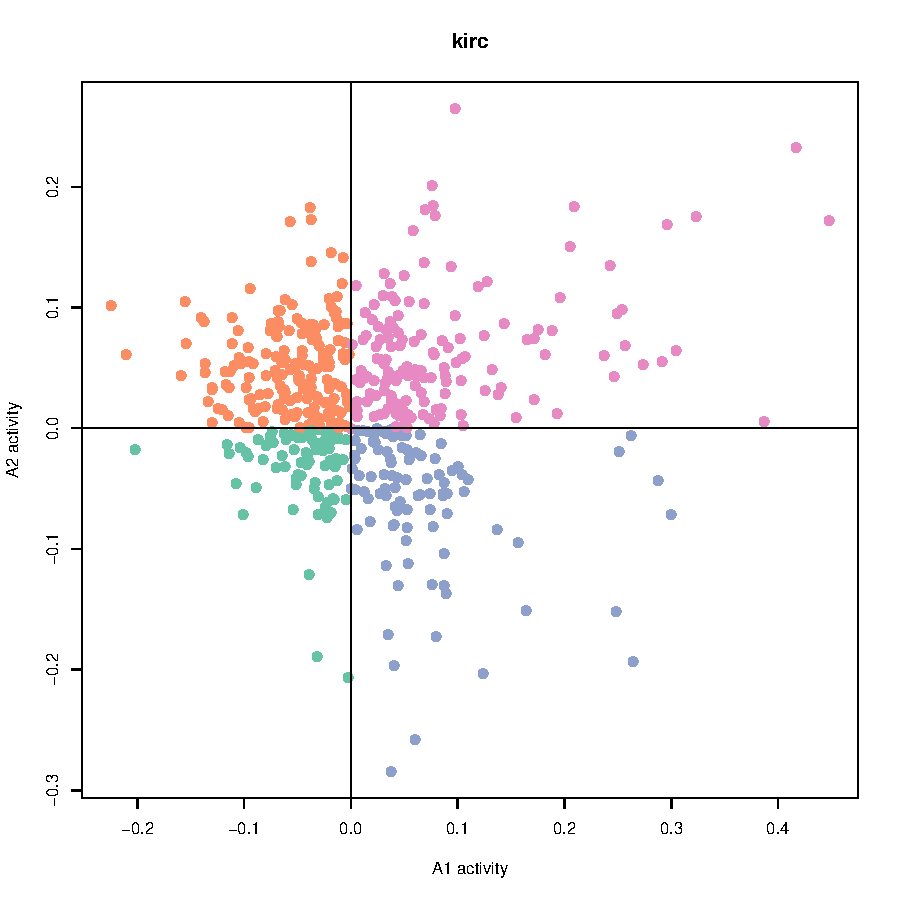
\includegraphics[width=\maxwidth]{figure/km-curves-9} 

}




{\centering 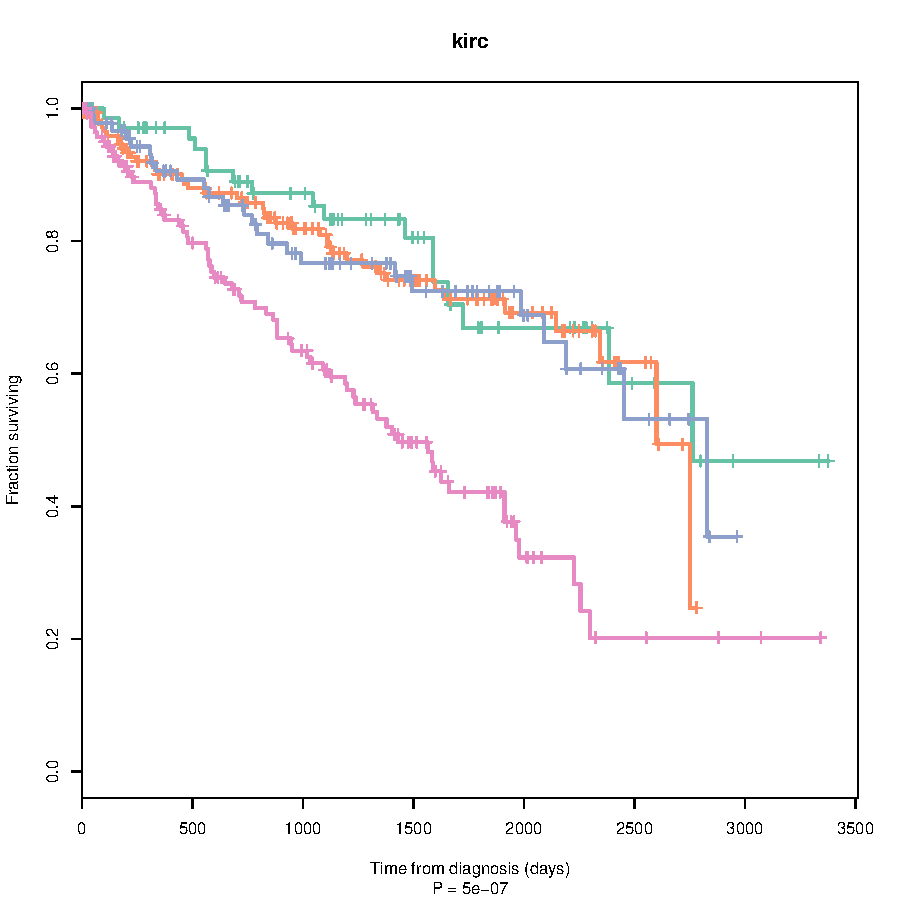
\includegraphics[width=\maxwidth]{figure/km-curves-10} 

}


\begin{kframe}\begin{alltt}
\hlkwd{plot_km_axes_tcga}\hlstd{(}\hlstr{"lgg"}\hlstd{,} \hlkwc{mc} \hlstd{=} \hlnum{FALSE}\hlstd{)}
\end{alltt}


{\ttfamily\noindent\color{warningcolor}{\#\# Warning in plot\_km\_axes\_tcga("{}lgg"{}, mc = FALSE): NAs introduced by coercion}}\begin{verbatim}
## Call: survfit(formula = y ~ class)
## 
##          records n.max n.start events median 0.95LCL 0.95UCL
## class=LL      77    77      77      4     NA    1762      NA
## class=LH      32    32      32      3   2907    2660      NA
## class=HL     106   106     106     28   2051    1886    3978
## class=HH      57    57      57     18   1915     682      NA
## Call:
## survdiff(formula = y ~ class)
## 
##            N Observed Expected (O-E)^2/E (O-E)^2/V
## class=LL  77        4     9.86     3.479     4.389
## class=LH  32        3     5.38     1.055     1.191
## class=HL 106       28    26.36     0.102     0.207
## class=HH  57       18    11.40     3.815     4.950
## 
##  Chisq= 8.7  on 3 degrees of freedom, p= 0.0333
\end{verbatim}
\end{kframe}

{\centering 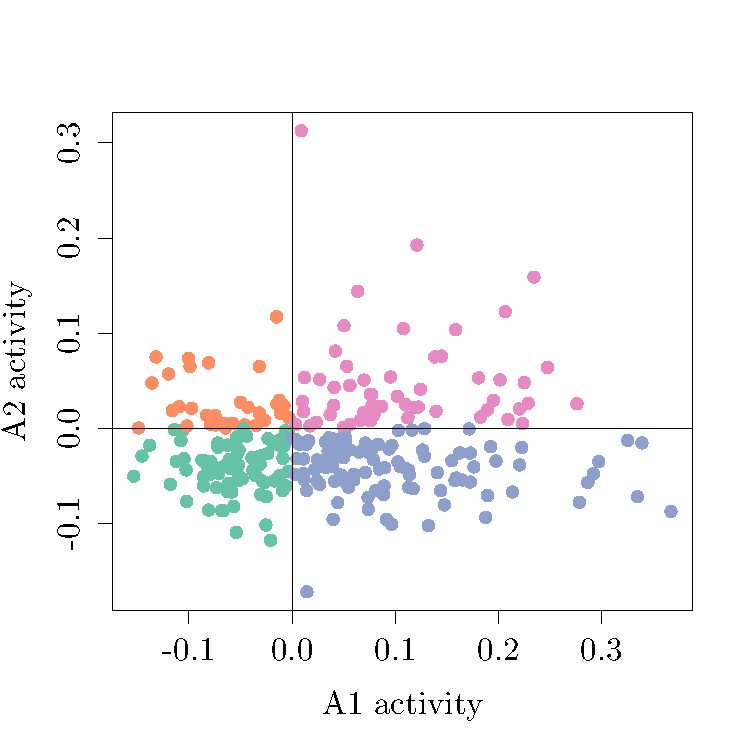
\includegraphics[width=\maxwidth]{figure/km-curves-11} 

}




{\centering 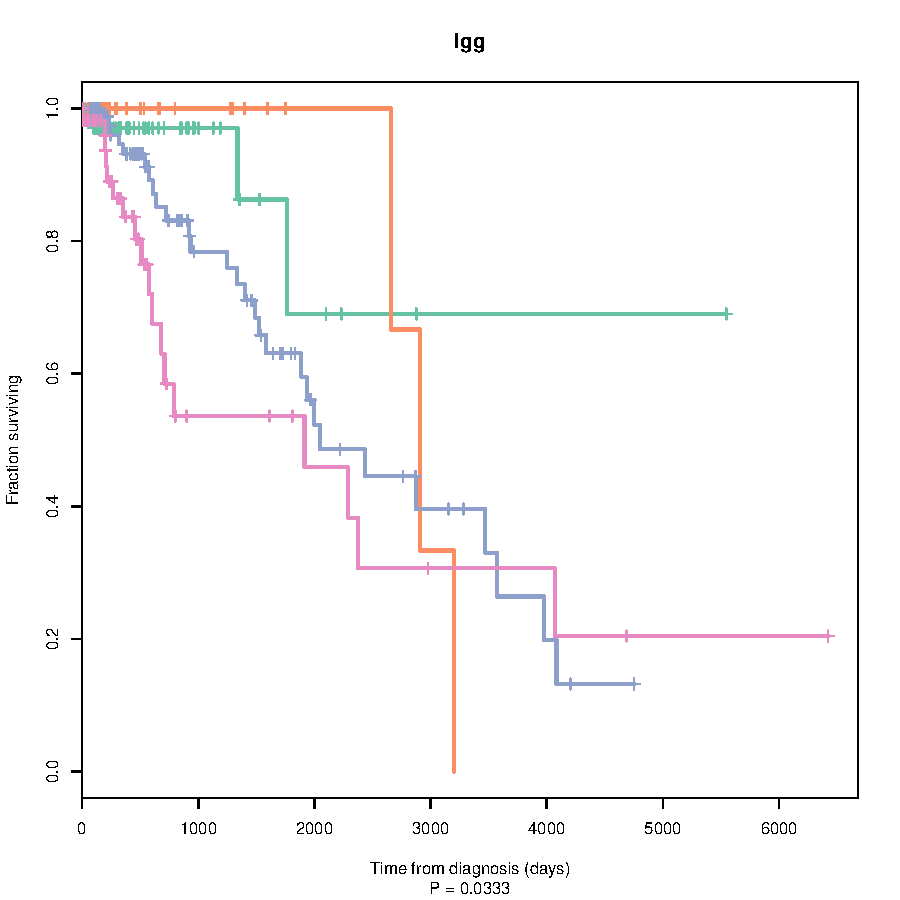
\includegraphics[width=\maxwidth]{figure/km-curves-12} 

}


\begin{kframe}\begin{alltt}
\hlkwd{plot_km_axes_tcga}\hlstd{(}\hlstr{"luad"}\hlstd{,} \hlkwc{mc} \hlstd{=} \hlnum{FALSE}\hlstd{)}
\end{alltt}


{\ttfamily\noindent\color{warningcolor}{\#\# Warning in plot\_km\_axes\_tcga("{}luad"{}, mc = FALSE): NAs introduced by coercion}}\begin{verbatim}
## Call: survfit(formula = y ~ class)
## 
##    19 observations deleted due to missingness 
##          records n.max n.start events median 0.95LCL 0.95UCL
## class=LL     102   102     102     18   1790    1421      NA
## class=LH      49    49      49      9   1599    1147      NA
## class=HL      98    98      98     26   1491     807      NA
## class=HH     182   182     182     53   1042     863    1379
## Call:
## survdiff(formula = y ~ class)
## 
## n=431, 19 observations deleted due to missingness.
## 
##            N Observed Expected (O-E)^2/E (O-E)^2/V
## class=LL 102       18     28.0    3.5523     4.875
## class=LH  49        9     11.9    0.6911     0.786
## class=HL  98       26     27.5    0.0801     0.112
## class=HH 182       53     38.7    5.2967     8.567
## 
##  Chisq= 9.8  on 3 degrees of freedom, p= 0.0203
\end{verbatim}
\end{kframe}

{\centering 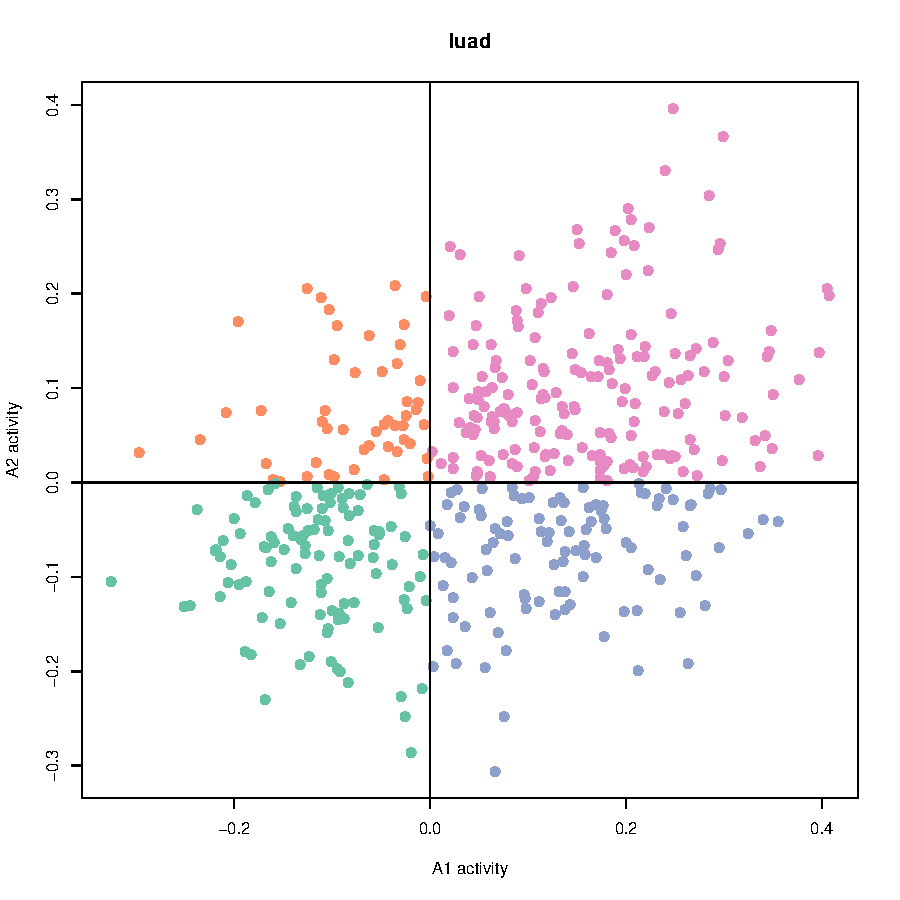
\includegraphics[width=\maxwidth]{figure/km-curves-13} 

}




{\centering 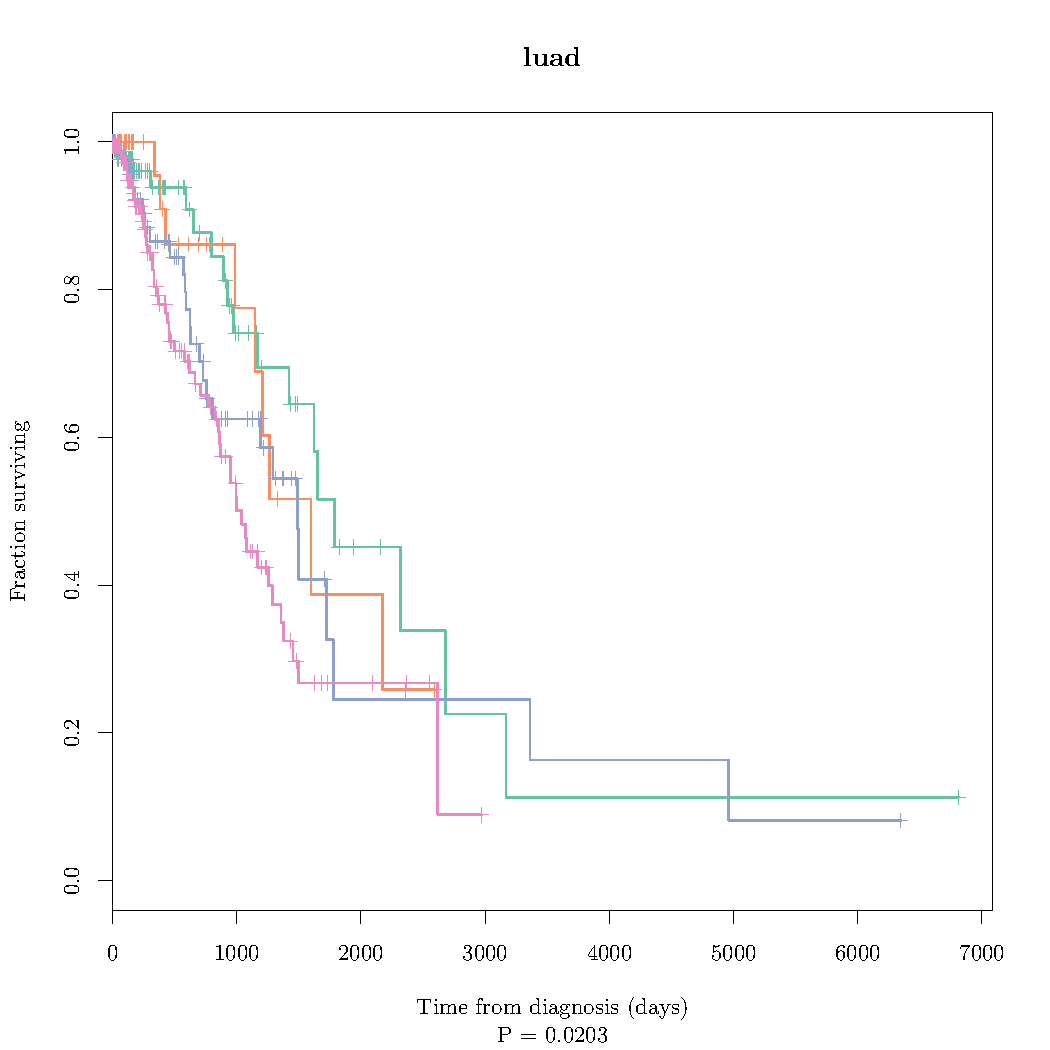
\includegraphics[width=\maxwidth]{figure/km-curves-14} 

}


\begin{kframe}\begin{alltt}
\hlkwd{plot_km_axes_tcga}\hlstd{(}\hlstr{"paad"}\hlstd{,} \hlkwc{mc} \hlstd{=} \hlnum{FALSE}\hlstd{)}
\end{alltt}
\begin{verbatim}
## Call: survfit(formula = y ~ class)
## 
##          records n.max n.start events median 0.95LCL 0.95UCL
## class=LL       9     9       9      2    906     480      NA
## class=LH      19    19      19      4    485     467      NA
## class=HL       9     9       9      2    665     334      NA
## class=HH      21    21      21      9    460     145      NA
## Call:
## survdiff(formula = y ~ class)
## 
##           N Observed Expected (O-E)^2/E (O-E)^2/V
## class=LL  9        2     3.13     0.408     0.536
## class=LH 19        4     5.86     0.592     1.052
## class=HL  9        2     2.71     0.187     0.233
## class=HH 21        9     5.29     2.593     4.105
## 
##  Chisq= 4.2  on 3 degrees of freedom, p= 0.244
\end{verbatim}
\end{kframe}

{\centering 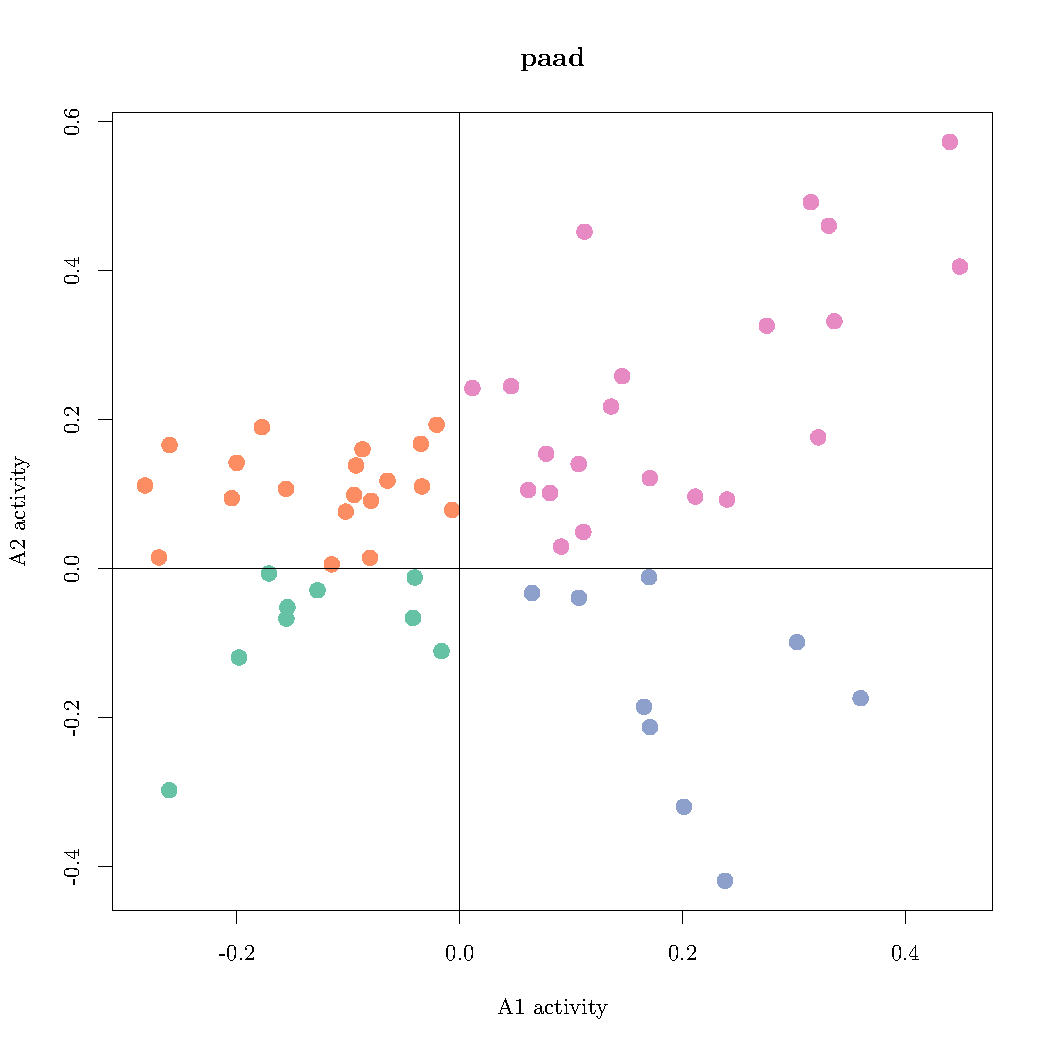
\includegraphics[width=\maxwidth]{figure/km-curves-15} 

}




{\centering 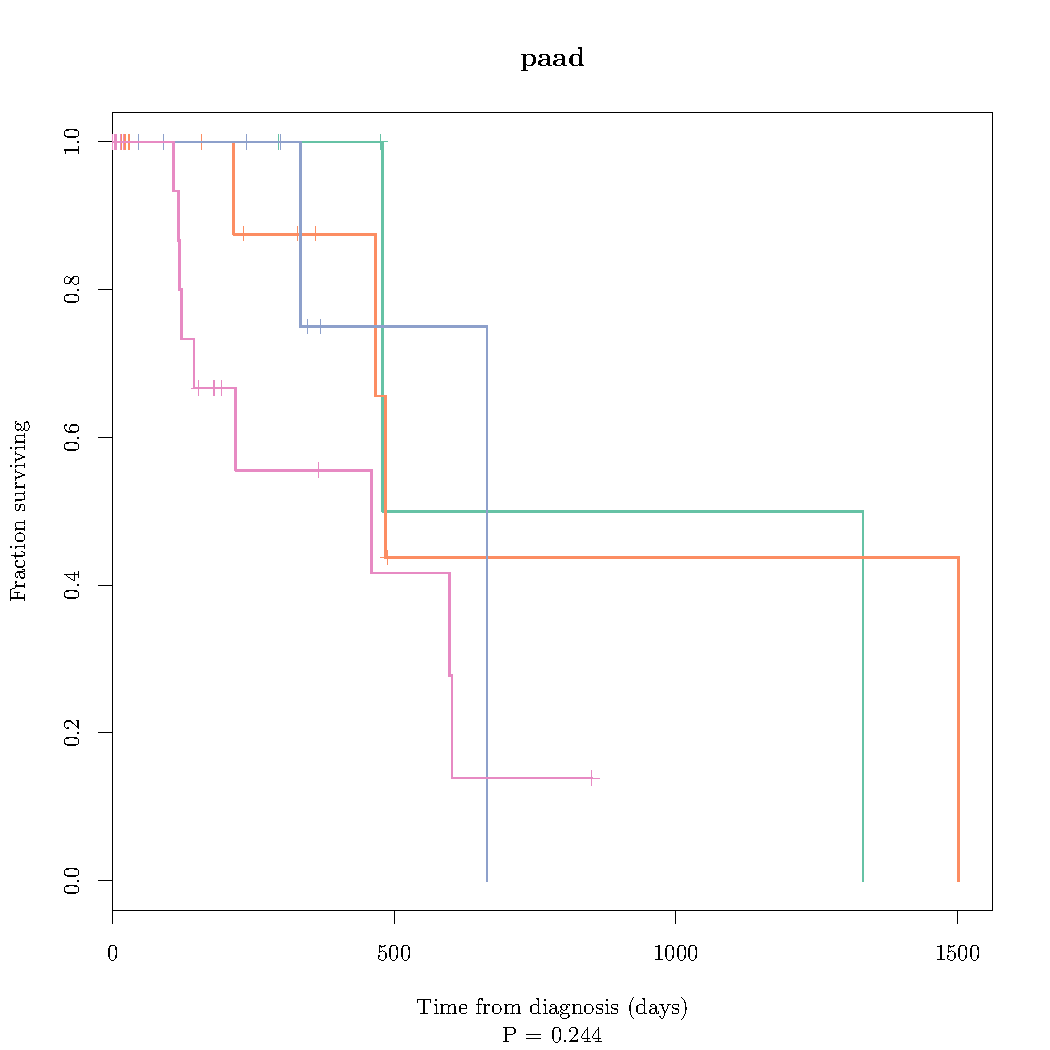
\includegraphics[width=\maxwidth]{figure/km-curves-16} 

}



\end{knitrout}


%%%%%%%%%%%%%%%%%%%%%%%%%%%%%%%%%%%%%%%%%%%%%%%%%%%%%%%%%%%%%%%%%%%%%%
% SIGNATURE BIOLOGY
%%%%%%%%%%%%%%%%%%%%%%%%%%%%%%%%%%%%%%%%%%%%%%%%%%%%%%%%%%%%%%%%%%%%%%
\subsection{MSigDB score correlation thresholding}
\begin{knitrout}
\definecolor{shadecolor}{rgb}{0.969, 0.969, 0.969}\color{fgcolor}\begin{kframe}
\begin{alltt}
\hlstd{axis_coefs.msigdb.corr} \hlkwb{=} \hlkwd{cor}\hlstd{(axis_coefs.diag_dsd,} \hlkwd{t}\hlstd{(sigs),} \hlkwc{method} \hlstd{=} \hlstr{"kendall"}\hlstd{)}

\hlstd{temp.sel_cols} \hlkwb{=} \hlkwd{apply}\hlstd{(}\hlkwd{abs}\hlstd{(axis_coefs.msigdb.corr)} \hlopt{>=} \hlstd{sig.corr.threshold,} \hlnum{2}\hlstd{,}
    \hlstd{any)}
\hlkwd{heatmap.2}\hlstd{(axis_coefs.msigdb.corr[, temp.sel_cols],} \hlkwc{trace} \hlstd{=} \hlstr{"none"}\hlstd{,} \hlkwc{scale} \hlstd{=} \hlstr{"none"}\hlstd{,}
    \hlkwc{useRaster} \hlstd{=} \hlnum{TRUE}\hlstd{,} \hlkwc{col} \hlstd{=} \hlkwd{brewer.pal}\hlstd{(}\hlnum{11}\hlstd{,} \hlstr{"PiYG"}\hlstd{),} \hlkwc{symbreaks} \hlstd{=} \hlnum{TRUE}\hlstd{)}
\end{alltt}
\end{kframe}

{\centering 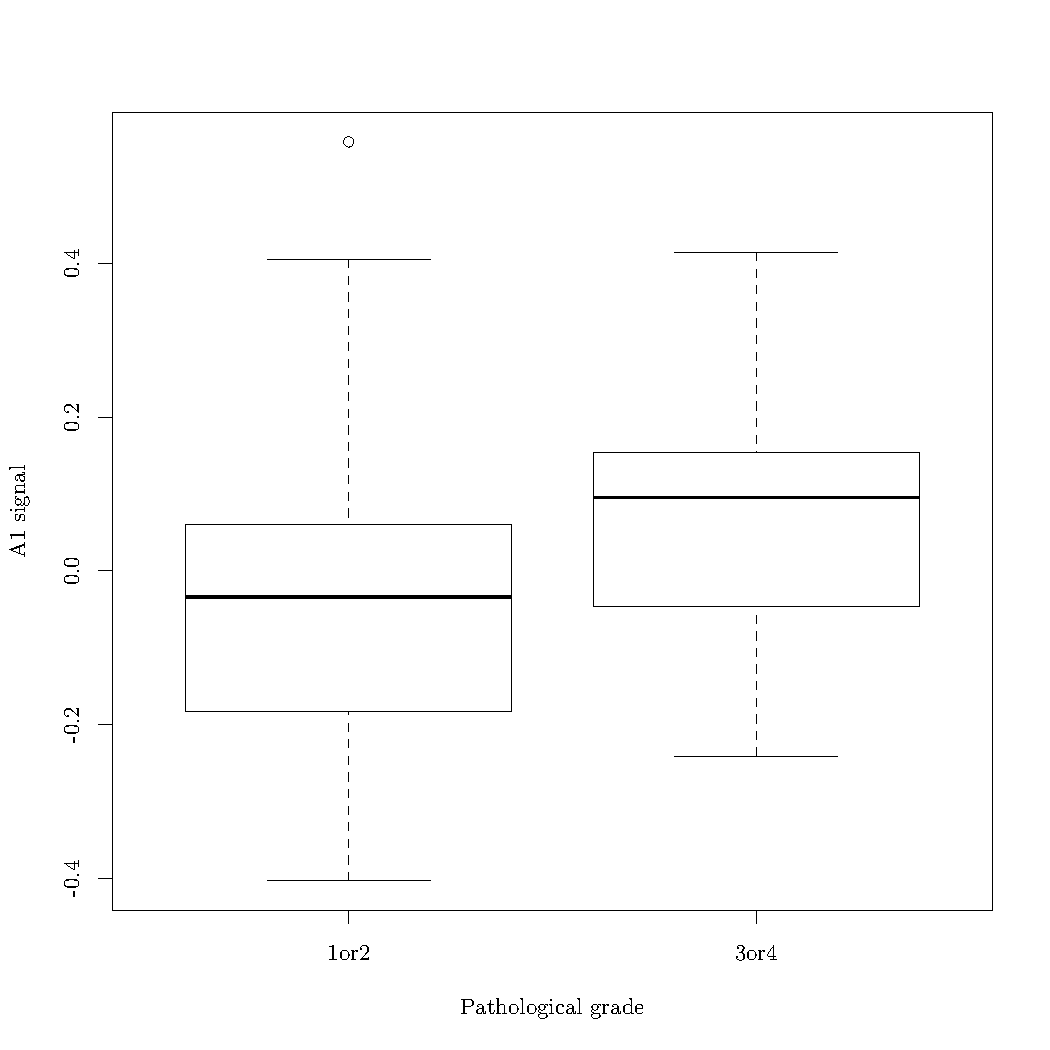
\includegraphics[width=\maxwidth]{figure/nmf-msigdb-cor-plots-1} 

}


\begin{kframe}\begin{alltt}
\hlkwd{heatmap.2}\hlstd{(axis_coefs.msigdb.corr[, temp.sel_cols],} \hlkwc{trace} \hlstd{=} \hlstr{"none"}\hlstd{,} \hlkwc{scale} \hlstd{=} \hlstr{"none"}\hlstd{,}
    \hlkwc{useRaster} \hlstd{=} \hlnum{TRUE}\hlstd{,} \hlkwc{col} \hlstd{=} \hlkwd{brewer.pal}\hlstd{(}\hlnum{3}\hlstd{,} \hlstr{"PiYG"}\hlstd{),} \hlkwc{breaks} \hlstd{=} \hlkwd{c}\hlstd{(}\hlopt{-}\hlnum{1}\hlstd{,} \hlopt{-}\hlstd{sig.corr.threshold,}
        \hlstd{sig.corr.threshold,} \hlnum{1}\hlstd{))}
\end{alltt}
\end{kframe}

{\centering 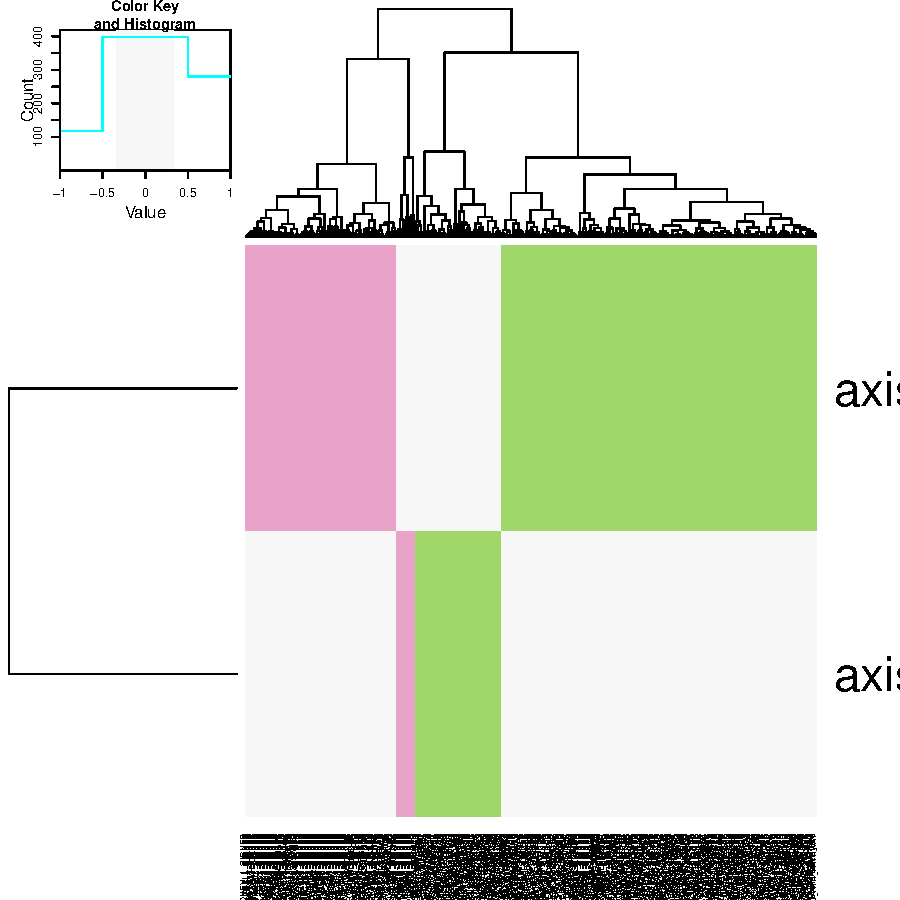
\includegraphics[width=\maxwidth]{figure/nmf-msigdb-cor-plots-2} 

}


\begin{kframe}\begin{alltt}
\hlstd{cpv.pvals} \hlkwb{=} \hlkwd{apply}\hlstd{(axis_coefs.diag_dsd,} \hlnum{2}\hlstd{,} \hlkwa{function}\hlstd{(}\hlkwc{mg}\hlstd{)} \hlkwd{sapply}\hlstd{(}\hlkwd{cbind}\hlstd{(cpvs.diag_dsd,}
    \hlkwc{purity} \hlstd{= samps.diag_dsd}\hlopt{$}\hlstd{purity_qpure),} \hlkwa{function}\hlstd{(}\hlkwc{x}\hlstd{) \{}
    \hlstd{s} \hlkwb{=} \hlopt{!}\hlkwd{is.na}\hlstd{(mg)} \hlopt{& !}\hlkwd{is.na}\hlstd{(x)}
    \hlstd{x} \hlkwb{=} \hlstd{x[s]}
    \hlstd{mg} \hlkwb{=} \hlstd{mg[s]}
    \hlkwa{if} \hlstd{(}\hlkwd{any}\hlstd{(}\hlkwd{c}\hlstd{(}\hlstr{"numeric"}\hlstd{,} \hlstr{"integer"}\hlstd{)} \hlopt \hlkwd{class}\hlstd{(x))) \{}
        \hlkwd{return}\hlstd{(}\hlkwd{cor.test}\hlstd{(x, mg,} \hlkwc{method} \hlstd{=} \hlstr{"pearson"}\hlstd{)}\hlopt{$}\hlstd{p.value)}
    \hlstd{\}} \hlkwa{else if} \hlstd{(}\hlkwd{any}\hlstd{(}\hlkwd{c}\hlstd{(}\hlstr{"factor"}\hlstd{,} \hlstr{"ordered"}\hlstd{,} \hlstr{"logical"}\hlstd{)} \hlopt \hlkwd{class}\hlstd{(x))} \hlopt{&&} \hlkwd{length}\hlstd{(}\hlkwd{unique}\hlstd{(x))} \hlopt{>}
        \hlnum{1}\hlstd{) \{}
        \hlkwd{return}\hlstd{(}\hlkwd{anova}\hlstd{(}\hlkwd{lm}\hlstd{(mg} \hlopt{~} \hlstd{x))[,} \hlstr{"Pr(>F)"}\hlstd{][}\hlnum{1}\hlstd{])}
    \hlstd{\}}
    \hlnum{NA}
\hlstd{\}))}
\hlstd{cpv.pvals} \hlkwb{=} \hlstd{cpv.pvals[}\hlopt{!}\hlkwd{apply}\hlstd{(}\hlkwd{is.na}\hlstd{(cpv.pvals),} \hlnum{1}\hlstd{, all), ]}
\hlstd{cpv.pvals} \hlkwb{=} \hlstd{cpv.pvals[}\hlopt{!}\hlkwd{grepl}\hlstd{(}\hlstr{"^Surv\textbackslash{}\textbackslash{}."}\hlstd{,} \hlkwd{rownames}\hlstd{(cpv.pvals)), ]}
\hlstd{cpv.pvals} \hlkwb{=} \hlstd{cpv.pvals[}\hlopt{!}\hlkwd{grepl}\hlstd{(}\hlstr{"^Treat\textbackslash{}\textbackslash{}."}\hlstd{,} \hlkwd{rownames}\hlstd{(cpv.pvals)), ]}
\hlstd{cpv.pvals} \hlkwb{=} \hlstd{cpv.pvals[}\hlopt{!}\hlkwd{grepl}\hlstd{(}\hlstr{"^Path\textbackslash{}\textbackslash{}.Nodes"}\hlstd{,} \hlkwd{rownames}\hlstd{(cpv.pvals)), ]}
\hlstd{cpv.pvals} \hlkwb{=} \hlstd{cpv.pvals[}\hlopt{!}\hlkwd{grepl}\hlstd{(}\hlstr{"^Staging\textbackslash{}\textbackslash{}.Version"}\hlstd{,} \hlkwd{rownames}\hlstd{(cpv.pvals)), ]}
\hlstd{cpv.pvals} \hlkwb{=} \hlstd{cpv.pvals[}\hlopt{!}\hlkwd{grepl}\hlstd{(}\hlstr{"^History\textbackslash{}\textbackslash{}.Recurrence$"}\hlstd{,} \hlkwd{rownames}\hlstd{(cpv.pvals)),}
    \hlstd{]}
\hlstd{cpv.pvals} \hlkwb{=} \hlstd{cpv.pvals[}\hlopt{!}\hlkwd{grepl}\hlstd{(}\hlstr{"^History\textbackslash{}\textbackslash{}.Status$"}\hlstd{,} \hlkwd{rownames}\hlstd{(cpv.pvals)), ]}
\hlstd{cpv.pvals} \hlkwb{=} \hlstd{cpv.pvals[}\hlopt{!}\hlkwd{grepl}\hlstd{(}\hlstr{"^History\textbackslash{}\textbackslash{}.Death\textbackslash{}\textbackslash{}.Cause$"}\hlstd{,} \hlkwd{rownames}\hlstd{(cpv.pvals)),}
    \hlstd{]}
\hlstd{cpv.pvals} \hlkwb{=} \hlstd{cpv.pvals[}\hlopt{!}\hlkwd{grepl}\hlstd{(}\hlstr{"^Path\textbackslash{}\textbackslash{}.Grade$"}\hlstd{,} \hlkwd{rownames}\hlstd{(cpv.pvals)), ]}
\hlstd{cpv.pvals} \hlkwb{=} \hlstd{cpv.pvals[}\hlopt{!}\hlkwd{grepl}\hlstd{(}\hlstr{"^Path\textbackslash{}\textbackslash{}.TumourLocation$"}\hlstd{,} \hlkwd{rownames}\hlstd{(cpv.pvals)),}
    \hlstd{]}

\hlstd{temp} \hlkwb{=} \hlkwd{as.vector}\hlstd{(cpv.pvals)}
\hlstd{temp} \hlkwb{=} \hlkwd{p.adjust}\hlstd{(temp,} \hlstr{"holm"}\hlstd{)}
\hlstd{cpv.qvals} \hlkwb{=} \hlkwd{matrix}\hlstd{(temp,} \hlkwc{nrow} \hlstd{=} \hlkwd{nrow}\hlstd{(cpv.pvals))}
\hlkwd{rownames}\hlstd{(cpv.qvals)} \hlkwb{=} \hlkwd{rownames}\hlstd{(cpv.pvals)}
\hlkwd{colnames}\hlstd{(cpv.qvals)} \hlkwb{=} \hlkwd{colnames}\hlstd{(cpv.pvals)}

\hlstd{cpv.pvals}
\end{alltt}
\begin{verbatim}
##                                         axis1     axis2
## Patient.Gender                      0.1581541 0.0098535
## Patient.Ethnicity                   0.7711156 0.1130046
## History.Smoking.PackYears           0.3562152 0.2753851
## History.Diagnosis.AgeAtYears        0.9250804 0.6658699
## Path.HistoType.Subtype              0.6966533 0.1569139
## Path.TumourSizeMm                   0.8438715 0.1709600
## Path.Invasion.PN                    0.0951996 0.2251091
## Path.Invasion.VS                    0.6500594 0.0707968
## Staging.pM                          0.4414498 0.4245233
## Staging.pN                          0.2524195 0.2629997
## Staging.pT                          0.2640385 0.4273685
## Staging.Stage                       0.0605854 0.2355348
## History.Recurrence.Site.Peritoneum  0.9162045 0.0149891
## History.Recurrence.Site.PancRemnant 0.5341395 0.1839586
## History.Recurrence.Site.PancBed     0.8869735 0.5303110
## History.Recurrence.Site.Other       0.1930828 0.1614602
## History.Recurrence.Site.Omentum     0.1388378 0.0820434
## History.Recurrence.Site.Mesentery   0.9326763 0.1206991
## History.Recurrence.Site.LymphNodes  0.9332622 0.8703023
## History.Recurrence.Site.Lung        0.3900712 0.7130517
## History.Recurrence.Site.Liver       0.1596616 0.1046158
## History.Recurrence.Site.Brain       0.4296978 0.0621650
## History.Recurrence.Site.Bone        0.7889803 0.4128670
## Path.Grade.Coarse                   0.0023854 0.0001297
## Path.TumourLocation.Coarse          0.1767526 0.1392750
## purity                              0.0002129 0.0004113
\end{verbatim}
\begin{alltt}
\hlstd{cpv.qvals}
\end{alltt}
\begin{verbatim}
##                                       axis1    axis2
## Patient.Gender                      1.00000 0.472968
## Patient.Ethnicity                   1.00000 1.000000
## History.Smoking.PackYears           1.00000 1.000000
## History.Diagnosis.AgeAtYears        1.00000 1.000000
## Path.HistoType.Subtype              1.00000 1.000000
## Path.TumourSizeMm                   1.00000 1.000000
## Path.Invasion.PN                    1.00000 1.000000
## Path.Invasion.VS                    1.00000 1.000000
## Staging.pM                          1.00000 1.000000
## Staging.pN                          1.00000 1.000000
## Staging.pT                          1.00000 1.000000
## Staging.Stage                       1.00000 1.000000
## History.Recurrence.Site.Peritoneum  1.00000 0.704486
## History.Recurrence.Site.PancRemnant 1.00000 1.000000
## History.Recurrence.Site.PancBed     1.00000 1.000000
## History.Recurrence.Site.Other       1.00000 1.000000
## History.Recurrence.Site.Omentum     1.00000 1.000000
## History.Recurrence.Site.Mesentery   1.00000 1.000000
## History.Recurrence.Site.LymphNodes  1.00000 1.000000
## History.Recurrence.Site.Lung        1.00000 1.000000
## History.Recurrence.Site.Liver       1.00000 1.000000
## History.Recurrence.Site.Brain       1.00000 1.000000
## History.Recurrence.Site.Bone        1.00000 1.000000
## Path.Grade.Coarse                   0.11688 0.006743
## Path.TumourLocation.Coarse          1.00000 1.000000
## purity                              0.01086 0.020564
\end{verbatim}
\begin{alltt}
\hlkwd{boxplot}\hlstd{(axis_coefs.diag_dsd[,} \hlnum{1}\hlstd{]} \hlopt{~} \hlstd{cpvs.diag_dsd}\hlopt{$}\hlstd{Path.Grade.Coarse,} \hlkwc{xlab} \hlstd{=} \hlstr{"Pathological grade"}\hlstd{,}
    \hlkwc{ylab} \hlstd{=} \hlstr{"A1 signal"}\hlstd{)}
\end{alltt}
\end{kframe}

{\centering 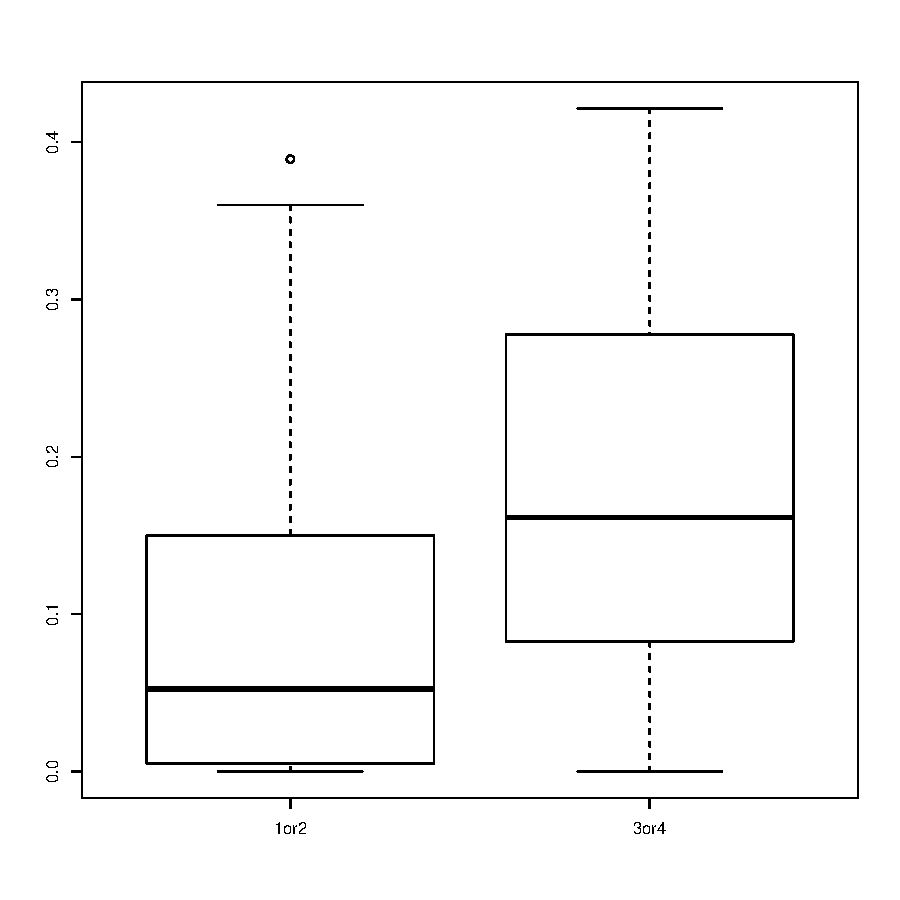
\includegraphics[width=\maxwidth]{figure/nmf-msigdb-cor-plots-3} 

}


\begin{kframe}\begin{alltt}
\hlkwd{boxplot}\hlstd{(axis_coefs.diag_dsd[,} \hlnum{2}\hlstd{]} \hlopt{~} \hlstd{cpvs.diag_dsd}\hlopt{$}\hlstd{Path.Grade.Coarse,} \hlkwc{xlab} \hlstd{=} \hlstr{"Pathological grade"}\hlstd{,}
    \hlkwc{ylab} \hlstd{=} \hlstr{"A2 signal"}\hlstd{)}
\end{alltt}
\end{kframe}

{\centering 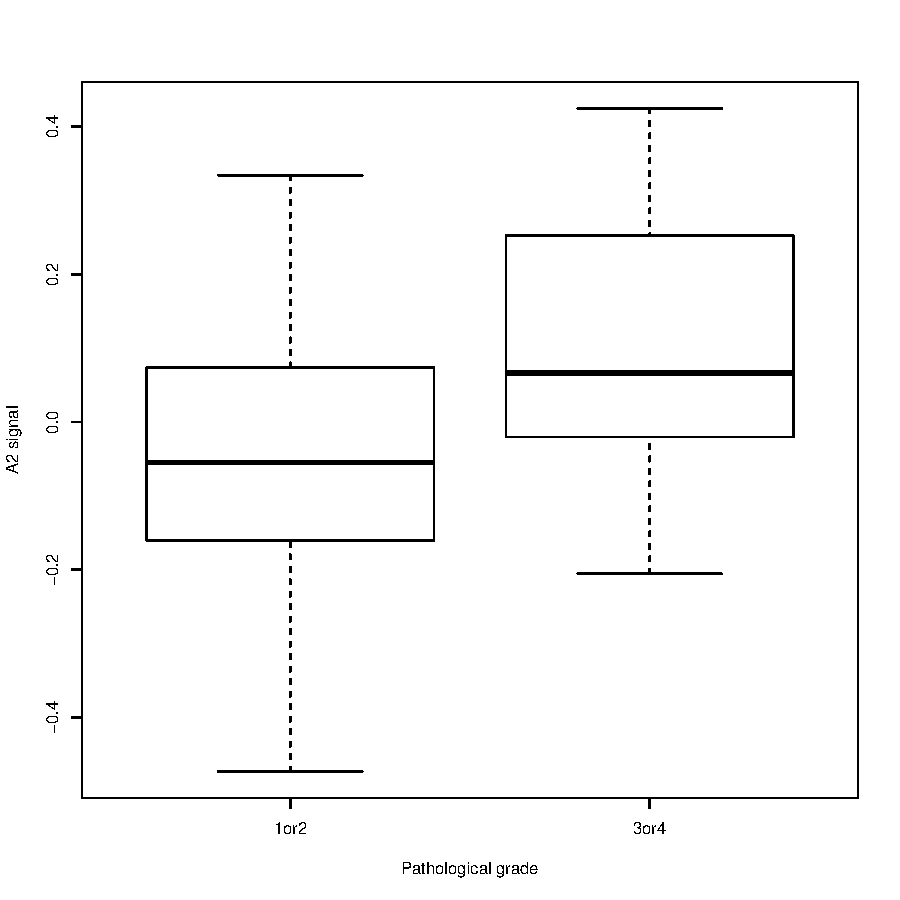
\includegraphics[width=\maxwidth]{figure/nmf-msigdb-cor-plots-4} 

}


\begin{kframe}\begin{alltt}
\hlkwd{lm}\hlstd{(axis_coefs.diag_dsd[,} \hlnum{2}\hlstd{]} \hlopt{~} \hlstd{cpvs.diag_dsd}\hlopt{$}\hlstd{Path.Grade.Coarse)}
\end{alltt}
\begin{verbatim}
## 
## Call:
## lm(formula = axis_coefs.diag_dsd[, 2] ~ cpvs.diag_dsd$Path.Grade.Coarse)
## 
## Coefficients:
##                       (Intercept)  cpvs.diag_dsd$Path.Grade.Coarse.L  
##                            0.0261                             0.1103
\end{verbatim}
\begin{alltt}
\hlkwd{summary}\hlstd{(}\hlkwd{lm}\hlstd{(axis_coefs.diag_dsd[,} \hlnum{2}\hlstd{]} \hlopt{~} \hlstd{cpvs.diag_dsd}\hlopt{$}\hlstd{Path.Grade.Coarse))}
\end{alltt}
\begin{verbatim}
## 
## Call:
## lm(formula = axis_coefs.diag_dsd[, 2] ~ cpvs.diag_dsd$Path.Grade.Coarse)
## 
## Residuals:
##     Min      1Q  Median      3Q     Max 
## -0.4212 -0.1130 -0.0137  0.1372  0.3860 
## 
## Coefficients:
##                                   Estimate Std. Error t value Pr(>|t|)
## (Intercept)                         0.0261     0.0197    1.33  0.18771
## cpvs.diag_dsd$Path.Grade.Coarse.L   0.1103     0.0278    3.97  0.00013
## 
## Residual standard error: 0.185 on 108 degrees of freedom
## Multiple R-squared:  0.127,	Adjusted R-squared:  0.119 
## F-statistic: 15.8 on 1 and 108 DF,  p-value: 0.00013
\end{verbatim}
\begin{alltt}
\hlkwd{anova}\hlstd{(}\hlkwd{lm}\hlstd{(axis_coefs.diag_dsd[,} \hlnum{2}\hlstd{]} \hlopt{~} \hlstd{cpvs.diag_dsd}\hlopt{$}\hlstd{Path.Grade.Coarse))}
\end{alltt}
\begin{verbatim}
## Analysis of Variance Table
## 
## Response: axis_coefs.diag_dsd[, 2]
##                                  Df Sum Sq Mean Sq F value  Pr(>F)
## cpvs.diag_dsd$Path.Grade.Coarse   1   0.54   0.542    15.8 0.00013
## Residuals                       108   3.71   0.034
\end{verbatim}
\begin{alltt}
\hlkwd{plot}\hlstd{(axis_coefs.diag_dsd[,} \hlnum{1}\hlstd{]} \hlopt{~} \hlstd{samps}\hlopt{$}\hlstd{purity_qpure,} \hlkwc{xlab} \hlstd{=} \hlstr{"qPure estimate"}\hlstd{,}
    \hlkwc{ylab} \hlstd{=} \hlstr{"A1 signal"}\hlstd{)}
\end{alltt}
\end{kframe}

{\centering 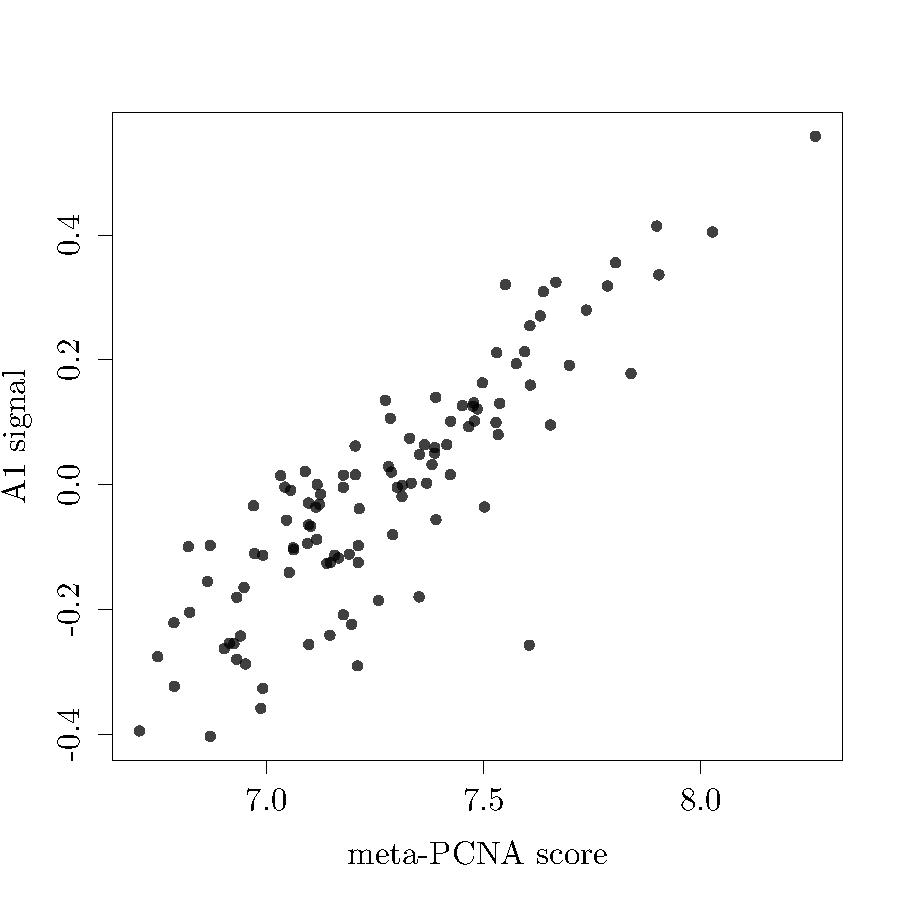
\includegraphics[width=\maxwidth]{figure/nmf-msigdb-cor-plots-5} 

}


\begin{kframe}\begin{alltt}
\hlkwd{plot}\hlstd{(axis_coefs.diag_dsd[,} \hlnum{2}\hlstd{]} \hlopt{~} \hlstd{samps}\hlopt{$}\hlstd{purity_qpure,} \hlkwc{xlab} \hlstd{=} \hlstr{"qPure estimate"}\hlstd{,}
    \hlkwc{ylab} \hlstd{=} \hlstr{"A2 signal"}\hlstd{)}
\end{alltt}
\end{kframe}

{\centering 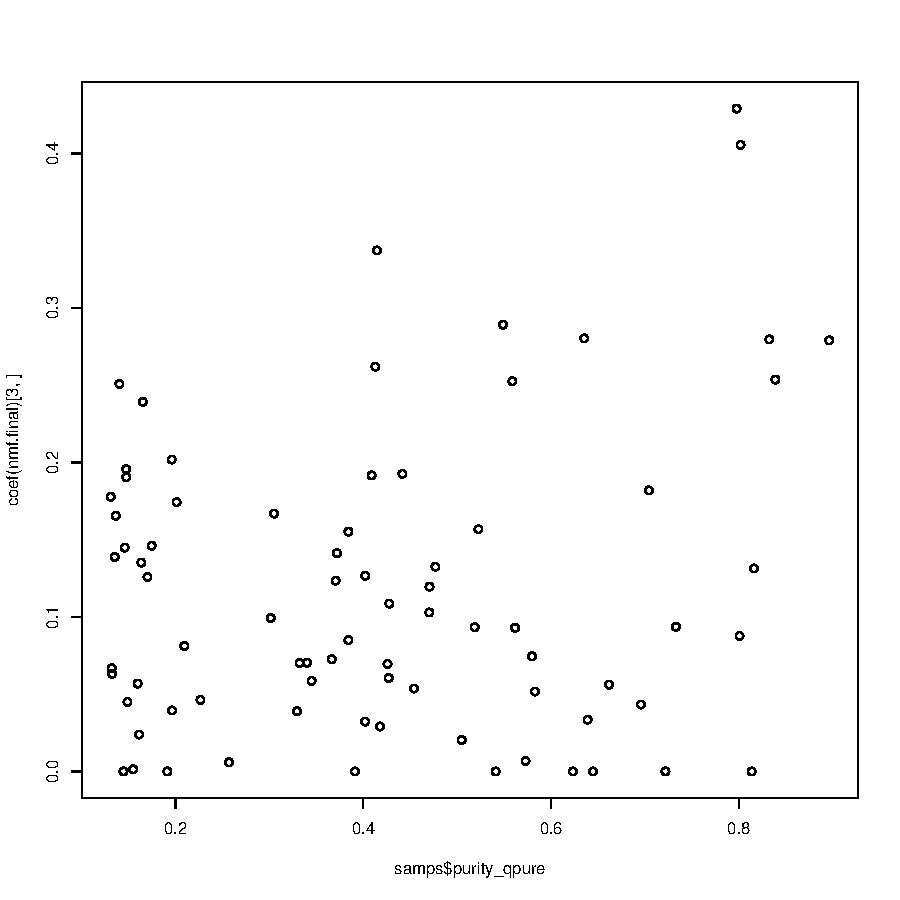
\includegraphics[width=\maxwidth]{figure/nmf-msigdb-cor-plots-6} 

}


\begin{kframe}\begin{alltt}
\hlkwd{cor.test}\hlstd{(axis_coefs.diag_dsd[,} \hlnum{1}\hlstd{], samps}\hlopt{$}\hlstd{purity_qpure,} \hlkwc{method} \hlstd{=} \hlstr{"kendall"}\hlstd{)}
\end{alltt}
\begin{verbatim}
## 
## 	Kendall's rank correlation tau
## 
## data:  axis_coefs.diag_dsd[, 1] and samps$purity_qpure
## z = 3.676, p-value = 0.0002369
## alternative hypothesis: true tau is not equal to 0
## sample estimates:
##    tau 
## 0.2838
\end{verbatim}
\begin{alltt}
\hlkwd{cor.test}\hlstd{(axis_coefs.diag_dsd[,} \hlnum{2}\hlstd{], samps}\hlopt{$}\hlstd{purity_qpure,} \hlkwc{method} \hlstd{=} \hlstr{"kendall"}\hlstd{)}
\end{alltt}
\begin{verbatim}
## 
## 	Kendall's rank correlation tau
## 
## data:  axis_coefs.diag_dsd[, 2] and samps$purity_qpure
## z = -3.598, p-value = 0.0003203
## alternative hypothesis: true tau is not equal to 0
## sample estimates:
##     tau 
## -0.2778
\end{verbatim}
\begin{alltt}
\hlkwd{summary}\hlstd{(}\hlkwd{lm}\hlstd{(axis_coefs.diag_dsd[,} \hlnum{1}\hlstd{]} \hlopt{~} \hlstd{samps}\hlopt{$}\hlstd{purity_qpure))}
\end{alltt}
\begin{verbatim}
## 
## Call:
## lm(formula = axis_coefs.diag_dsd[, 1] ~ samps$purity_qpure)
## 
## Residuals:
##     Min      1Q  Median      3Q     Max 
## -0.3318 -0.1172 -0.0469  0.1011  0.5422 
## 
## Coefficients:
##                    Estimate Std. Error t value Pr(>|t|)
## (Intercept)          -0.132      0.042   -3.14  0.00240
## samps$purity_qpure    0.346      0.089    3.89  0.00021
## 
## Residual standard error: 0.173 on 76 degrees of freedom
##   (32 observations deleted due to missingness)
## Multiple R-squared:  0.166,	Adjusted R-squared:  0.155 
## F-statistic: 15.1 on 1 and 76 DF,  p-value: 0.000213
\end{verbatim}
\begin{alltt}
\hlkwd{summary}\hlstd{(}\hlkwd{lm}\hlstd{(axis_coefs.diag_dsd[,} \hlnum{2}\hlstd{]} \hlopt{~} \hlstd{samps}\hlopt{$}\hlstd{purity_qpure))}
\end{alltt}
\begin{verbatim}
## 
## Call:
## lm(formula = axis_coefs.diag_dsd[, 2] ~ samps$purity_qpure)
## 
## Residuals:
##     Min      1Q  Median      3Q     Max 
## -0.3541 -0.1356 -0.0213  0.1531  0.6002 
## 
## Coefficients:
##                    Estimate Std. Error t value Pr(>|t|)
## (Intercept)          0.1195     0.0473    2.53  0.01363
## samps$purity_qpure  -0.3701     0.1001   -3.70  0.00041
## 
## Residual standard error: 0.195 on 76 degrees of freedom
##   (32 observations deleted due to missingness)
## Multiple R-squared:  0.152,	Adjusted R-squared:  0.141 
## F-statistic: 13.7 on 1 and 76 DF,  p-value: 0.000411
\end{verbatim}
\begin{alltt}
\hlkwd{plot}\hlstd{(axis_coefs.diag_dsd[,} \hlnum{1}\hlstd{]} \hlopt{~} \hlstd{metapcna.scores,} \hlkwc{xlab} \hlstd{=} \hlstr{"meta-PCNA score"}\hlstd{,} \hlkwc{ylab} \hlstd{=} \hlstr{"A1 signal"}\hlstd{)}
\end{alltt}
\end{kframe}

{\centering 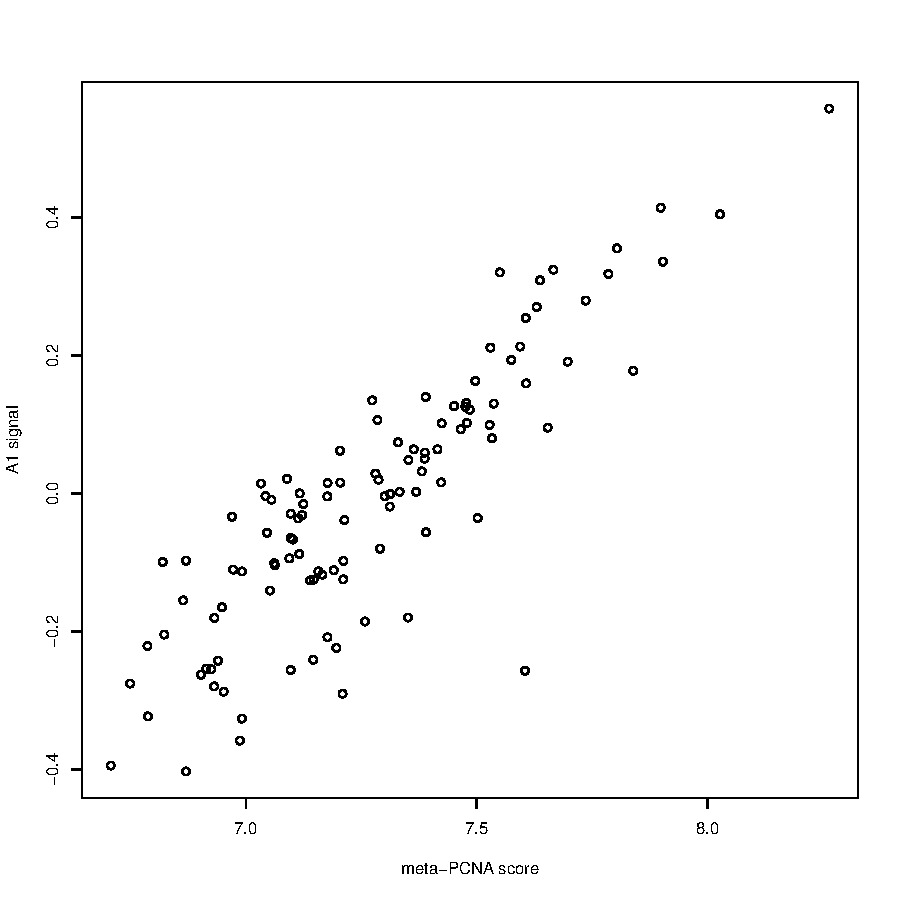
\includegraphics[width=\maxwidth]{figure/nmf-msigdb-cor-plots-7} 

}


\begin{kframe}\begin{alltt}
\hlkwd{plot}\hlstd{(axis_coefs.diag_dsd[,} \hlnum{2}\hlstd{]} \hlopt{~} \hlstd{metapcna.scores,} \hlkwc{xlab} \hlstd{=} \hlstr{"meta-PCNA score"}\hlstd{,} \hlkwc{ylab} \hlstd{=} \hlstr{"A2 signal"}\hlstd{)}
\end{alltt}
\end{kframe}

{\centering 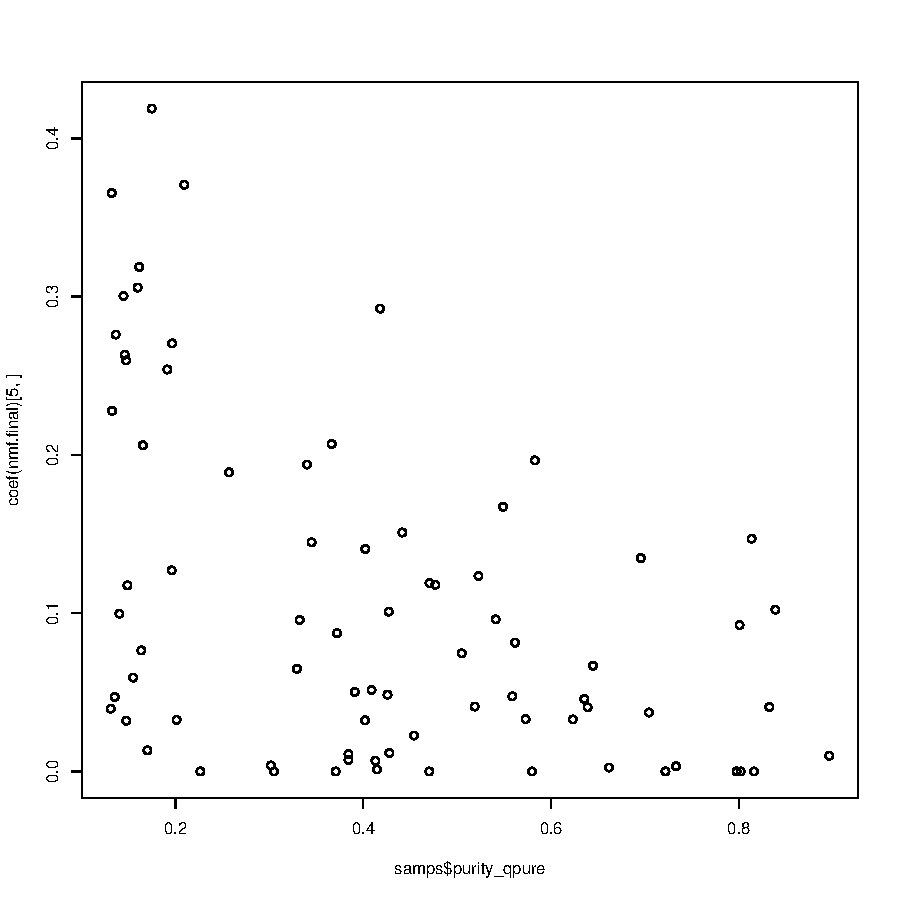
\includegraphics[width=\maxwidth]{figure/nmf-msigdb-cor-plots-8} 

}


\begin{kframe}\begin{alltt}
\hlkwd{cor.test}\hlstd{(axis_coefs.diag_dsd[,} \hlnum{1}\hlstd{], metapcna.scores,} \hlkwc{method} \hlstd{=} \hlstr{"kendall"}\hlstd{)}
\end{alltt}
\begin{verbatim}
## 
## 	Kendall's rank correlation tau
## 
## data:  axis_coefs.diag_dsd[, 1] and metapcna.scores
## z = 10.27, p-value < 2.2e-16
## alternative hypothesis: true tau is not equal to 0
## sample estimates:
##    tau 
## 0.6634
\end{verbatim}
\begin{alltt}
\hlkwd{cor.test}\hlstd{(axis_coefs.diag_dsd[,} \hlnum{2}\hlstd{], metapcna.scores,} \hlkwc{method} \hlstd{=} \hlstr{"kendall"}\hlstd{)}
\end{alltt}
\begin{verbatim}
## 
## 	Kendall's rank correlation tau
## 
## data:  axis_coefs.diag_dsd[, 2] and metapcna.scores
## z = 1.899, p-value = 0.05762
## alternative hypothesis: true tau is not equal to 0
## sample estimates:
##    tau 
## 0.1226
\end{verbatim}
\begin{alltt}
\hlkwd{summary}\hlstd{(}\hlkwd{lm}\hlstd{(axis_coefs.diag_dsd[,} \hlnum{1}\hlstd{]} \hlopt{~} \hlstd{metapcna.scores))}
\end{alltt}
\begin{verbatim}
## 
## Call:
## lm(formula = axis_coefs.diag_dsd[, 1] ~ metapcna.scores)
## 
## Residuals:
##     Min      1Q  Median      3Q     Max 
## -0.4295 -0.0477  0.0151  0.0622  0.1785 
## 
## Coefficients:
##                 Estimate Std. Error t value Pr(>|t|)
## (Intercept)      -4.0135     0.2274   -17.6   <2e-16
## metapcna.scores   0.5504     0.0312    17.6   <2e-16
## 
## Residual standard error: 0.0971 on 108 degrees of freedom
## Multiple R-squared:  0.742,	Adjusted R-squared:  0.74 
## F-statistic:  311 on 1 and 108 DF,  p-value: <2e-16
\end{verbatim}
\begin{alltt}
\hlkwd{summary}\hlstd{(}\hlkwd{lm}\hlstd{(axis_coefs.diag_dsd[,} \hlnum{2}\hlstd{]} \hlopt{~} \hlstd{metapcna.scores))}
\end{alltt}
\begin{verbatim}
## 
## Call:
## lm(formula = axis_coefs.diag_dsd[, 2] ~ metapcna.scores)
## 
## Residuals:
##    Min     1Q Median     3Q    Max 
## -0.478 -0.117  0.000  0.132  0.402 
## 
## Coefficients:
##                 Estimate Std. Error t value Pr(>|t|)
## (Intercept)      -0.8487     0.4577   -1.85    0.066
## metapcna.scores   0.1156     0.0629    1.84    0.069
## 
## Residual standard error: 0.195 on 108 degrees of freedom
## Multiple R-squared:  0.0303,	Adjusted R-squared:  0.0214 
## F-statistic: 3.38 on 1 and 108 DF,  p-value: 0.0688
\end{verbatim}
\end{kframe}
\end{knitrout}


\begin{knitrout}
\definecolor{shadecolor}{rgb}{0.969, 0.969, 0.969}\color{fgcolor}\begin{kframe}
\begin{alltt}
\hlstd{temp.sig_id} \hlkwb{=} \hlkwd{colnames}\hlstd{(axis_coefs.msigdb.corr)}
\hlstd{temp.sig_class} \hlkwb{=} \hlkwd{gsub}\hlstd{(}\hlstr{"\textbackslash{}\textbackslash{}..*"}\hlstd{,} \hlstr{""}\hlstd{, temp.sig_id)}
\hlstd{temp.nsigs} \hlkwb{=} \hlkwd{length}\hlstd{(temp.sig_id)}
\hlstd{temp.nmeta} \hlkwb{=} \hlkwd{nrow}\hlstd{(axis_coefs.msigdb.corr)}
\hlstd{tables} \hlkwb{=} \hlkwd{lapply}\hlstd{(}\hlnum{1}\hlopt{:}\hlstd{temp.nmeta,} \hlkwa{function}\hlstd{(}\hlkwc{metagene_i}\hlstd{) \{}
    \hlkwd{tapply}\hlstd{(}\hlnum{1}\hlopt{:}\hlstd{temp.nsigs, temp.sig_class,} \hlkwa{function}\hlstd{(}\hlkwc{sig_class_is}\hlstd{) \{}
        \hlstd{all_cors} \hlkwb{=} \hlstd{axis_coefs.msigdb.corr[, sig_class_is]}
        \hlstd{this_cors} \hlkwb{=} \hlstd{all_cors[metagene_i, ]}
        \hlstd{this_ids} \hlkwb{=} \hlstd{temp.sig_id[sig_class_is]}

        \hlstd{all_sig_cors} \hlkwb{=} \hlkwd{abs}\hlstd{(all_cors)} \hlopt{>=} \hlstd{sig.corr.threshold}
        \hlstd{this_sig_cors} \hlkwb{=} \hlstd{all_sig_cors[metagene_i, ]}

        \hlstd{sigs_to_report} \hlkwb{=} \hlkwd{which}\hlstd{(this_sig_cors)}

        \hlkwa{if} \hlstd{(}\hlkwd{length}\hlstd{(sigs_to_report)} \hlopt{==} \hlnum{0}\hlstd{) \{}
            \hlstd{table} \hlkwb{=} \hlkwd{data.frame}\hlstd{(}\hlkwc{GeneSet} \hlstd{=} \hlkwd{c}\hlstd{(),} \hlkwc{Correlation} \hlstd{=} \hlkwd{c}\hlstd{(),} \hlkwc{Metagenes} \hlstd{=} \hlkwd{c}\hlstd{())}
        \hlstd{\}} \hlkwa{else} \hlstd{\{}
            \hlstd{table} \hlkwb{=} \hlkwd{data.frame}\hlstd{(}\hlkwc{GeneSet} \hlstd{= this_ids[sigs_to_report],} \hlkwc{Correlation} \hlstd{= this_cors[sigs_to_report],}
                \hlkwc{Metagenes} \hlstd{=} \hlkwd{apply}\hlstd{(all_cors[, sigs_to_report,} \hlkwc{drop} \hlstd{=} \hlnum{FALSE}\hlstd{],}
                  \hlnum{2}\hlstd{,} \hlkwa{function}\hlstd{(}\hlkwc{cors}\hlstd{) \{}
                    \hlstd{sel} \hlkwb{=} \hlkwd{abs}\hlstd{(cors)} \hlopt{>=} \hlstd{sig.corr.threshold}
                    \hlcom{# A positive number implies that positive GSVA signal is associated with}
                    \hlcom{# worse prognosis}
                    \hlkwd{paste}\hlstd{(}\hlkwd{which}\hlstd{(sel)} \hlopt{*} \hlkwd{sign}\hlstd{(cors[}\hlkwd{which}\hlstd{(sel)]),} \hlkwc{collapse} \hlstd{=} \hlstr{","}\hlstd{)}
                  \hlstd{\}))}
            \hlstd{table} \hlkwb{=} \hlstd{table[}\hlkwd{order}\hlstd{(}\hlopt{-}\hlstd{(table}\hlopt{$}\hlstd{Correlation)), ]}
            \hlkwd{rownames}\hlstd{(table)} \hlkwb{<-} \hlkwa{NULL}
        \hlstd{\}}
        \hlstd{table}
    \hlstd{\},} \hlkwc{simplify} \hlstd{=} \hlnum{FALSE}\hlstd{)}
\hlstd{\})}
\hlstd{tables}
\end{alltt}
\begin{verbatim}
## [[1]]
## [[1]]$c1
## data frame with 0 columns and 0 rows
## 
## [[1]]$c2
##                                                                                                                                                                                                              GeneSet
## 1                                                                                                                                                                                c2.WEST_ADRENOCORTICAL_TUMOR_SIGNED
## 2                                                                                                                                                                      c2.SOTIRIOU_BREAST_CANCER_GRADE_1_VS_3_SIGNED
## 3                                                                                                                                                                                   c2.LEE_EARLY_T_LYMPHOCYTE_SIGNED
## 4                                                                                                                                                                              c2.FOURNIER_ACINAR_DEVELOPMENT_LATE_2
## 5                                                                                                                                                                       c2.SHIPP_DLBCL_VS_FOLLICULAR_LYMPHOMA_SIGNED
## 6                                                                                                                                                                            c2.SHEDDEN_LUNG_CANCER_POOR_SURVIVAL_A6
## 7                                                                                                                                                                                 c2.ZHAN_MULTIPLE_MYELOMA_PR_SIGNED
## 8                                                                                                                                                                         c2.NAKAYAMA_SOFT_TISSUE_TUMORS_PCA2_SIGNED
## 9                                                                                                                                              c2.FARMER_BREAST_CANCER_CLUSTER_2/c2.FINETTI_BREAST_CANCER_KINOME_RED
## 10                                                  c2.AMUNDSON_GAMMA_RADIATION_RESPONSE/c4.GNF2_CDC20/c4.GNF2_CDC2/c4.GNF2_CENPE/c4.GNF2_CENPF/c4.GNF2_CCNA2/c4.GNF2_CCNB2/c4.GNF2_H2AFX/c4.GNF2_HMMR/c4.GNF2_MKI67
## 11                                                                                                                                                                             c2.VECCHI_GASTRIC_CANCER_EARLY_SIGNED
## 12                                                                                                                                                                  c2.RODRIGUES_THYROID_CARCINOMA_ANAPLASTIC_SIGNED
## 13                                                                                                                                                                           c2.GRADE_COLON_AND_RECTAL_CANCER_SIGNED
## 14                                                                                                                            c2.WHITEFORD_PEDIATRIC_CANCER_MARKERS/c2.CHANG_CYCLING_GENES/c4.MODULE_54/c4.MODULE_57
## 15                                                                                                                                                                        c2.BOYAULT_LIVER_CANCER_SUBCLASS_G3_SIGNED
## 16                                                                                                                                                              c2.HOFFMANN_LARGE_TO_SMALL_PRE_BII_LYMPHOCYTE_SIGNED
## 17                                                                                                                                                                               c2.CHANG_CORE_SERUM_RESPONSE_SIGNED
## 18                                                                                                                                                                       c2.BOYAULT_LIVER_CANCER_SUBCLASS_G23_SIGNED
## 19                                                   c2.EGUCHI_CELL_CYCLE_RB1_TARGETS/c2.ROSTY_CERVICAL_CANCER_PROLIFERATION_CLUSTER/c4.GNF2_BUB1/c4.GNF2_ESPL1/c4.GNF2_PCNA/c4.GNF2_RRM2/c4.GNF2_BUB1B/c4.GNF2_MCM4
## 20                                                                                                                                                              c2.CHIANG_LIVER_CANCER_SUBCLASS_PROLIFERATION_SIGNED
## 21                                                                                                                                                                                c2.WU_APOPTOSIS_BY_CDKN1A_VIA_TP53
## 22                                                                                                                                                                                  c2.REICHERT_MITOSIS_LIN9_TARGETS
## 23                                                                                                                                                                                        c2.BENPORATH_CYCLING_GENES
## 24                                                                                                                                                                           c2.BERENJENO_TRANSFORMED_BY_RHOA_SIGNED
## 25                                                                                                                                                       c2.RODRIGUES_THYROID_CARCINOMA_POORLY_DIFFERENTIATED_SIGNED
## 26                                                                                                                                                                                        c2.WHITFIELD_CELL_CYCLE_G2
## 27                                                                                                                                                                               c2.BURTON_ADIPOGENESIS_PEAK_AT_24HR
## 28                                                                                                                                                                                   c2.GREENBAUM_E2A_TARGETS_SIGNED
## 29                                                                                                                                                                           c2.ZHENG_GLIOBLASTOMA_PLASTICITY_SIGNED
## 30                                                                                                                             c2.GOBERT_OLIGODENDROCYTE_DIFFERENTIATION_SIGNED/c2.MARSON_BOUND_BY_E2F4_UNSTIMULATED
## 31                                                                                                                                                                                               c2.PID_PLK1_PATHWAY
## 32                                                                                                                                                                                 c2.GAVIN_FOXP3_TARGETS_CLUSTER_P6
## 33                                                                                                     c2.KONG_E2F3_TARGETS/c2.ZHOU_CELL_CYCLE_GENES_IN_IR_RESPONSE_6HR/c2.ZHOU_CELL_CYCLE_GENES_IN_IR_RESPONSE_24HR
## 34                                                                                                                                                             c2.REACTOME_CELL_CYCLE/c2.REACTOME_CELL_CYCLE_MITOTIC
## 35                                                                                                                                                                      c2.WINNEPENNINCKX_MELANOMA_METASTASIS_SIGNED
## 36                                                                                                                                                 c2.KAMMINGA_EZH2_TARGETS/c4.GNF2_FEN1/c4.GNF2_RRM1/c4.GNF2_SMC4L1
## 37                                                                                                                                 c2.BURTON_ADIPOGENESIS_3/c2.ISHIDA_E2F_TARGETS/c2.WHITFIELD_CELL_CYCLE_LITERATURE
## 38                                                                                                                                                                                     c2.KAUFFMANN_DNA_REPAIR_GENES
## 39                                                                                                                                                                          c2.NADERI_BREAST_CANCER_PROGNOSIS_SIGNED
## 40                                                                                                                                                                                          c2.YU_MYC_TARGETS_SIGNED
## 41                                                                                                                                                                                               c2.REN_BOUND_BY_E2F
## 42                                                                                                                                                                                        c2.BENPORATH_PROLIFERATION
## 43                                                                                                                                                                                                      c2.SU_TESTIS
## 44                                                                                                                                                                                             c2.PATIL_LIVER_CANCER
## 45                                                                                                                                                                                               c2.MUELLER_PLURINET
## 46                                                                                                                                                  c2.REACTOME_CYCLIN_A_B1_ASSOCIATED_EVENTS_DURING_G2_M_TRANSITION
## 47                                                                                                                                                        c2.CHIARADONNA_NEOPLASTIC_TRANSFORMATION_KRAS_CDC25_SIGNED
## 48                                                                                                                                                                            c2.CAIRO_HEPATOBLASTOMA_CLASSES_SIGNED
## 49                                                                                                                                                                               c2.LI_WILMS_TUMOR_ANAPLASTIC_SIGNED
## 50                                                                                                                                                                                  c2.REACTOME_MITOTIC_PROMETAPHASE
## 51                                                                                                                                                                                        c2.HU_GENOTOXIC_DAMAGE_4HR
## 52                                                                                                                                                                                                c2.KEGG_CELL_CYCLE
## 53                                                                                                                                                                       c2.WEST_ADRENOCORTICAL_TUMOR_MARKERS_SIGNED
## 54                                                                                                                                                                                       c2.ZHANG_TLX_TARGETS_SIGNED
## 55                                                                                                                                                                           c2.REACTOME_G1_S_SPECIFIC_TRANSCRIPTION
## 56                                                                                                                                                                                      c2.WHITFIELD_CELL_CYCLE_G2_M
## 57                                                                c2.REACTOME_ACTIVATION_OF_THE_PRE_REPLICATIVE_COMPLEX/c2.REACTOME_ACTIVATION_OF_ATR_IN_RESPONSE_TO_REPLICATION_STRESS/c2.REACTOME_G2_M_CHECKPOINTS
## 58                                                                                                                                                                                 c2.INAMURA_LUNG_CANCER_SCC_SIGNED
## 59                                                                                                                                           c2.REACTOME_E2F_ENABLED_INHIBITION_OF_PRE_REPLICATION_COMPLEX_FORMATION
## 60                                                                                                                                                            c2.REACTOME_E2F_MEDIATED_REGULATION_OF_DNA_REPLICATION
## 61                                                                                                                                                                                 c2.RHODES_UNDIFFERENTIATED_CANCER
## 62                                                                                                                                                                                              c2.REACTOME_KINESINS
## 63                                                                                                                                                                               c2.SONG_TARGETS_OF_IE86_CMV_PROTEIN
## 64                                                                                                                                                                                  c2.WONG_EMBRYONIC_STEM_CELL_CORE
## 65                                                                                                                                                                         c2.LOPEZ_MESOTELIOMA_SURVIVAL_TIME_SIGNED
## 66                                                                                                                           c2.PUJANA_XPRSS_INT_NETWORK/c2.PUJANA_BRCA2_PCC_NETWORK/c2.PUJANA_BRCA_CENTERED_NETWORK
## 67                                                                                                                                                                                           c2.OHASHI_AURKB_TARGETS
## 68                                                                                                                                                                                          c2.WINTER_HYPOXIA_SIGNED
## 69  c2.REACTOME_CELL_CYCLE_CHECKPOINTS/c2.REACTOME_G1_S_TRANSITION/c2.REACTOME_SYNTHESIS_OF_DNA/c2.REACTOME_MITOTIC_G1_G1_S_PHASES/c2.REACTOME_MITOTIC_M_M_G1_PHASES/c2.REACTOME_DNA_REPLICATION/c2.REACTOME_S_PHASE
## 70                                                                                                                                                                           c2.MORI_LARGE_PRE_BII_LYMPHOCYTE_SIGNED
## 71                                                                                                                                                                                                 c2.BENPORATH_ES_1
## 72                                                                                                                                                                     c2.BOQUEST_STEM_CELL_CULTURED_VS_FRESH_SIGNED
## 73                                                                                                                                                                 c2.GRAHAM_CML_DIVIDING_VS_NORMAL_QUIESCENT_SIGNED
## 74                                                                                                                                                    c2.TURASHVILI_BREAST_DUCTAL_CARCINOMA_VS_LOBULAR_NORMAL_SIGNED
## 75                                                                                                                                                                                            c2.BIOCARTA_G2_PATHWAY
## 76                                                                                                                                                                                           c2.PID_AURORA_A_PATHWAY
## 77                                                                                                                                                                 c2.MARTORIATI_MDM4_TARGETS_NEUROEPITHELIUM_SIGNED
## 78                                                                                                                                                                                               c2.PID_FOXM1PATHWAY
## 79                                                                                                                                                                             c2.REACTOME_METABOLISM_OF_NUCLEOTIDES
## 80                                                                                                                                                                c2.SARRIO_EPITHELIAL_MESENCHYMAL_TRANSITION_SIGNED
## 81                                                                                                                                                                                                c2.PID_ATR_PATHWAY
## 82                                                                                                                                                                             c2.WAKASUGI_HAVE_ZNF143_BINDING_SITES
## 83                                                                                                                                                                                     c2.HOELZEL_NF1_TARGETS_SIGNED
## 84                                                                                                                                                                                  c2.MORI_PRE_BI_LYMPHOCYTE_SIGNED
## 85                                                                                                                                                                                           c2.BIOCARTA_MCM_PATHWAY
## 86                                                                                                                                                                                    c2.WEI_MYCN_TARGETS_WITH_E_BOX
## 87                                                                                                                                                                                        c2.BIDUS_METASTASIS_SIGNED
## 88                                                                                                                                                                             c2.KANG_DOXORUBICIN_RESISTANCE_SIGNED
## 89                                                                                                                                                                              c2.SABATES_COLORECTAL_ADENOMA_SIGNED
## 90                                                                                                                                                                            c2.REACTOME_G2_M_DNA_DAMAGE_CHECKPOINT
## 91                                                                                                                                                                                     c2.KEGG_PYRIMIDINE_METABOLISM
## 92                                                                                                                                                                                         c2.WHITFIELD_CELL_CYCLE_S
## 93                                                                                                                                                                                  c2.SWEET_LUNG_CANCER_KRAS_SIGNED
## 94                                                                                                                                                                                               c2.PID_BARD1PATHWAY
## 95                                                                                                                                                              c2.FERREIRA_EWINGS_SARCOMA_UNSTABLE_VS_STABLE_SIGNED
## 96                                                                                                                                                                     c2.KINSEY_TARGETS_OF_EWSR1_FLII_FUSION_SIGNED
## 97                                                                                                                                                                           c2.HONRADO_BREAST_CANCER_BRCA1_VS_BRCA2
## 98                                                                                                                                                                            c2.TOYOTA_TARGETS_OF_MIR34B_AND_MIR34C
## 99                                                                                                                                                                    c2.MONTERO_THYROID_CANCER_POOR_SURVIVAL_SIGNED
## 100                                                                                                                                                                                        c2.REACTOME_POL_SWITCHING
## 101                                                                                                                                                                             c2.KAUFFMANN_MELANOMA_RELAPSE_SIGNED
## 102                                                                                                                                                          c2.PUJANA_BRCA1_PCC_NETWORK/c2.PUJANA_CHEK2_PCC_NETWORK
## 103                                                                                                                                                                                 c2.WONG_ENDMETRIUM_CANCER_SIGNED
## 104                                                                                                                                                                                          c2.PID_AURORA_B_PATHWAY
## 105                                                                                                                                                                                  c2.RHODES_CANCER_META_SIGNATURE
## 106                                                                                                                                                                                        c2.LE_EGR2_TARGETS_SIGNED
## 107                                                                                                                                                                                  c2.SASAKI_ADULT_T_CELL_LEUKEMIA
## 108                                                                                                                                                                      c2.REACTOME_DESTABILIZATION_OF_MRNA_BY_KSRP
## 109                                                                                                                                                                                           c2.MENSSEN_MYC_TARGETS
## 110                                                                                                                                                                               c2.KAUFFMANN_DNA_REPLICATION_GENES
## 111                                                                                                                                                                                          c2.SHEPARD_BMYB_TARGETS
## 112                                                                                                                                                                           c2.SERVITJA_LIVER_HNF1A_TARGETS_SIGNED
## 113                                                                                                                                                             c2.CHIARADONNA_NEOPLASTIC_TRANSFORMATION_KRAS_SIGNED
## 114                                                                                                                                                                                 c2.RIZ_ERYTHROID_DIFFERENTIATION
## 115                                                                                                                                                                                            c2.REACTOME_APOPTOSIS
## 116                                                                                                                                                                  c2.BOHN_PRIMARY_IMMUNODEFICIENCY_SYNDROM_SIGNED
## 117                                                                                                                                                                                           c2.CROSBY_E2F4_TARGETS
## 118                                                                                                                                                                                 c2.HAHTOLA_SEZARY_SYNDROM_SIGNED
## 119                                                                                                                                              c2.REACTOME_CHROMOSOME_MAINTENANCE/c2.REACTOME_TELOMERE_MAINTENANCE
## 120                                                                                                                                                                                   c2.DELYS_THYROID_CANCER_SIGNED
## 121                                                                                                                                                                                   c2.RAMASWAMY_METASTASIS_SIGNED
## 122                                                                                                                                                                                          c2.OHASHI_AURKA_TARGETS
## 123                                                                                                                                                                             c2.CHUNG_BLISTER_CYTOTOXICITY_SIGNED
## 124                                                                                                                                                        c2.KEGG_DNA_REPLICATION/c2.REACTOME_DNA_STRAND_ELONGATION
## 125                                                                                                                                                                                        c2.BIOCARTA_RANMS_PATHWAY
## 126                                                                                                                                                                                    c2.CHANDRAN_METASTASIS_SIGNED
## 127                                                                                                                                                                                      c2.CHEN_ETV5_TARGETS_TESTIS
## 128                                                                                                                                                                              c2.BURTON_ADIPOGENESIS_PEAK_AT_16HR
## 129                                                                                                                                                                                         c2.LE_SKI_TARGETS_SIGNED
## 130                                                                                                                                              c2.REACTOME_HIV_LIFE_CYCLE/c2.REACTOME_LATE_PHASE_OF_HIV_LIFE_CYCLE
## 131                                                                                                                                                                       c2.HATADA_METHYLATED_IN_LUNG_CANCER_SIGNED
## 132                                                                                                                                                                              c2.MIKKELSEN_MCV6_HCP_WITH_H3K27ME3
## 133                                                                                                                                                             c2.PEREZ_TP63_TARGETS/c2.PEREZ_TP53_AND_TP63_TARGETS
## 134                                                                                                                                                                                c2.TERAMOTO_OPN_TARGETS_CLUSTER_6
## 135                                                                                                                                                                           c2.FURUKAWA_DUSP6_TARGETS_PCI35_SIGNED
## 136                                                                                                                                                                   c2.SMID_BREAST_CANCER_RELAPSE_IN_PLEURA_SIGNED
## 137                                                                                                                                                                                  c2.NAKAMURA_ALVEOLAR_EPITHELIUM
## 138                                                                                                                                                                                 c2.ZHANG_TLX_TARGETS_36HR_SIGNED
## 139                                                                                                                                                                          c2.MITSIADES_RESPONSE_TO_APLIDIN_SIGNED
## 140                                                                                                                                                                      c2.ACEVEDO_LIVER_CANCER_WITH_H3K9ME3_SIGNED
## 141                                                                                                                                                                 c2.CASORELLI_ACUTE_PROMYELOCYTIC_LEUKEMIA_SIGNED
## 142                                                                                                                                                                          c2.REACTOME_G_ALPHA_S_SIGNALLING_EVENTS
## 143                                                                                                                                                             c2.GRAHAM_NORMAL_QUIESCENT_VS_NORMAL_DIVIDING_SIGNED
## 144                                                                                                                                                                              c2.ZHAN_MULTIPLE_MYELOMA_CD2_SIGNED
## 145                                                                                                                                                                                c2.KATSANOU_ELAVL1_TARGETS_SIGNED
## 146                                                                                                                                                                                       c2.LEE_BMP2_TARGETS_SIGNED
## 147                                                                                                                                                                         c2.HASLINGER_B_CLL_WITH_MUTATED_VH_GENES
## 148                                                                                                                                                                             c2.CROONQUIST_IL6_DEPRIVATION_SIGNED
## 149                                                                                                                                                                 c2.KOKKINAKIS_METHIONINE_DEPRIVATION_96HR_SIGNED
## 150                                                                                                                                                                     c2.FERRANDO_T_ALL_WITH_MLL_ENL_FUSION_SIGNED
## 151                                                                                                                                                                       c2.LI_WILMS_TUMOR_VS_FETAL_KIDNEY_1_SIGNED
## 152                                                                                                                                                               c2.WANG_RESPONSE_TO_GSK3_INHIBITOR_SB216763_SIGNED
## 153                                                                                                                                                                                 c2.SIMBULAN_PARP1_TARGETS_SIGNED
## 154                                                                                                                                                                                   c2.ONDER_CDH1_TARGETS_3_SIGNED
## 155                                                                                                                                                                              c2.CROONQUIST_NRAS_SIGNALING_SIGNED
## 156                                                                                                                                                                              c2.BROWNE_HCMV_INFECTION_2HR_SIGNED
## 157                                                                                                                                                                                 c2.ZHANG_TLX_TARGETS_60HR_SIGNED
## 158                                                                                                      c2.BENPORATH_SUZ12_TARGETS/c2.BENPORATH_EED_TARGETS/c2.BENPORATH_ES_WITH_H3K27ME3/c2.BENPORATH_PRC2_TARGETS
## 159                                                                                                                                                                             c2.MORI_IMMATURE_B_LYMPHOCYTE_SIGNED
## 160                                                                                                                                                                       c2.ODONNELL_TARGETS_OF_MYC_AND_TFRC_SIGNED
## 161                                                                                                                                                                       c2.FOURNIER_ACINAR_DEVELOPMENT_LATE_SIGNED
## 162                                                                                                                                                                      c2.VANTVEER_BREAST_CANCER_METASTASIS_SIGNED
## 163                                                                                                                                                                             c2.GENTLES_LEUKEMIC_STEM_CELL_SIGNED
## 164                                                                                                                                                                                      c2.AFFAR_YY1_TARGETS_SIGNED
## 165                                                                                                                                                                     c2.MOLENAAR_TARGETS_OF_CCND1_AND_CDK4_SIGNED
## 166                                                                                                                                                                           c2.SMID_BREAST_CANCER_LUMINAL_A_SIGNED
## 167                                                                                                                                                                                  c2.ODONNELL_TFRC_TARGETS_SIGNED
## 168                                                                                                                                                                            c2.LE_NEURONAL_DIFFERENTIATION_SIGNED
## 169                                                                                                                                                                       c2.TARTE_PLASMA_CELL_VS_PLASMABLAST_SIGNED
## 170                                                                                                                                                                                  c2.HORIUCHI_WTAP_TARGETS_SIGNED
## 171                                                                                                                                                                       c2.NAKAMURA_CANCER_MICROENVIRONMENT_SIGNED
## 172                                                                                                                                                                         c2.KUMAMOTO_RESPONSE_TO_NUTLIN_3A_SIGNED
## 173                                                                                                                                                                          c2.KOBAYASHI_EGFR_SIGNALING_24HR_SIGNED
## 174                                                                                                                                                                                       c2.RUIZ_TNC_TARGETS_SIGNED
## 175                                                                                                                                                                           c2.TANG_SENESCENCE_TP53_TARGETS_SIGNED
##     Correlation Metagenes
## 1        0.7141         1
## 2        0.6991         1
## 3        0.6981         1
## 4        0.6981         1
## 5        0.6964         1
## 6        0.6911         1
## 7        0.6894         1
## 8        0.6767         1
## 9        0.6767         1
## 10       0.6737         1
## 11       0.6711         1
## 12       0.6694         1
## 13       0.6617         1
## 14       0.6601         1
## 15       0.6584         1
## 16       0.6474         1
## 17       0.6470         1
## 18       0.6464         1
## 19       0.6460         1
## 20       0.6444         1
## 21       0.6440         1
## 22       0.6434         1
## 23       0.6404         1
## 24       0.6400         1
## 25       0.6344         1
## 26       0.6317         1
## 27       0.6294         1
## 28       0.6290         1
## 29       0.6287         1
## 30       0.6264         1
## 31       0.6257         1
## 32       0.6254         1
## 33       0.6230         1
## 34       0.6224         1
## 35       0.6180         1
## 36       0.6153         1
## 37       0.6143         1
## 38       0.6140         1
## 39       0.6123         1
## 40       0.6117         1
## 41       0.6073         1
## 42       0.6060         1
## 43       0.6053         1
## 44       0.6050         1
## 45       0.6047         1
## 46       0.6037         1
## 47       0.5993         1
## 48       0.5990         1
## 49       0.5963         1
## 50       0.5960         1
## 51       0.5950         1
## 52       0.5883         1
## 53       0.5870         1
## 54       0.5857         1
## 55       0.5853         1
## 56       0.5837         1
## 57       0.5833         1
## 58       0.5807         1
## 59       0.5807         1
## 60       0.5770         1
## 61       0.5756         1
## 62       0.5753         1
## 63       0.5750         1
## 64       0.5733         1
## 65       0.5730         1
## 66       0.5713         1
## 67       0.5683         1
## 68       0.5680         1
## 69       0.5660         1
## 70       0.5653         1
## 71       0.5650         1
## 72       0.5640         1
## 73       0.5620         1
## 74       0.5586         1
## 75       0.5586         1
## 76       0.5560         1
## 77       0.5536         1
## 78       0.5513         1
## 79       0.5500         1
## 80       0.5473         1
## 81       0.5466         1
## 82       0.5466         1
## 83       0.5463         1
## 84       0.5463         1
## 85       0.5456         1
## 86       0.5453         1
## 87       0.5336         1
## 88       0.5319         1
## 89       0.5313         1
## 90       0.5309         1
## 91       0.5306         1
## 92       0.5296         1
## 93       0.5279         1
## 94       0.5276         1
## 95       0.5273         1
## 96       0.5273         1
## 97       0.5246         1
## 98       0.5243         1
## 99       0.5239         1
## 100      0.5233         1
## 101      0.5226         1
## 102      0.5223         1
## 103      0.5199         1
## 104      0.5199         1
## 105      0.5196         1
## 106      0.5179         1
## 107      0.5179         1
## 108      0.5173         1
## 109      0.5173         1
## 110      0.5159         1
## 111      0.5146         1
## 112      0.5129         1
## 113      0.5103         1
## 114      0.5103         1
## 115      0.5099         1
## 116      0.5086         1
## 117      0.5073         1
## 118      0.5063         1
## 119      0.5059         1
## 120      0.5056         1
## 121      0.5056         1
## 122      0.5043         1
## 123      0.5029         1
## 124      0.5019         1
## 125      0.5019         1
## 126      0.5016         1
## 127      0.5013         1
## 128      0.5009         1
## 129      0.5003         1
## 130      0.5003         1
## 131     -0.5009        -1
## 132     -0.5033        -1
## 133     -0.5043        -1
## 134     -0.5056        -1
## 135     -0.5083        -1
## 136     -0.5089        -1
## 137     -0.5096        -1
## 138     -0.5243        -1
## 139     -0.5289        -1
## 140     -0.5316        -1
## 141     -0.5319        -1
## 142     -0.5393        -1
## 143     -0.5399        -1
## 144     -0.5416        -1
## 145     -0.5433        -1
## 146     -0.5516        -1
## 147     -0.5520        -1
## 148     -0.5570        -1
## 149     -0.5580        -1
## 150     -0.5583        -1
## 151     -0.5640        -1
## 152     -0.5646        -1
## 153     -0.5730        -1
## 154     -0.5733        -1
## 155     -0.5750        -1
## 156     -0.5893        -1
## 157     -0.5900        -1
## 158     -0.5913        -1
## 159     -0.5940        -1
## 160     -0.6047        -1
## 161     -0.6063        -1
## 162     -0.6147        -1
## 163     -0.6153        -1
## 164     -0.6217        -1
## 165     -0.6247        -1
## 166     -0.6260        -1
## 167     -0.6310        -1
## 168     -0.6347        -1
## 169     -0.6357        -1
## 170     -0.6370        -1
## 171     -0.6387        -1
## 172     -0.6454        -1
## 173     -0.6791        -1
## 174     -0.6894        -1
## 175     -0.6951        -1
## 
## [[1]]$c3
##                 GeneSet Correlation Metagenes
## 1          c3.V$ELK1_02      0.5740         1
## 2 c3.SCGGAAGY_V$ELK1_02      0.5580         1
## 3    c3.CTGCAGY_UNKNOWN     -0.5046        -1
## 4          c3.V$OCT1_01     -0.5089        -1
## 5          c3.V$GATA_Q6     -0.5153        -1
## 6          c3.V$OCT1_04     -0.5313        -1
## 7            c3.V$OCT_C     -0.5436        -1
## 
## [[1]]$c4
##                                                                            GeneSet
## 1  c4.GNF2_RFC3/c4.GNF2_RFC4/c4.GNF2_SMC2L1/c4.GNF2_CKS1B/c4.GNF2_CKS2/c4.GNF2_TTK
## 2                                                                     c4.MODULE_17
## 3                                                                    c4.MODULE_315
## 4                                                                    c4.MORF_BUB1B
## 5                                                                    c4.MODULE_244
## 6                                                                    c4.MODULE_337
## 7                                                                     c4.MORF_FEN1
## 8                                                                    c4.MODULE_126
## 9                                                                    c4.MODULE_124
## 10                                                                   c4.MORF_ESPL1
## 11                                                                    c4.MORF_BUB1
## 12                                                                   c4.MODULE_403
## 13                                                     c4.MORF_BUB3/c4.MORF_RAD23A
## 14                                                       c4.MORF_RFC4/c4.MORF_RRM1
## 15                                        c4.MODULE_98/c4.MODULE_198/c4.MODULE_252
## 16                                                     c4.MODULE_125/c4.MODULE_158
## 17                                                                     c4.MORF_UNG
## 18                                                                   c4.MODULE_278
## 19                                                                   c4.MORF_GSPT1
## 20                                                                   c4.MODULE_320
## 21                                                                     c4.MODULE_8
## 22                                                                    c4.MORF_CCNF
## 23                                                                    c4.MORF_EI24
## 24                                                       c4.GNF2_PA2G4/c4.GNF2_RAN
## 25                                                                   c4.MORF_PRKDC
## 26                                                                    c4.MORF_GMPS
## 27                                                                   c4.MODULE_219
## 28                                                                    c4.GNF2_MCM5
## 29                                                                   c4.MORF_DNMT1
## 30                                                                    c4.GNF2_MSH2
## 31                                                                  c4.MORF_CSNK2B
## 32                                                                  c4.MORF_PTPN11
## 33                                                                  c4.MORF_PPP1CC
## 34                                                      c4.MORF_XRCC5/c4.MORF_GNB1
## 35                                                                   c4.MODULE_451
## 36                                                                    c4.MORF_SOD1
## 37                                                                   c4.MORF_HDAC1
## 38                                                                    c4.MODULE_51
## 39                                                                    c4.GNF2_MAPT
## 40                                                                    c4.MODULE_19
## 41                           c4.MODULE_11/c4.MODULE_66/c4.MODULE_100/c4.MODULE_137
##    Correlation Metagenes
## 1       0.6637         1
## 2       0.6510         1
## 3       0.6324         1
## 4       0.6307         1
## 5       0.6294         1
## 6       0.6244         1
## 7       0.5860         1
## 8       0.5817         1
## 9       0.5813         1
## 10      0.5656         1
## 11      0.5650         1
## 12      0.5640         1
## 13      0.5633         1
## 14      0.5606         1
## 15      0.5586         1
## 16      0.5586         1
## 17      0.5536         1
## 18      0.5536         1
## 19      0.5503         1
## 20      0.5490         1
## 21      0.5480         1
## 22      0.5436         1
## 23      0.5379         1
## 24      0.5313         1
## 25      0.5279         1
## 26      0.5279         1
## 27      0.5266         1
## 28      0.5249         1
## 29      0.5243         1
## 30      0.5206         1
## 31      0.5203         1
## 32      0.5163         1
## 33      0.5089         1
## 34      0.5039         1
## 35      0.5026         1
## 36      0.5019         1
## 37      0.5009         1
## 38     -0.5066        -1
## 39     -0.5259        -1
## 40     -0.5656        -1
## 41     -0.5967        -1
## 
## [[1]]$c5
##                                                                                  GeneSet
## 1                                 c5.M_PHASE/c5.MITOSIS/c5.M_PHASE_OF_MITOTIC_CELL_CYCLE
## 2                                                               c5.REGULATION_OF_MITOSIS
## 3                        c5.CELL_CYCLE_PROCESS/c5.MITOTIC_CELL_CYCLE/c5.CELL_CYCLE_PHASE
## 4                                                                             c5.SPINDLE
## 5                                                                        c5.SPINDLE_POLE
## 6                                      c5.ORGANELLE_PART/c5.INTRACELLULAR_ORGANELLE_PART
## 7                                                              c5.CHROMOSOME_SEGREGATION
## 8                                                               c5.CELL_CYCLE_GO_0007049
## 9                                                                 c5.SPINDLE_MICROTUBULE
## 10                                                      c5.MITOTIC_CELL_CYCLE_CHECKPOINT
## 11                                                               c5.CONDENSED_CHROMOSOME
## 12               c5.MITOTIC_SISTER_CHROMATID_SEGREGATION/c5.SISTER_CHROMATID_SEGREGATION
## 13                                                   c5.CELL_CYCLE_CHECKPOINT_GO_0000075
## 14 c5.MITOTIC_SPINDLE_ORGANIZATION_AND_BIOGENESIS/c5.SPINDLE_ORGANIZATION_AND_BIOGENESIS
## 15                                                         c5.DOUBLE_STRAND_BREAK_REPAIR
## 16                                                              c5.DNA_METABOLIC_PROCESS
## 17                                                   c5.REGULATION_OF_MITOTIC_CELL_CYCLE
## 18                 c5.RESPONSE_TO_ENDOGENOUS_STIMULUS/c5.RESPONSE_TO_DNA_DAMAGE_STIMULUS
## 19                                        c5.CHROMOSOMEPERICENTRIC_REGION/c5.KINETOCHORE
## 20                                                       c5.PORE_COMPLEX/c5.NUCLEAR_PORE
## 21                                                                         c5.DNA_REPAIR
## 22                                          c5.MACROMOLECULAR_COMPLEX/c5.PROTEIN_COMPLEX
## 23                                     c5.INTERPHASE/c5.INTERPHASE_OF_MITOTIC_CELL_CYCLE
## 24         c5.NON_MEMBRANE_BOUND_ORGANELLE/c5.INTRACELLULAR_NON_MEMBRANE_BOUND_ORGANELLE
## 25                                          c5.NUCLEAR_MEMBRANE/c5.NUCLEAR_MEMBRANE_PART
## 26                                                     c5.CHROMOSOMAL_PART/c5.CHROMOSOME
## 27                                              c5.PHOSPHORIC_DIESTER_HYDROLASE_ACTIVITY
## 28                        c5.CELL_SURFACE_RECEPTOR_LINKED_SIGNAL_TRANSDUCTION_GO_0007166
##    Correlation Metagenes
## 1       0.6894         1
## 2       0.6821         1
## 3       0.6527         1
## 4       0.6437         1
## 5       0.6280         1
## 6       0.6244         1
## 7       0.5883         1
## 8       0.5760         1
## 9       0.5726         1
## 10      0.5690         1
## 11      0.5620         1
## 12      0.5546         1
## 13      0.5426         1
## 14      0.5420         1
## 15      0.5369         1
## 16      0.5166         1
## 17      0.5156         1
## 18      0.5146         1
## 19      0.5136         1
## 20      0.5083         1
## 21      0.5063         1
## 22      0.5059         1
## 23      0.5033         1
## 24      0.5029         1
## 25      0.5013         1
## 26      0.5003         1
## 27     -0.5023        -1
## 28     -0.5176        -1
## 
## [[1]]$c6
##                          GeneSet Correlation Metagenes
## 1       c6.CSR_LATE_UP.V1_SIGNED      0.6297         1
## 2           c6.MTOR_UP.V1_SIGNED      0.5123         1
## 3 c6.GCNP_SHH_UP_EARLY.V1_SIGNED      0.5026         1
## 
## [[1]]$c7
##                                                                                                                                                                               GeneSet
## 1                                                                               c7.GSE15750_DAY6_VS_DAY10_EFF_CD8_TCELL_SIGNED/c7.GSE15750_DAY6_VS_DAY10_TRAF6KO_EFF_CD8_TCELL_SIGNED
## 2                                                                                                                                    c7.GSE24634_TEFF_VS_TCONV_DAY5_IN_CULTURE_SIGNED
## 3                                                                                                                                  c7.GSE7764_IL15_TREATED_VS_CTRL_NK_CELL_24H_SIGNED
## 4                                                                                                                    c7.GSE30962_PRIMARY_VS_SECONDARY_ACUTE_LCMV_INF_CD8_TCELL_SIGNED
## 5                                                                                                                                     c7.KAECH_DAY8_EFF_VS_DAY15_EFF_CD8_TCELL_SIGNED
## 6                                                                                                                        c7.GSE1460_DP_THYMOCYTE_VS_NAIVE_CD4_TCELL_CORD_BLOOD_SIGNED
## 7                                                                                                                           c7.GSE24634_TREG_VS_TCONV_POST_DAY5_IL4_CONVERSION_SIGNED
## 8                                                                          c7.GSE24634_TEFF_VS_TCONV_DAY7_IN_CULTURE_SIGNED/c7.GSE24634_TREG_VS_TCONV_POST_DAY7_IL4_CONVERSION_SIGNED
## 9                                                                                                                                                      c7.GSE14308_TH2_VS_TH17_SIGNED
## 10                                                                                                                                         c7.GOLDRATH_EFF_VS_MEMORY_CD8_TCELL_SIGNED
## 11                                                                                                          c7.GSE1460_INTRATHYMIC_T_PROGENITOR_VS_NAIVE_CD4_TCELL_ADULT_BLOOD_SIGNED
## 12                                                                                                                                       c7.KAECH_DAY8_EFF_VS_MEMORY_CD8_TCELL_SIGNED
## 13                                                                                                                                   c7.GSE7460_CTRL_VS_FOXP3_OVEREXPR_TCONV_1_SIGNED
## 14                                                                                                                  c7.GSE20366_TREG_VS_NAIVE_CD4_TCELL_HOMEOSTATIC_CONVERSION_SIGNED
## 15                                                                                                                                                     c7.GSE14308_TH1_VS_TH17_SIGNED
## 16                                                                                                                                    c7.GSE7460_CTRL_VS_TGFB_TREATED_ACT_TREG_SIGNED
## 17                                                                                                                                      c7.GSE3337_4H_VS_16H_IFNG_IN_CD8POS_DC_SIGNED
## 18                                                                                                                                     c7.GSE13411_PLASMA_CELL_VS_MEMORY_BCELL_SIGNED
## 19                                                                                                                                       c7.GSE14769_UNSTIM_VS_360MIN_LPS_BMDM_SIGNED
## 20                                                                                                                                               c7.GSE12366_GC_VS_NAIVE_BCELL_SIGNED
## 21                                                                                                                                            c7.GSE25087_FETAL_VS_ADULT_TCONV_SIGNED
## 22                                                                                                                      c7.GSE1460_DP_THYMOCYTE_VS_NAIVE_CD4_TCELL_ADULT_BLOOD_SIGNED
## 23                                                                                                                                     c7.GSE19825_NAIVE_VS_DAY3_EFF_CD8_TCELL_SIGNED
## 24                                                                                                                       c7.GSE22886_IGG_IGA_MEMORY_BCELL_VS_BLOOD_PLASMA_CELL_SIGNED
## 25                                                                                                                                      c7.GSE3982_EFF_MEMORY_CD4_TCELL_VS_TH2_SIGNED
## 26                                                                                                                           c7.GSE22886_IGM_MEMORY_BCELL_VS_BLOOD_PLASMA_CELL_SIGNED
## 27                                                                                                                               c7.GSE29614_CTRL_VS_DAY7_TIV_FLU_VACCINE_PBMC_SIGNED
## 28                                                                                                                      c7.GSE15930_NAIVE_VS_72H_IN_VITRO_STIM_IFNAB_CD8_TCELL_SIGNED
## 29                                                                                                                       c7.GSE12845_IGD_POS_BLOOD_VS_DARKZONE_GC_TONSIL_BCELL_SIGNED
## 30                                                                                                                     c7.GSE36476_CTRL_VS_TSST_ACT_16H_MEMORY_CD4_TCELL_YOUNG_SIGNED
## 31                                                                                                                                  c7.GSE34205_HEALTHY_VS_RSV_INF_INFANT_PBMC_SIGNED
## 32                                                                                                                                                c7.GSE3982_EOSINOPHIL_VS_TH1_SIGNED
## 33                                                                                                                     c7.GSE30962_ACUTE_VS_CHRONIC_LCMV_PRIMARY_INF_CD8_TCELL_SIGNED
## 34                                                                                                                                               c7.GSE7852_LN_VS_THYMUS_TCONV_SIGNED
## 35                                                                                                                                  c7.GSE22886_NAIVE_CD4_TCELL_VS_48H_ACT_TH1_SIGNED
## 36                                                                                                                       c7.GSE15930_NAIVE_VS_48H_IN_VITRO_STIM_IL12_CD8_TCELL_SIGNED
## 37                                                                                                                      c7.GSE15930_NAIVE_VS_48H_IN_VITRO_STIM_IFNAB_CD8_TCELL_SIGNED
## 38                                                                                                                       c7.GSE36476_CTRL_VS_TSST_ACT_16H_MEMORY_CD4_TCELL_OLD_SIGNED
## 39                                                                                                                                c7.GSE17974_0H_VS_48H_IN_VITRO_ACT_CD4_TCELL_SIGNED
## 40                                                                                                                                     c7.GSE3982_CENT_MEMORY_CD4_TCELL_VS_TH1_SIGNED
## 41                                                                                                                                            c7.GSE7460_CD8_TCELL_VS_TREG_ACT_SIGNED
## 42                                                                                                                                  c7.GSE22886_NAIVE_CD4_TCELL_VS_12H_ACT_TH1_SIGNED
## 43                                                                                                                                c7.GSE17974_0H_VS_24H_IN_VITRO_ACT_CD4_TCELL_SIGNED
## 44                                                                                                                 c7.GSE24081_CONTROLLER_VS_PROGRESSOR_HIV_SPECIFIC_CD8_TCELL_SIGNED
## 45                                                                                                                                                c7.GSE3982_EOSINOPHIL_VS_TH2_SIGNED
## 46                                                                                                                                       c7.GSE22886_UNSTIM_VS_IL2_STIM_NKCELL_SIGNED
## 47                                                                                                                                 c7.GSE10239_NAIVE_VS_KLRG1INT_EFF_CD8_TCELL_SIGNED
## 48                                                                                                                            c7.GSE15930_NAIVE_VS_48H_IN_VITRO_STIM_CD8_TCELL_SIGNED
## 49                                                                                                                                      c7.GSE3982_EFF_MEMORY_CD4_TCELL_VS_TH1_SIGNED
## 50                                                                                                                           c7.GSE24634_NAIVE_CD4_TCELL_VS_DAY7_IL4_CONV_TREG_SIGNED
## 51                                                                                                                                      c7.GSE22886_UNSTIM_VS_IL15_STIM_NKCELL_SIGNED
## 52                                                                                                                           c7.GSE24634_NAIVE_CD4_TCELL_VS_DAY5_IL4_CONV_TREG_SIGNED
## 53                                                                                                                                                     c7.GSE3982_BCELL_VS_TH2_SIGNED
## 54 c7.GSE15930_NAIVE_VS_24H_IN_VITRO_STIM_CD8_TCELL_SIGNED/c7.GSE15930_NAIVE_VS_24H_IN_VITRO_STIM_IL12_CD8_TCELL_SIGNED/c7.GSE15930_NAIVE_VS_24H_IN_VITRO_STIM_INFAB_CD8_TCELL_SIGNED
## 55                                                                                                                                          c7.GSE3982_MEMORY_CD4_TCELL_VS_TH2_SIGNED
## 56                                                                                                                                c7.GSE17974_0H_VS_72H_IN_VITRO_ACT_CD4_TCELL_SIGNED
## 57                                                                                                                                     c7.GSE22886_UNSTIM_VS_STIM_MEMORY_TCELL_SIGNED
## 58                                                                                                                                          c7.GSE3982_MEMORY_CD4_TCELL_VS_TH1_SIGNED
## 59                                                                                                                                   c7.GSE10239_NAIVE_VS_DAY4.5_EFF_CD8_TCELL_SIGNED
## 60                                                                                                                                    c7.GSE20715_0H_VS_48H_OZONE_TLR4_KO_LUNG_SIGNED
## 61                                                                                                              c7.GSE15930_NAIVE_VS_72H_IN_VITRO_STIM_TRICHOSTATINA_CD8_TCELL_SIGNED
## 62                                                                                                                                                    c7.GSE3982_NKCELL_VS_TH1_SIGNED
## 63                                                                                                                                                     c7.GSE3982_BCELL_VS_TH1_SIGNED
## 64                                                                                                                                                    c7.GSE3982_NKCELL_VS_TH2_SIGNED
## 65                                                                                                                   c7.GSE30962_ACUTE_VS_CHRONIC_LCMV_SECONDARY_INF_CD8_TCELL_SIGNED
## 66                                                                                                                                     c7.GSE3982_CENT_MEMORY_CD4_TCELL_VS_TH2_SIGNED
## 67                                                          c7.GSE36476_CTRL_VS_TSST_ACT_40H_MEMORY_CD4_TCELL_OLD_SIGNED/c7.GSE36476_CTRL_VS_TSST_ACT_72H_MEMORY_CD4_TCELL_OLD_SIGNED
## 68                                                                                                                                            c7.GSE20715_0H_VS_48H_OZONE_LUNG_SIGNED
## 69                                                                                                                                c7.GSE10239_NAIVE_VS_KLRG1HIGH_EFF_CD8_TCELL_SIGNED
## 70                                                                                                                           c7.GSE24634_NAIVE_CD4_TCELL_VS_DAY3_IL4_CONV_TREG_SIGNED
## 71                                                      c7.GSE36476_CTRL_VS_TSST_ACT_40H_MEMORY_CD4_TCELL_YOUNG_SIGNED/c7.GSE36476_CTRL_VS_TSST_ACT_72H_MEMORY_CD4_TCELL_YOUNG_SIGNED
##    Correlation Metagenes
## 1       0.6187         1
## 2       0.6160         1
## 3       0.6143         1
## 4       0.5880         1
## 5       0.5857         1
## 6       0.5756         1
## 7       0.5696         1
## 8       0.5653         1
## 9       0.5630         1
## 10      0.5623         1
## 11      0.5580         1
## 12      0.5553         1
## 13      0.5546         1
## 14      0.5476         1
## 15      0.5466         1
## 16      0.5423         1
## 17      0.5349         1
## 18      0.5336         1
## 19      0.5276         1
## 20      0.5186         1
## 21      0.5186         1
## 22      0.5036         1
## 23     -0.5039        -1
## 24     -0.5086        -1
## 25     -0.5109        -1
## 26     -0.5119        -1
## 27     -0.5119        -1
## 28     -0.5149        -1
## 29     -0.5179        -1
## 30     -0.5183        -1
## 31     -0.5223        -1
## 32     -0.5239        -1
## 33     -0.5269        -1
## 34     -0.5303        -1
## 35     -0.5316        -1
## 36     -0.5336        -1
## 37     -0.5343        -1
## 38     -0.5343        -1
## 39     -0.5426        -1
## 40     -0.5516        -1
## 41     -0.5520        -1
## 42     -0.5543        -1
## 43     -0.5560        -1
## 44     -0.5603        -1
## 45     -0.5603        -1
## 46     -0.5613        -1
## 47     -0.5630        -1
## 48     -0.5636        -1
## 49     -0.5650        -1
## 50     -0.5716        -1
## 51     -0.5743        -1
## 52     -0.5786        -1
## 53     -0.5830        -1
## 54     -0.5853        -1
## 55     -0.5860        -1
## 56     -0.5867        -1
## 57     -0.5920        -1
## 58     -0.5950        -1
## 59     -0.5953        -1
## 60     -0.6007        -1
## 61     -0.6010        -1
## 62     -0.6090        -1
## 63     -0.6190        -1
## 64     -0.6193        -1
## 65     -0.6254        -1
## 66     -0.6417        -1
## 67     -0.6500        -1
## 68     -0.6530        -1
## 69     -0.6637        -1
## 70     -0.6654        -1
## 71     -0.6667        -1
## 
## 
## [[2]]
## [[2]]$c1
## data frame with 0 columns and 0 rows
## 
## [[2]]$c2
##                                                                                                   GeneSet
## 1                                                                                c2.PID_INTEGRIN1_PATHWAY
## 2                                                       c2.VECCHI_GASTRIC_CANCER_ADVANCED_VS_EARLY_SIGNED
## 3                                                   c2.LIEN_BREAST_CARCINOMA_METAPLASTIC_VS_DUCTAL_SIGNED
## 4                                                                                c2.PID_INTEGRIN3_PATHWAY
## 5                                                             c2.SUZUKI_RESPONSE_TO_TSA_AND_DECITABINE_1A
## 6                                                                    c2.HUANG_DASATINIB_RESISTANCE_SIGNED
## 7                                                               c2.WIEDERSCHAIN_TARGETS_OF_BMI1_AND_PCGF2
## 8                                                                                c2.BURTON_ADIPOGENESIS_8
## 9                                                                          c2.POTTI_TOPOTECAN_SENSITIVITY
## 10                                                                             c2.KARAKAS_TGFB1_SIGNALING
## 11                                                                                c2.PID_UPA_UPAR_PATHWAY
## 12                                                                         c2.CROMER_TUMORIGENESIS_SIGNED
## 13                                                                        c2.ROZANOV_MMP14_TARGETS_SUBSET
## 14                                                                  c2.WOO_LIVER_CANCER_RECURRENCE_SIGNED
## 15                                                                       c2.KEGG_ECM_RECEPTOR_INTERACTION
## 16 c2.FARMER_BREAST_CANCER_CLUSTER_5/c2.ANASTASSIOU_CANCER_MESENCHYMAL_TRANSITION_SIGNATURE/c4.GNF2_CDH11
## 17                                                                               c2.PID_INTEGRIN5_PATHWAY
## 18                           c2.REACTOME_EXTRACELLULAR_MATRIX_ORGANIZATION/c2.REACTOME_COLLAGEN_FORMATION
## 19                                                                       c2.ROY_WOUND_BLOOD_VESSEL_SIGNED
## 20                                                                                 c2.KEGG_FOCAL_ADHESION
## 21                                                                        c2.CHICAS_RB1_TARGETS_CONFLUENT
## 22                                                                         c2.YIH_RESPONSE_TO_ARSENITE_C5
## 23                                                                  c2.PHONG_TNF_RESPONSE_VIA_P38_PARTIAL
## 24                                                                 c2.SERVITJA_ISLET_HNF1A_TARGETS_SIGNED
## 25                                                                       c2.LI_PROSTATE_CANCER_EPIGENETIC
## 26                                                                              c2.PID_SYNDECAN_1_PATHWAY
## 27                                                                         c2.AGARWAL_AKT_PATHWAY_TARGETS
## 28                                                     c2.REACTOME_CELL_EXTRACELLULAR_MATRIX_INTERACTIONS
## 29                                                                             c2.PID_INTEGRIN_CS_PATHWAY
## 30                                                     c2.HELLEBREKERS_SILENCED_DURING_TUMOR_ANGIOGENESIS
## 31                                                                                c2.MATTHEWS_AP1_TARGETS
## 32                                                                c2.RODWELL_AGING_KIDNEY_NO_BLOOD_SIGNED
## 33                                                    c2.YAO_TEMPORAL_RESPONSE_TO_PROGESTERONE_CLUSTER_16
## 34                                                                                c2.WESTON_VEGFA_TARGETS
## 35                                                                                   c2.WU_CELL_MIGRATION
## 36                                                        c2.SCHUETZ_BREAST_CANCER_DUCTAL_INVASIVE_SIGNED
## 37                                                                    c2.KAN_RESPONSE_TO_ARSENIC_TRIOXIDE
## 38                                                                         c2.VERHAAK_GLIOBLASTOMA_NEURAL
## 39                                                         c2.REACTOME_INTEGRIN_CELL_SURFACE_INTERACTIONS
## 40                                                                                   c2.GILDEA_METASTASIS
## 41                                         c2.TURASHVILI_BREAST_LOBULAR_CARCINOMA_VS_DUCTAL_NORMAL_SIGNED
## 42                                                           c2.HARRIS_HYPOXIA/c2.WINTER_HYPOXIA_METAGENE
## 43                                                                        c2.BIOCARTA_PLATELETAPP_PATHWAY
## 44                                                                    c2.WANG_METHYLATED_IN_BREAST_CANCER
## 45                                                  c2.RICKMAN_TUMOR_DIFFERENTIATED_WELL_VS_POORLY_SIGNED
## 46                                                       c2.CHARAFE_BREAST_CANCER_LUMINAL_VS_BASAL_SIGNED
## 47                                                                      c2.WALLACE_PROSTATE_CANCER_SIGNED
## 48                                                 c2.WANG_BARRETTS_ESOPHAGUS_AND_ESOPHAGUS_CANCER_SIGNED
## 49                                                           c2.SMID_BREAST_CANCER_RELAPSE_IN_BONE_SIGNED
## 50                                                        c2.MIYAGAWA_TARGETS_OF_EWSR1_ETS_FUSIONS_SIGNED
## 51                                                                          c2.LIU_PROSTATE_CANCER_SIGNED
## 52                                                                         c2.PASINI_SUZ12_TARGETS_SIGNED
## 53                                                                   c2.NAKAMURA_ADIPOGENESIS_LATE_SIGNED
## 54                                                                  c2.DOANE_BREAST_CANCER_CLASSES_SIGNED
## 55                                                 c2.CHARAFE_BREAST_CANCER_LUMINAL_VS_MESENCHYMAL_SIGNED
##    Correlation Metagenes
## 1       0.6544         2
## 2       0.6514         2
## 3       0.6454         2
## 4       0.6374         2
## 5       0.6370         2
## 6       0.6350         2
## 7       0.6250         2
## 8       0.6103         2
## 9       0.6017         2
## 10      0.5997         2
## 11      0.5970         2
## 12      0.5910         2
## 13      0.5907         2
## 14      0.5883         2
## 15      0.5817         2
## 16      0.5783         2
## 17      0.5766         2
## 18      0.5723         2
## 19      0.5676         2
## 20      0.5666         2
## 21      0.5643         2
## 22      0.5623         2
## 23      0.5590         2
## 24      0.5586         2
## 25      0.5543         2
## 26      0.5516         2
## 27      0.5486         2
## 28      0.5379         2
## 29      0.5363         2
## 30      0.5289         2
## 31      0.5279         2
## 32      0.5256         2
## 33      0.5239         2
## 34      0.5229         2
## 35      0.5209         2
## 36      0.5206         2
## 37      0.5206         2
## 38      0.5203         2
## 39      0.5179         2
## 40      0.5179         2
## 41      0.5146         2
## 42      0.5119         2
## 43      0.5056         2
## 44      0.5009         2
## 45     -0.5043        -2
## 46     -0.5209        -2
## 47     -0.5209        -2
## 48     -0.5443        -2
## 49     -0.5536        -2
## 50     -0.5563        -2
## 51     -0.5643        -2
## 52     -0.5663        -2
## 53     -0.5680        -2
## 54     -0.6010        -2
## 55     -0.6097        -2
## 
## [[2]]$c3
## data frame with 0 columns and 0 rows
## 
## [[2]]$c4
##         GeneSet Correlation Metagenes
## 1  c4.GNF2_PTX3      0.5933         2
## 2  c4.GNF2_MMP1      0.5750         2
## 3 c4.MODULE_412      0.5670         2
## 4 c4.MODULE_122      0.5600         2
## 5  c4.MODULE_47      0.5463         2
## 6 c4.MODULE_153      0.5426         2
## 7 c4.MODULE_321      0.5309         2
## 8 c4.MODULE_275      0.5253         2
## 9 c4.MODULE_562      0.5066         2
## 
## [[2]]$c5
##                                                            GeneSet
## 1                                                 c5.AXON_GUIDANCE
## 2                                            c5.TISSUE_DEVELOPMENT
## 3                                                      c5.COLLAGEN
## 4 c5.AXONOGENESIS/c5.CELLULAR_MORPHOGENESIS_DURING_DIFFERENTIATION
##   Correlation Metagenes
## 1      0.5710         2
## 2      0.5363         2
## 3      0.5313         2
## 4      0.5146         2
## 
## [[2]]$c6
##                                 GeneSet Correlation Metagenes
## 1 c6.CORDENONSI_YAP_CONSERVED_SIGNATURE      0.5256         2
## 2                  c6.LEF1_UP.V1_SIGNED      0.5193         2
## 3                  c6.STK33_NOMO_SIGNED      0.5073         2
## 
## [[2]]$c7
##                                                             GeneSet
## 1                           c7.GSE17721_CTRL_VS_CPG_12H_BMDM_SIGNED
## 2 c7.GSE1460_INTRATHYMIC_T_PROGENITOR_VS_THYMIC_STROMAL_CELL_SIGNED
##   Correlation Metagenes
## 1     -0.5076        -2
## 2     -0.5079        -2
\end{verbatim}
\begin{alltt}
\hlkwa{for} \hlstd{(subtable_index} \hlkwa{in} \hlnum{1}\hlopt{:}\hlkwd{length}\hlstd{(tables)) \{}
    \hlkwd{write.csv}\hlstd{(}\hlkwd{do.call}\hlstd{(rbind, tables[[subtable_index]]),} \hlkwc{file} \hlstd{=} \hlkwd{sprintf}\hlstd{(}\hlstr{"A%d_corrs.csv"}\hlstd{,}
        \hlstd{subtable_index))}
\hlstd{\}}
\end{alltt}
\end{kframe}
\end{knitrout}


%%%%%%%%%%%%%%%%%%%%%%%%%%%%%%%%%%%%%%%%%%%%%%%%%%%%%%%%%%%%%%%%%%%%%%
% THE END
%%%%%%%%%%%%%%%%%%%%%%%%%%%%%%%%%%%%%%%%%%%%%%%%%%%%%%%%%%%%%%%%%%%%%%
\section{Session information}
\begin{knitrout}
\definecolor{shadecolor}{rgb}{0.969, 0.969, 0.969}\color{fgcolor}\begin{kframe}
\begin{alltt}
\hlstd{session_info}
\end{alltt}
\begin{verbatim}
## R version 3.1.1 (2014-07-10)
## Platform: x86_64-unknown-linux-gnu (64-bit)
## 
## locale:
##  [1] LC_CTYPE=en_AU.UTF-8          LC_NUMERIC=C                 
##  [3] LC_TIME=en_AU.UTF-8           LC_COLLATE=en_AU.UTF-8       
##  [5] LC_MONETARY=en_AU.UTF-8       LC_MESSAGES=en_AU.UTF-8      
##  [7] LC_PAPER=en_AU.UTF-8          LC_NAME=en_AU.UTF-8          
##  [9] LC_ADDRESS=en_AU.UTF-8        LC_TELEPHONE=en_AU.UTF-8     
## [11] LC_MEASUREMENT=en_AU.UTF-8    LC_IDENTIFICATION=en_AU.UTF-8
## 
## attached base packages:
## [1] splines   parallel  methods   stats     graphics  grDevices utils    
## [8] datasets  base     
## 
## other attached packages:
##  [1] doParallel_1.0.8    iterators_1.0.7     foreach_1.4.2      
##  [4] ahaz_1.14           survival_2.37-7     NMF_0.20.5         
##  [7] Biobase_2.26.0      BiocGenerics_0.12.1 cluster_1.15.3     
## [10] rngtools_1.2.4      pkgmaker_0.22       registry_0.2       
## [13] energy_1.6.2        glmnet_1.9-8        Matrix_1.1-4       
## [16] glmulti_1.0.7       rJava_0.9-6        
## 
## loaded via a namespace (and not attached):
##  [1] boot_1.3-13        codetools_0.2-9    colorspace_1.2-4  
##  [4] compiler_3.1.1     digest_0.6.4       ggplot2_1.0.0     
##  [7] grid_3.1.1         gridBase_0.4-7     gtable_0.1.2      
## [10] lattice_0.20-29    MASS_7.3-35        munsell_0.4.2     
## [13] plyr_1.8.1         proto_0.3-10       RColorBrewer_1.0-5
## [16] Rcpp_0.11.3        reshape2_1.4       scales_0.2.4      
## [19] stringr_0.6.2      tools_3.1.1        xtable_1.7-4
\end{verbatim}
\begin{alltt}
\hlkwd{sessionInfo}\hlstd{()}
\end{alltt}
\begin{verbatim}
## R version 3.1.1 (2014-07-10)
## Platform: x86_64-unknown-linux-gnu (64-bit)
## 
## locale:
##  [1] LC_CTYPE=en_US.UTF-8          LC_NUMERIC=C                 
##  [3] LC_TIME=en_US.UTF-8           LC_COLLATE=en_US.UTF-8       
##  [5] LC_MONETARY=en_US.UTF-8       LC_MESSAGES=en_US.UTF-8      
##  [7] LC_PAPER=en_US.UTF-8          LC_NAME=en_US.UTF-8          
##  [9] LC_ADDRESS=en_US.UTF-8        LC_TELEPHONE=en_US.UTF-8     
## [11] LC_MEASUREMENT=en_US.UTF-8    LC_IDENTIFICATION=en_US.UTF-8
## 
## attached base packages:
## [1] parallel  methods   splines   stats     graphics  grDevices utils    
## [8] datasets  base     
## 
## other attached packages:
##  [1] stargazer_5.1       xtable_1.7-4        gplots_2.14.2      
##  [4] RColorBrewer_1.0-5  glmnet_1.9-8        Matrix_1.1-4       
##  [7] glmulti_1.0.7       rJava_0.9-6         nnls_1.4           
## [10] NMF_0.20.5          synchronicity_1.1.4 bigmemory_4.4.6    
## [13] BH_1.54.0-5         bigmemory.sri_0.1.3 Biobase_2.26.0     
## [16] BiocGenerics_0.12.1 cluster_1.15.3      rngtools_1.2.4     
## [19] pkgmaker_0.22       registry_0.2        energy_1.6.2       
## [22] survival_2.37-7     knitr_1.8          
## 
## loaded via a namespace (and not attached):
##  [1] bitops_1.0-6       boot_1.3-13        caTools_1.17.1    
##  [4] codetools_0.2-9    colorspace_1.2-4   digest_0.6.4      
##  [7] doParallel_1.0.8   evaluate_0.5.5     foreach_1.4.2     
## [10] formatR_1.0        gdata_2.13.3       ggplot2_1.0.0     
## [13] grid_3.1.1         gridBase_0.4-7     gtable_0.1.2      
## [16] gtools_3.4.1       highr_0.4          iterators_1.0.7   
## [19] KernSmooth_2.23-13 labeling_0.3       lattice_0.20-29   
## [22] MASS_7.3-35        munsell_0.4.2      plyr_1.8.1        
## [25] proto_0.3-10       Rcpp_0.11.3        reshape2_1.4      
## [28] scales_0.2.4       stringr_0.6.2      tools_3.1.1
\end{verbatim}
\end{kframe}
\end{knitrout}

\end{document}



